\PassOptionsToPackage{unicode=true}{hyperref} % options for packages loaded elsewhere
\PassOptionsToPackage{hyphens}{url}
\PassOptionsToPackage{dvipsnames,svgnames*,x11names*}{xcolor}
%
\documentclass[11pt,]{book}
\usepackage{lmodern}
\usepackage{amssymb,amsmath}
\usepackage{ifxetex,ifluatex}
\usepackage{fixltx2e} % provides \textsubscript
\ifnum 0\ifxetex 1\fi\ifluatex 1\fi=0 % if pdftex
  \usepackage[T1]{fontenc}
  \usepackage[utf8]{inputenc}
  \usepackage{textcomp} % provides euro and other symbols
\else % if luatex or xelatex
  \usepackage{unicode-math}
  \defaultfontfeatures{Ligatures=TeX,Scale=MatchLowercase}
    \setmainfont[]{Palatino}
    \setmonofont[Mapping=tex-ansi,Scale=0.8]{Source Code Pro}
\fi
% use upquote if available, for straight quotes in verbatim environments
\IfFileExists{upquote.sty}{\usepackage{upquote}}{}
% use microtype if available
\IfFileExists{microtype.sty}{%
\usepackage[]{microtype}
\UseMicrotypeSet[protrusion]{basicmath} % disable protrusion for tt fonts
}{}
\IfFileExists{parskip.sty}{%
\usepackage{parskip}
}{% else
\setlength{\parindent}{0pt}
\setlength{\parskip}{6pt plus 2pt minus 1pt}
}
\usepackage{xcolor}
\usepackage{hyperref}
\hypersetup{
            pdftitle={Introducción a R: aprendiendo R sin morir en el intento},
            pdfauthor={Javier Álvarez Liébana},
            colorlinks=true,
            linkcolor=Maroon,
            filecolor=Maroon,
            citecolor=Blue,
            urlcolor=Blue,
            breaklinks=true}
\urlstyle{same}  % don't use monospace font for urls
\usepackage{color}
\usepackage{fancyvrb}
\newcommand{\VerbBar}{|}
\newcommand{\VERB}{\Verb[commandchars=\\\{\}]}
\DefineVerbatimEnvironment{Highlighting}{Verbatim}{commandchars=\\\{\}}
% Add ',fontsize=\small' for more characters per line
\usepackage{framed}
\definecolor{shadecolor}{RGB}{248,248,248}
\newenvironment{Shaded}{\begin{snugshade}}{\end{snugshade}}
\newcommand{\AlertTok}[1]{\textcolor[rgb]{0.33,0.33,0.33}{#1}}
\newcommand{\AnnotationTok}[1]{\textcolor[rgb]{0.37,0.37,0.37}{\textbf{\textit{#1}}}}
\newcommand{\AttributeTok}[1]{\textcolor[rgb]{0.61,0.61,0.61}{#1}}
\newcommand{\BaseNTok}[1]{\textcolor[rgb]{0.06,0.06,0.06}{#1}}
\newcommand{\BuiltInTok}[1]{#1}
\newcommand{\CharTok}[1]{\textcolor[rgb]{0.5,0.5,0.5}{#1}}
\newcommand{\CommentTok}[1]{\textcolor[rgb]{0.37,0.37,0.37}{\textit{#1}}}
\newcommand{\CommentVarTok}[1]{\textcolor[rgb]{0.37,0.37,0.37}{\textbf{\textit{#1}}}}
\newcommand{\ConstantTok}[1]{\textcolor[rgb]{0,0,0}{#1}}
\newcommand{\ControlFlowTok}[1]{\textcolor[rgb]{0.27,0.27,0.27}{\textbf{#1}}}
\newcommand{\DataTypeTok}[1]{\textcolor[rgb]{0.27,0.27,0.27}{#1}}
\newcommand{\DecValTok}[1]{\textcolor[rgb]{0.06,0.06,0.06}{#1}}
\newcommand{\DocumentationTok}[1]{\textcolor[rgb]{0.37,0.37,0.37}{\textbf{\textit{#1}}}}
\newcommand{\ErrorTok}[1]{\textcolor[rgb]{0.14,0.14,0.14}{\textbf{#1}}}
\newcommand{\ExtensionTok}[1]{#1}
\newcommand{\FloatTok}[1]{\textcolor[rgb]{0.06,0.06,0.06}{#1}}
\newcommand{\FunctionTok}[1]{\textcolor[rgb]{0,0,0}{#1}}
\newcommand{\ImportTok}[1]{#1}
\newcommand{\InformationTok}[1]{\textcolor[rgb]{0.37,0.37,0.37}{\textbf{\textit{#1}}}}
\newcommand{\KeywordTok}[1]{\textcolor[rgb]{0.27,0.27,0.27}{\textbf{#1}}}
\newcommand{\NormalTok}[1]{#1}
\newcommand{\OperatorTok}[1]{\textcolor[rgb]{0.43,0.43,0.43}{\textbf{#1}}}
\newcommand{\OtherTok}[1]{\textcolor[rgb]{0.37,0.37,0.37}{#1}}
\newcommand{\PreprocessorTok}[1]{\textcolor[rgb]{0.37,0.37,0.37}{\textit{#1}}}
\newcommand{\RegionMarkerTok}[1]{#1}
\newcommand{\SpecialCharTok}[1]{\textcolor[rgb]{0,0,0}{#1}}
\newcommand{\SpecialStringTok}[1]{\textcolor[rgb]{0.5,0.5,0.5}{#1}}
\newcommand{\StringTok}[1]{\textcolor[rgb]{0.5,0.5,0.5}{#1}}
\newcommand{\VariableTok}[1]{\textcolor[rgb]{0,0,0}{#1}}
\newcommand{\VerbatimStringTok}[1]{\textcolor[rgb]{0.5,0.5,0.5}{#1}}
\newcommand{\WarningTok}[1]{\textcolor[rgb]{0.37,0.37,0.37}{\textbf{\textit{#1}}}}
\usepackage{longtable,booktabs}
% Fix footnotes in tables (requires footnote package)
\IfFileExists{footnote.sty}{\usepackage{footnote}\makesavenoteenv{longtable}}{}
\usepackage{graphicx,grffile}
\makeatletter
\def\maxwidth{\ifdim\Gin@nat@width>\linewidth\linewidth\else\Gin@nat@width\fi}
\def\maxheight{\ifdim\Gin@nat@height>\textheight\textheight\else\Gin@nat@height\fi}
\makeatother
% Scale images if necessary, so that they will not overflow the page
% margins by default, and it is still possible to overwrite the defaults
% using explicit options in \includegraphics[width, height, ...]{}
\setkeys{Gin}{width=\maxwidth,height=\maxheight,keepaspectratio}
\setlength{\emergencystretch}{3em}  % prevent overfull lines
\providecommand{\tightlist}{%
  \setlength{\itemsep}{0pt}\setlength{\parskip}{0pt}}
\setcounter{secnumdepth}{5}
% Redefines (sub)paragraphs to behave more like sections
\ifx\paragraph\undefined\else
\let\oldparagraph\paragraph
\renewcommand{\paragraph}[1]{\oldparagraph{#1}\mbox{}}
\fi
\ifx\subparagraph\undefined\else
\let\oldsubparagraph\subparagraph
\renewcommand{\subparagraph}[1]{\oldsubparagraph{#1}\mbox{}}
\fi

% set default figure placement to htbp
\makeatletter
\def\fps@figure{htbp}
\makeatother

\usepackage{booktabs}
\usepackage{setspace}\doublespacing
\usepackage{float}
\usepackage{booktabs}
\usepackage{longtable}
\usepackage{amsmath}
\usepackage{multicol}
\usepackage{threeparttable}
\usepackage{caption}
\usepackage[]{natbib}
\bibliographystyle{apalike}

\title{Introducción a R: aprendiendo R sin morir en el intento}
\author{Javier Álvarez Liébana}
\date{Última actualización: 19-07-2022}

\begin{document}
\maketitle

{
\hypersetup{linkcolor=}
\setcounter{tocdepth}{4}
\tableofcontents
}
\listoftables
\listoffigures
\hypertarget{prefacio}{%
\chapter*{Prefacio}\label{prefacio}}


Este curso ha sido diseñado por \href{https://dadosdelaplace.github.io}{Javier Álvarez Liébana} y pensado para introducir en el lenguaje \texttt{R} a todas aquellas personas que quieran \textbf{aprenderlo desde cero}, sin necesidad de ningún conocimiento previo de programación. Dicho manual ha sido elaborado a su vez en \texttt{R} con \href{https://github.com/rstudio/bookdown}{\{bookdown\}}. Puedes ver un resumen de las funcionalidades de algunos paquetes documentados por el equipo de \href{https://www.rstudio.com/}{R Studio} en sus \href{https://www.rstudio.com/resources/cheatsheets/}{esquemas resumen}. El \textbf{código} de dicho manual se encuentra en \href{https://github.com/dadosdelaplace/intro-R}{GitHub}.

~

Para \textbf{elaborar informes o libros} con una estructura similar (de forma nativa en \texttt{R}) el paquete \texttt{\{bookdown\}} puede ser instalado desde la plataforma CRAN o desde su versión en desarrollo actualizada en Github:

\begin{Shaded}
\begin{Highlighting}[]
\KeywordTok{install.packages}\NormalTok{(}\StringTok{"bookdown"}\NormalTok{)}
\CommentTok{# o desde su versión en desarrollo actualizada}
\CommentTok{# devtools::install_github("rstudio/bookdown")}
\end{Highlighting}
\end{Shaded}

\hypertarget{sobre-el-autor}{%
\section*{Sobre el autor}\label{sobre-el-autor}}


Esto de presentarse a sí mismo es siempre un poco raro pero vamos a intentarlo. Mi nombre es \textbf{Javier Álvarez Liébana}, soy \textbf{matemático}, nacido en 1989 en \textbf{Carabanchel (Madrid)}, pasando por Bologna (Italia). Tras terminar licenciatura y Máster en Ingeniería Matemática, recibí en julio de 2018 el título de \textbf{Doctor en Estadística} (por la Universidad de Granada, con dos estancias en Université Pierre et Marie Curie)

Además de \textbf{investigador} (con acreditación de Contratado Doctor por la ANECA, y plaza de Ayudante Doctor en la Facultad de Estudios Estadísticos de la Universidad Complutense de Madrid), soy \protect\hyperlink{docencia-impartida}{\textbf{docente} en dicha facultad} y ando intentando eso de la \textbf{divulgación en estadística y dataviz} (visualización de datos) en redes sociales

🎲 \href{https://dadosdelaplace.github.io}{Web}\\
💌 \href{https://cartasdelaplace.substack.com}{Newsletter}\\
🐦 \href{https://twitter.com/dadosdelaplace}{Twitter}\\
📸 \href{https://instagram.com/javieralvarezliebana}{Instagram}

\hypertarget{propuxf3sito}{%
\section*{Propósito}\label{propuxf3sito}}


El \textbf{objetivo} de este tutorial es introducir a la programación y análisis estadístico en \texttt{R} a toda aquella persona que nunca se haya iniciado en él, \textbf{sin necesitar conocimientos previos} de programación (aunque siempre ayuda, obviamente). Con este manual no se pretende que adquieras un vasto y experto conocimiento de \texttt{R}, pero si lo suficiente como para lograr

\begin{itemize}
\tightlist
\item
  \textbf{No tener miedo} a programar: los errores son solo eso, errores.
\item
  Entender los \textbf{conceptos básicos de \texttt{R}}.
\item
  Dotarte de una \textbf{autonomía} muy básica para poder empezar a trabajar con datos.
\item
  Algunos \textbf{trucos sencillos} para que el trabajo sea más rápido, tanto en tiempo de escritura como de ejecución.
\end{itemize}

\hypertarget{contenidos}{%
\section*{Contenidos}\label{contenidos}}


\begin{itemize}
\tightlist
\item
  \ref{requisitos} \protect\hyperlink{requisitos}{Requisitos}
\item
  \ref{instalacionR} \protect\hyperlink{instalacionR}{Instalacion de R y RStudio}
\item
  \ref{que-es-R} \protect\hyperlink{que-es-R}{¿Qué es R?}
\item
  \ref{primeros-pasos} \protect\hyperlink{primeros-pasos}{Primeros pasos en R}
\end{itemize}

\hypertarget{cuxf3digo-de-colores}{%
\section*{Código de colores}\label{cuxf3digo-de-colores}}


Puedes buscar los siguientes términos en el \textbf{buscador del documento}

\textbf{\textcolor{#dc3545}{ERROR:}}

En \textbf{\textcolor{#dc3545}{color rojo}} encontrarás \textbf{\textcolor{#dc3545}{errores comunes}} o prácticas a evitar.

~

\textbf{\textcolor{#ffc107}{WARNING:}}

En \textbf{\textcolor{#ffc107}{color naranja/amarillo}} encontrarás \textbf{\textcolor{#ffc107}{warnings o advertencias}} sobre cosas a tener en cuenta para evitar problemas.

Algunas funciones pueden arrojar ciertas advertencias que nunca está de más leer. Pero si dichos mensajes de alerta los tenemos controlados, y no queremos que nos ensucie la ejecución en la consola, podemos poner al inicio del código \texttt{assign("last.warning",\ NULL,\ envir\ =\ baseenv())} para limpiar los warnings antiguos y \texttt{options(warn\ =\ -1)} para desactivarlos.

~

\textbf{\textcolor{#20935E}{CONSEJO:}}

En \textbf{\textcolor{#20935E}{color verde}} encontrarás \textbf{\textcolor{#20935E}{consejos o tips}} para ampliar y facilitar tu programación. Además en cada \textbf{cajita de código}, si pasas el ratón, encontrarás un botón 📄📄 en la esquina superior derecha de la caja para copiar el código directamente a tu consola. \textbf{Puedes encontrarlos todos escribiendo «consejo» en el buscador}.

~

\textbf{\textcolor{#4197D2}{GLOSARIO:}}

En \textbf{\textcolor{#4197D2}{color azul}} encontrarás un 📚 \textbf{\textcolor{#4197D2}{glosario}} con algunos términos estadísticos y conceptos básicos.

\hypertarget{licencia}{%
\section*{Licencia}\label{licencia}}


\href{https://www.gnu.org/licenses/gpl-3.0}{
\includegraphics{img/license-GPLv3-blue.png}}

Este documento es publicado bajo \textbf{licencia pública general GNU}, una licencia libre de copyleft que garantiza a los usuarios finales (personas, organizaciones, compañías) la \textbf{libertad de usar, estudiar, compartir (copiar) y modificar el software, citando adecuadamente al autor del mismo}.

\hypertarget{part-recursos}{%
\part{Recursos}\label{part-recursos}}

\hypertarget{ejercicios-recopilados}{%
\chapter*{📝 Ejercicios recopilados}\label{ejercicios-recopilados}}


\textbf{Recopilación de los ejercicios planteados} a lo largo del manual. Vuelve por aquí si quieres cuando acabes las lecciones para repasar aquellos ejercicios que más te hayan costado.

\hypertarget{instalaciuxf3n}{%
\section*{Instalación}\label{instalaciuxf3n}}


\begin{blackbox}

Scripts usados:

\begin{itemize}
\tightlist
\item
  \href{https://github.com/dadosdelaplace/courses-intro-R/blob/main/scripts/script02.R}{\textbf{script02.R}}: instalación de R. Ver en \url{https://github.com/dadosdelaplace/courses-intro-R/blob/main/scripts/script02.R}
\end{itemize}


\end{blackbox}

(haz click en las flechas para ver soluciones)

📝Ejercicio 1: abre \texttt{R\ Studio} y en tu consola (parte inferior de tu pantalla) asigna los valores \texttt{2} y \texttt{5} a dos variables \texttt{a} y \texttt{b}. Tras asignarles valores, multiplica los números en consola (\textbf{haz click} en la flecha para la solución propuesta).

\begin{itemize}
\tightlist
\item
  Solución:
\end{itemize}

\begin{Shaded}
\begin{Highlighting}[]
\CommentTok{# Para poner comentarios en el código se usa #}

\CommentTok{# Definición de variables}
\NormalTok{a <-}\StringTok{ }\DecValTok{2}
\NormalTok{b <-}\StringTok{ }\DecValTok{5}

\CommentTok{# Multiplicación}
\NormalTok{a }\OperatorTok{*}\StringTok{ }\NormalTok{b}
\end{Highlighting}
\end{Shaded}

\begin{verbatim}
## [1] 10
\end{verbatim}

\begin{figure}

{\centering 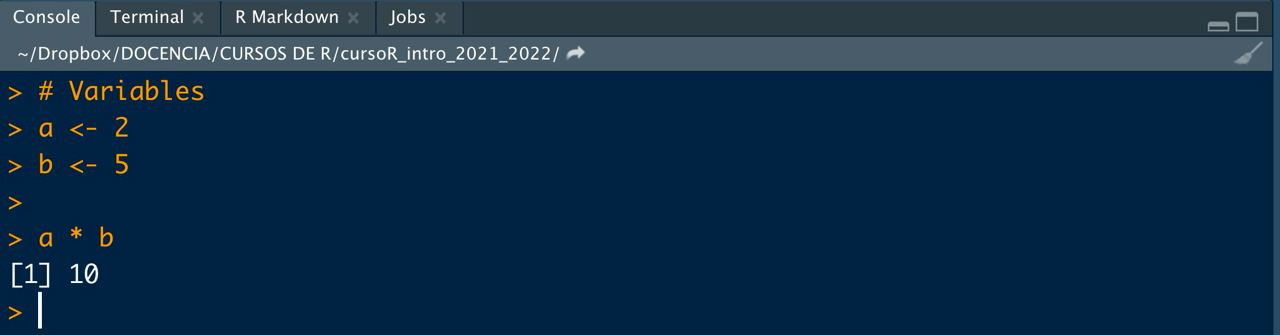
\includegraphics[width=0.8\linewidth]{./img/consola_multiplicacion} 

}

\caption{Multiplicación de a y b.}\label{fig:unnamed-chunk-4}
\end{figure}

~

📝Ejercicio 2: modifica el código inferior para definir dos variables \texttt{c} y \texttt{d}, con valores \texttt{3} y \texttt{-1}, y calcular la división \texttt{c/d} (\textbf{haz click} en la flecha para la solución propuesta).

\begin{Shaded}
\begin{Highlighting}[]
\CommentTok{# Definición de variables}
\NormalTok{c <-}\StringTok{ }
\NormalTok{d <-}

\CommentTok{# Operación (división)}
\NormalTok{c ? d}
\end{Highlighting}
\end{Shaded}

\begin{itemize}
\tightlist
\item
  Solución:
\end{itemize}

\begin{Shaded}
\begin{Highlighting}[]
\CommentTok{# Definición de variables}
\NormalTok{c <-}\StringTok{ }\DecValTok{3}
\NormalTok{d <-}\StringTok{ }\DecValTok{-1}

\CommentTok{# División}
\NormalTok{c }\OperatorTok{/}\StringTok{ }\NormalTok{d}
\end{Highlighting}
\end{Shaded}

\begin{verbatim}
## [1] -3
\end{verbatim}

~

📝Ejercicio 3: repite el ejercicio 1 pero ahora guarda el resultado de la multiplicación final en una variable \texttt{c}. Para ver el resultado guardado en \texttt{c} escribe dicha variable en consola (\textbf{haz click} en la flecha para la solución propuesta).

\begin{itemize}
\tightlist
\item
  Solución:
\end{itemize}

\begin{Shaded}
\begin{Highlighting}[]
\CommentTok{# Variables}
\NormalTok{a <-}\StringTok{ }\DecValTok{2}
\NormalTok{b <-}\StringTok{ }\DecValTok{5}

\CommentTok{# Resultado}
\NormalTok{c <-}\StringTok{ }\NormalTok{a }\OperatorTok{*}\StringTok{ }\NormalTok{b}

\CommentTok{# Muestro en consola}
\NormalTok{c}
\end{Highlighting}
\end{Shaded}

\begin{verbatim}
## [1] 10
\end{verbatim}

\begin{figure}

{\centering 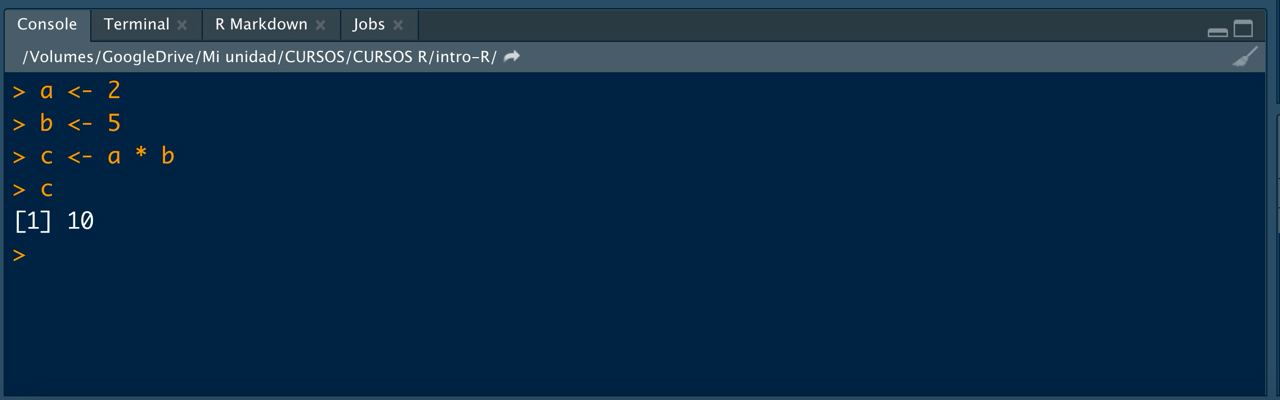
\includegraphics[width=0.8\linewidth]{./img/consola_multiplicacion_2} 

}

\caption{Multiplicación de a y b guardando el resultado.}\label{fig:unnamed-chunk-8}
\end{figure}

~

\textbf{\textcolor{#ffc107}{WARNING:}}

No hace falta gastar una línea por cada orden que quieras ejecutar. Tampoco necesitas guardar cada paso intermedio que realices. \textbf{\textcolor{#ffc107}{Cuidado con la memoria}}: cada asignación que hagas es una variable guardada que consume recursos en tu ordenador.

\hypertarget{primeros-pasos}{%
\section*{Primeros pasos}\label{primeros-pasos}}


\begin{blackbox}

Scripts usados:

\begin{itemize}
\tightlist
\item
  \href{https://github.com/dadosdelaplace/courses-intro-R/blob/main/scripts/script04.R}{\textbf{script04.R}}: primeros pasos. Ver en \url{https://github.com/dadosdelaplace/courses-intro-R/blob/main/scripts/script04.R}
\end{itemize}


\end{blackbox}

(haz click en las flechas para ver soluciones)

📝Ejercicio 1: asigna ahora los valores \texttt{1}, \texttt{-2}, \texttt{3} a tres variables \texttt{a}, \texttt{b} y \texttt{c} distintas, y calcula la raíz cuadrada de cada uno (\textbf{haz click} en la flecha para la solución propuesta).

\begin{itemize}
\tightlist
\item
  Solución:
\end{itemize}

\begin{Shaded}
\begin{Highlighting}[]
\CommentTok{# Variables}
\NormalTok{a <-}\StringTok{ }\DecValTok{1}
\NormalTok{b <-}\StringTok{ }\DecValTok{-2}
\NormalTok{c <-}\StringTok{ }\DecValTok{3}

\CommentTok{# Resultado}
\KeywordTok{sqrt}\NormalTok{(a)}
\end{Highlighting}
\end{Shaded}

\begin{verbatim}
## [1] 1
\end{verbatim}

\begin{Shaded}
\begin{Highlighting}[]
\KeywordTok{sqrt}\NormalTok{(b)}
\end{Highlighting}
\end{Shaded}

\begin{verbatim}
## [1] NaN
\end{verbatim}

\begin{Shaded}
\begin{Highlighting}[]
\KeywordTok{sqrt}\NormalTok{(c)}
\end{Highlighting}
\end{Shaded}

\begin{verbatim}
## [1] 1.732051
\end{verbatim}

~

📝Ejercicio 2: calcula en consola la suma de 3 más 4, y todo ello multiplicado por 10, y asígnalo a una variable \texttt{x} (\textbf{haz click} en la flecha para la solución propuesta). Imprime el valor por consola

\begin{itemize}
\tightlist
\item
  Solución:
\end{itemize}

\begin{Shaded}
\begin{Highlighting}[]
\CommentTok{# Asignamos}
\NormalTok{x <-}\StringTok{ }\NormalTok{(}\DecValTok{3} \OperatorTok{+}\StringTok{ }\DecValTok{4}\NormalTok{) }\OperatorTok{*}\StringTok{ }\DecValTok{10}

\CommentTok{# Imprimimos}
\NormalTok{x}
\end{Highlighting}
\end{Shaded}

\begin{verbatim}
## [1] 70
\end{verbatim}

~

📝Ejercicio 3: asigna un valor positivo a \texttt{x} y calcula su raíz cuadrada; asigna otro negativo y calcula su valor absoluto con la función \texttt{abs()} (\textbf{haz click} en la flecha para la solución propuesta).

\begin{itemize}
\tightlist
\item
  Solución:
\end{itemize}

\begin{Shaded}
\begin{Highlighting}[]
\CommentTok{# Raíz cuadrada}
\NormalTok{x <-}\StringTok{ }\DecValTok{73} \CommentTok{# por ejemplo}
\KeywordTok{sqrt}\NormalTok{(x)}
\end{Highlighting}
\end{Shaded}

\begin{verbatim}
## [1] 8.544004
\end{verbatim}

\begin{Shaded}
\begin{Highlighting}[]
\CommentTok{# Valor absoluto}
\NormalTok{y <-}\StringTok{ }\DecValTok{-19} \CommentTok{# por ejemplo}
\KeywordTok{abs}\NormalTok{(y)}
\end{Highlighting}
\end{Shaded}

\begin{verbatim}
## [1] 19
\end{verbatim}

~

\textbf{\textcolor{#20935E}{CONSEJO:}}

Las órdenes \texttt{sqrt(x)} y \texttt{abs(y)} se llaman \textbf{funciones}, y la variable que tienen entre paréntesis se llama \textbf{argumento de la función}: una variable que toma de entrada la función y con la que opera internamente.

~

📝Ejercicio 4: usando la variable \texttt{x} ya definida, completa/modifica el código inferior para guardar en una nueva variable \texttt{z} el resultado guardado en \texttt{x} menos 5 (\textbf{haz click} en la flecha para la solución propuesta).

\begin{Shaded}
\begin{Highlighting}[]
\NormalTok{z <-}\StringTok{ }\NormalTok{? }\OperatorTok{-}\StringTok{ }\NormalTok{?}
\NormalTok{z}
\end{Highlighting}
\end{Shaded}

\begin{itemize}
\tightlist
\item
  Solución:
\end{itemize}

\begin{Shaded}
\begin{Highlighting}[]
\NormalTok{z <-}\StringTok{ }\NormalTok{x }\OperatorTok{-}\StringTok{ }\DecValTok{5}
\NormalTok{z}
\end{Highlighting}
\end{Shaded}

\begin{verbatim}
## [1] 68
\end{verbatim}

~

📝Ejercicio 5: usando las variables \texttt{x} e \texttt{y} ya definidas, calcula el máximo de ambas (función \texttt{max()}), y guárdalo en una nueva variable \texttt{t}. (\textbf{haz click} en la flecha para la solución propuesta).

\begin{itemize}
\tightlist
\item
  Solución:
\end{itemize}

\begin{Shaded}
\begin{Highlighting}[]
\NormalTok{t <-}\StringTok{ }\KeywordTok{max}\NormalTok{(x, y)}
\NormalTok{t}
\end{Highlighting}
\end{Shaded}

\begin{verbatim}
## [1] 73
\end{verbatim}

~

\textbf{\textcolor{#ffc107}{WARNING:}}

No hace falta gastar una línea por cada orden que quieras ejecutar. Tampoco necesitas guardar cada paso intermedio que realices. \textbf{\textcolor{#ffc107}{Cuidado con la memoria}}: cada asignación que hagas es una variable guardada que consume recursos en tu ordenador.

\hypertarget{variables-numuxe9ricas-y-de-texto}{%
\section{Variables numéricas y de texto}\label{variables-numuxe9ricas-y-de-texto}}

\begin{blackbox}

Scripts usados:

\begin{itemize}
\tightlist
\item
  \href{https://github.com/dadosdelaplace/courses-intro-R/blob/main/scripts/script05.R}{\textbf{script05.R}}: variables numéricas y caracteres. Ver en \url{https://github.com/dadosdelaplace/courses-intro-R/blob/main/scripts/script05.R}
\end{itemize}


\end{blackbox}

(haz click en las flechas para ver soluciones)

📝Ejercicio 1: define una variable \texttt{edad} que guarde tu edad y otra \texttt{nombre} con tu nombre.

\begin{itemize}
\tightlist
\item
  Solución:
\end{itemize}

\begin{Shaded}
\begin{Highlighting}[]
\NormalTok{edad <-}\StringTok{ }\DecValTok{32} \CommentTok{# tipo numeric}
\NormalTok{nombre <-}\StringTok{ "Javier"} \CommentTok{# tipo caracter}

\NormalTok{edad}
\end{Highlighting}
\end{Shaded}

\begin{verbatim}
## [1] 32
\end{verbatim}

\begin{Shaded}
\begin{Highlighting}[]
\NormalTok{nombre}
\end{Highlighting}
\end{Shaded}

\begin{verbatim}
## [1] "Javier"
\end{verbatim}

~

📝Ejercicio 2: define otra variable con tus apellidos y junta las variables \texttt{nombre} y \texttt{apellidos} en una sola cadena de texto que guardes en \texttt{nombre\_completo}.

\begin{itemize}
\tightlist
\item
  Solución:
\end{itemize}

\begin{Shaded}
\begin{Highlighting}[]
\KeywordTok{library}\NormalTok{(glue)}
\CommentTok{# Apellidos}
\NormalTok{apellidos <-}\StringTok{ "Álvarez Liébana"}

\CommentTok{# Pegamos}
\NormalTok{nombre_completo <-}\StringTok{ }\KeywordTok{glue}\NormalTok{(}\StringTok{"\{nombre\} \{apellidos\}"}\NormalTok{)}
\NormalTok{nombre_completo}
\end{Highlighting}
\end{Shaded}

\begin{verbatim}
## Javier Álvarez Liébana
\end{verbatim}

\begin{Shaded}
\begin{Highlighting}[]
\CommentTok{# Otra forma}
\NormalTok{nombre_completo <-}\StringTok{ }\KeywordTok{paste}\NormalTok{(nombre, apellidos)}
\NormalTok{nombre_completo}
\end{Highlighting}
\end{Shaded}

\begin{verbatim}
## [1] "Javier Álvarez Liébana"
\end{verbatim}

~

📝Ejercicio 3: define dos variables numéricas y realiza la suma de ambas. Obtén con \texttt{class()} la clase de dicha variable suma

\begin{itemize}
\tightlist
\item
  Solución:
\end{itemize}

\begin{Shaded}
\begin{Highlighting}[]
\CommentTok{# Definimos dos variables numéricas}
\NormalTok{a <-}\StringTok{ }\DecValTok{1}
\NormalTok{b <-}\StringTok{ }\DecValTok{-2}

\NormalTok{a }\OperatorTok{+}\StringTok{ }\NormalTok{b}
\end{Highlighting}
\end{Shaded}

\begin{verbatim}
## [1] -1
\end{verbatim}

\begin{Shaded}
\begin{Highlighting}[]
\KeywordTok{class}\NormalTok{(a }\OperatorTok{+}\StringTok{ }\NormalTok{b)}
\end{Highlighting}
\end{Shaded}

\begin{verbatim}
## [1] "numeric"
\end{verbatim}

~

📝Ejercicio 4: construye una frase que diga «Hola, me llamo \ldots{} y tengo \ldots{} años».

\begin{itemize}
\tightlist
\item
  Solución:
\end{itemize}

\begin{Shaded}
\begin{Highlighting}[]
\NormalTok{edad <-}\StringTok{ }\DecValTok{32}
\KeywordTok{glue}\NormalTok{(}\StringTok{"Hola, me llamo \{nombre_completo\} y tengo \{edad\} años"}\NormalTok{)}
\end{Highlighting}
\end{Shaded}

\begin{verbatim}
## Hola, me llamo Javier Álvarez Liébana y tengo 32 años
\end{verbatim}

~

📝Ejercicio 5: define una cadena de texto con \texttt{"mi\ código\ postal\ es\ 28045"}. Calcula la longitud de la cadena y extrae la subcadena del lugar 3 al 17 con \texttt{str\_sub()} del paquete \texttt{\{stringr\}} (guarda dicha subcadena en una variable \texttt{y})

\begin{itemize}
\tightlist
\item
  Solución:
\end{itemize}

\begin{Shaded}
\begin{Highlighting}[]
\KeywordTok{library}\NormalTok{(stringr)}
\NormalTok{x <-}\StringTok{ "mi código postal es 28045"}
\NormalTok{y <-}\StringTok{ }\KeywordTok{str_sub}\NormalTok{(x, }\DecValTok{3}\NormalTok{, }\DecValTok{17}\NormalTok{)}
\NormalTok{y}
\end{Highlighting}
\end{Shaded}

\begin{verbatim}
## [1] " código postal "
\end{verbatim}

~

📝Ejercicio 6: con la subcadena \texttt{y} del ejercicio anterior, elimina los espacios solo de la izquierda y convierte a mayúsculas

\begin{itemize}
\tightlist
\item
  Solución:
\end{itemize}

\begin{Shaded}
\begin{Highlighting}[]
\CommentTok{# Todo en una línea}
\KeywordTok{str_to_upper}\NormalTok{(}\KeywordTok{str_trim}\NormalTok{(y, }\DataTypeTok{side =} \StringTok{"left"}\NormalTok{))}
\end{Highlighting}
\end{Shaded}

\begin{verbatim}
## [1] "CÓDIGO POSTAL "
\end{verbatim}

\begin{Shaded}
\begin{Highlighting}[]
\CommentTok{# Paso a paso}
\NormalTok{z <-}\StringTok{ }\KeywordTok{str_trim}\NormalTok{(y, }\DataTypeTok{side =} \StringTok{"left"}\NormalTok{)}
\KeywordTok{str_to_upper}\NormalTok{(z)}
\end{Highlighting}
\end{Shaded}

\begin{verbatim}
## [1] "CÓDIGO POSTAL "
\end{verbatim}

~

📝Ejercicio 7: con la cadena \texttt{x} original, sustituye la subcadena ``código postal'' por ``cp''.

\begin{itemize}
\tightlist
\item
  Solución:
\end{itemize}

\begin{Shaded}
\begin{Highlighting}[]
\KeywordTok{str_sub}\NormalTok{(x, }\DecValTok{4}\NormalTok{, }\DecValTok{16}\NormalTok{) <-}\StringTok{ "cp"}
\end{Highlighting}
\end{Shaded}

~

\hypertarget{vectores}{%
\section{Vectores}\label{vectores}}

\begin{blackbox}

Scripts usados:

\begin{itemize}
\tightlist
\item
  \href{https://github.com/dadosdelaplace/courses-intro-R/blob/main/scripts/script06.R}{\textbf{script06.R}}: vectores. Ver en \url{https://github.com/dadosdelaplace/courses-intro-R/blob/main/scripts/script06.R}
\end{itemize}


\end{blackbox}

(haz click en las flechas para ver soluciones)

📝Ejercicio 1: modifica el código inferior para crear un vector de nombre \texttt{vector\_num} que contenga los números 1, 5 y -7.

\begin{Shaded}
\begin{Highlighting}[]
\CommentTok{# Vector de números}
\NormalTok{vector_num <-}\StringTok{ }\KeywordTok{c}\NormalTok{(}\DecValTok{1}\NormalTok{)}
\NormalTok{vector_num}
\end{Highlighting}
\end{Shaded}

\begin{itemize}
\tightlist
\item
  Solución:
\end{itemize}

\begin{Shaded}
\begin{Highlighting}[]
\CommentTok{# Vector de números}
\NormalTok{vector_num <-}\StringTok{ }\KeywordTok{c}\NormalTok{(}\DecValTok{1}\NormalTok{, }\DecValTok{5}\NormalTok{, }\DecValTok{-7}\NormalTok{)}
\NormalTok{vector_num}
\end{Highlighting}
\end{Shaded}

\begin{verbatim}
## [1]  1  5 -7
\end{verbatim}

~

📝Ejercicio 2: define un vector que contenga los números 1, 10, -1 y 2, y guárdalo en una variable llamada \texttt{vector\_num}.

\begin{itemize}
\tightlist
\item
  Solución:
\end{itemize}

\begin{Shaded}
\begin{Highlighting}[]
\CommentTok{# Vector de números}
\NormalTok{vector_num <-}\StringTok{ }\KeywordTok{c}\NormalTok{(}\DecValTok{1}\NormalTok{, }\DecValTok{10}\NormalTok{, }\DecValTok{-1}\NormalTok{, }\DecValTok{2}\NormalTok{)}
\NormalTok{vector_num}
\end{Highlighting}
\end{Shaded}

\begin{verbatim}
## [1]  1 10 -1  2
\end{verbatim}

~

📝Ejercicio 3: obtén la longitud del vector anterior \texttt{vector\_num}.

\begin{itemize}
\tightlist
\item
  Solución:
\end{itemize}

\begin{Shaded}
\begin{Highlighting}[]
\CommentTok{# Longitud del vector}
\KeywordTok{length}\NormalTok{(vector_num)}
\end{Highlighting}
\end{Shaded}

\begin{verbatim}
## [1] 4
\end{verbatim}

~

📝Ejercicio 4: crea un vector con las palabras ``Hola'', ``me'', ``llamo'' (y tu nombre y apellidos), y pega luego sus elementos de forma que la frase esté correctamente escrita en castellano. Tras hacerlo, añade ``y tengo 30 años''.

\begin{itemize}
\tightlist
\item
  Solución:
\end{itemize}

\begin{Shaded}
\begin{Highlighting}[]
\CommentTok{# Definiendo el vector}
\NormalTok{vector_char <-}\StringTok{ }\KeywordTok{c}\NormalTok{(}\StringTok{"Hola"}\NormalTok{, }\StringTok{"me"}\NormalTok{, }\StringTok{"llamo"}\NormalTok{, }\StringTok{"Javier"}\NormalTok{,}
                 \StringTok{"Álvarez"}\NormalTok{, }\StringTok{"Liébana"}\NormalTok{)}

\CommentTok{# Pegamos}
\NormalTok{frase <-}\StringTok{ }\KeywordTok{paste}\NormalTok{(vector_char, }\DataTypeTok{collapse =} \StringTok{" "}\NormalTok{)}
\NormalTok{frase}
\end{Highlighting}
\end{Shaded}

\begin{verbatim}
## [1] "Hola me llamo Javier Álvarez Liébana"
\end{verbatim}

\begin{Shaded}
\begin{Highlighting}[]
\CommentTok{# Añadimos frase}
\KeywordTok{glue}\NormalTok{(}\StringTok{"\{frase\} y tengo 30 años."}\NormalTok{)}
\end{Highlighting}
\end{Shaded}

\begin{verbatim}
## Hola me llamo Javier Álvarez Liébana y tengo 30 años.
\end{verbatim}

\begin{Shaded}
\begin{Highlighting}[]
\CommentTok{# Otra forma}
\KeywordTok{paste0}\NormalTok{(frase, }\StringTok{" y tengo 30 años."}\NormalTok{)}
\end{Highlighting}
\end{Shaded}

\begin{verbatim}
## [1] "Hola me llamo Javier Álvarez Liébana y tengo 30 años."
\end{verbatim}

\begin{Shaded}
\begin{Highlighting}[]
\CommentTok{# Otra forma}
\KeywordTok{paste}\NormalTok{(frase, }\StringTok{"y tengo 30 años."}\NormalTok{)}
\end{Highlighting}
\end{Shaded}

\begin{verbatim}
## [1] "Hola me llamo Javier Álvarez Liébana y tengo 30 años."
\end{verbatim}

~

📝Ejercicio 5: el código inferior crea una secuencia de números, que empieza en \texttt{-1}, que acaba en \texttt{32}, y que va saltando de 2 en 2. Modíficalo para que haga el salto de 3 en 3 y guárdalo en una variable llamada \texttt{secuencia}

\begin{Shaded}
\begin{Highlighting}[]
\KeywordTok{seq}\NormalTok{(}\OperatorTok{-}\DecValTok{1}\NormalTok{, }\DecValTok{32}\NormalTok{, }\DataTypeTok{by =} \DecValTok{2}\NormalTok{)}
\end{Highlighting}
\end{Shaded}

\begin{itemize}
\tightlist
\item
  Solución:
\end{itemize}

\begin{Shaded}
\begin{Highlighting}[]
\NormalTok{secuencia <-}\StringTok{ }\KeywordTok{seq}\NormalTok{(}\OperatorTok{-}\DecValTok{1}\NormalTok{, }\DecValTok{32}\NormalTok{, }\DataTypeTok{by =} \DecValTok{3}\NormalTok{)}
\NormalTok{secuencia}
\end{Highlighting}
\end{Shaded}

\begin{verbatim}
##  [1] -1  2  5  8 11 14 17 20 23 26 29 32
\end{verbatim}

\begin{Shaded}
\begin{Highlighting}[]
\KeywordTok{length}\NormalTok{(secuencia) }\CommentTok{# longitud de la secuencia}
\end{Highlighting}
\end{Shaded}

\begin{verbatim}
## [1] 12
\end{verbatim}

~

📝Ejercicio 6: crea una secuencia de números, que empiece en \texttt{-1}, que acabe en \texttt{32}, y que tenga longitud 12.

\begin{itemize}
\tightlist
\item
  Solución:
\end{itemize}

\begin{Shaded}
\begin{Highlighting}[]
\NormalTok{secuencia <-}\StringTok{ }\KeywordTok{seq}\NormalTok{(}\OperatorTok{-}\DecValTok{1}\NormalTok{, }\DecValTok{32}\NormalTok{, }\DataTypeTok{l =} \DecValTok{12}\NormalTok{)}
\NormalTok{secuencia}
\end{Highlighting}
\end{Shaded}

\begin{verbatim}
##  [1] -1  2  5  8 11 14 17 20 23 26 29 32
\end{verbatim}

\begin{Shaded}
\begin{Highlighting}[]
\KeywordTok{length}\NormalTok{(secuencia) }\CommentTok{# longitud de la secuencia}
\end{Highlighting}
\end{Shaded}

\begin{verbatim}
## [1] 12
\end{verbatim}

~

📝Ejercicio 7: crea una secuencia que empiece en 1 y recorra todos los naturales hasta el 10. Después crea otra secuencia de longitud 7 que todos los números sean \texttt{3}.

\begin{itemize}
\tightlist
\item
  Solución:
\end{itemize}

\begin{Shaded}
\begin{Highlighting}[]
\DecValTok{1}\OperatorTok{:}\DecValTok{10}
\end{Highlighting}
\end{Shaded}

\begin{verbatim}
##  [1]  1  2  3  4  5  6  7  8  9 10
\end{verbatim}

\begin{Shaded}
\begin{Highlighting}[]
\KeywordTok{rep}\NormalTok{(}\DecValTok{3}\NormalTok{, }\DecValTok{7}\NormalTok{) }\CommentTok{# secuencia repetida}
\end{Highlighting}
\end{Shaded}

\begin{verbatim}
## [1] 3 3 3 3 3 3 3
\end{verbatim}

~

📝Ejercicio 8: crea una secuencia que repita 5 veces el patrón \texttt{1,\ 2,\ 3}. Después crea otra que repita dicho patrón pero de forma intercalada, con 5 veces \texttt{1}, después 5 veces \texttt{2} y después 5 veces \texttt{3}.

\begin{itemize}
\tightlist
\item
  Solución:
\end{itemize}

\begin{Shaded}
\begin{Highlighting}[]
\KeywordTok{rep}\NormalTok{(}\KeywordTok{c}\NormalTok{(}\DecValTok{1}\NormalTok{, }\DecValTok{2}\NormalTok{, }\DecValTok{3}\NormalTok{), }\DecValTok{5}\NormalTok{) }\CommentTok{# repetimos patrón (1, 2, 3) 5 veces}
\end{Highlighting}
\end{Shaded}

\begin{verbatim}
##  [1] 1 2 3 1 2 3 1 2 3 1 2 3 1 2 3
\end{verbatim}

\begin{Shaded}
\begin{Highlighting}[]
\KeywordTok{rep}\NormalTok{(}\KeywordTok{c}\NormalTok{(}\DecValTok{1}\NormalTok{, }\DecValTok{2}\NormalTok{, }\DecValTok{3}\NormalTok{), }\DataTypeTok{each =} \DecValTok{5}\NormalTok{) }\CommentTok{# repetimos patrón alternado}
\end{Highlighting}
\end{Shaded}

\begin{verbatim}
##  [1] 1 1 1 1 1 2 2 2 2 2 3 3 3 3 3
\end{verbatim}

~

📝Ejercicio 9: crea una variable \texttt{x\ \textless{}-\ c("oso\ pardo",\ "oso\ polar",\ "ballena",\ "grillo",\ "oso\ panda",\ "perro")}. Haciendo uso de \texttt{str\_length()} calcula la longitud de cada cadena de texto. Haciendo uso de \texttt{str\_detect()} detecta los animales que son un oso.

\begin{itemize}
\tightlist
\item
  Solución:
\end{itemize}

\begin{Shaded}
\begin{Highlighting}[]
\NormalTok{x <-}\StringTok{ }\KeywordTok{c}\NormalTok{(}\StringTok{"oso pardo"}\NormalTok{, }\StringTok{"Oso polar"}\NormalTok{, }\StringTok{"ballena"}\NormalTok{, }\StringTok{"grillo"}\NormalTok{, }\StringTok{"OSO panda"}\NormalTok{, }\StringTok{"perro"}\NormalTok{)}
\KeywordTok{str_length}\NormalTok{(x) }\CommentTok{# longitud}
\end{Highlighting}
\end{Shaded}

\begin{verbatim}
## [1] 9 9 7 6 9 5
\end{verbatim}

\begin{Shaded}
\begin{Highlighting}[]
\CommentTok{# OJO! antes hay que pasar todo a mayúscula o minúscula, nos da igual que sea oso, OSO, Oso, etc}
\KeywordTok{str_detect}\NormalTok{(}\KeywordTok{str_to_lower}\NormalTok{(x), }\StringTok{"oso"}\NormalTok{) }
\end{Highlighting}
\end{Shaded}

\begin{verbatim}
## [1]  TRUE  TRUE FALSE FALSE  TRUE FALSE
\end{verbatim}

\hypertarget{operaciones-con-vectores}{%
\section{Operaciones con vectores}\label{operaciones-con-vectores}}

\begin{blackbox}

Scripts usados:

\begin{itemize}
\tightlist
\item
  \href{https://github.com/dadosdelaplace/courses-intro-R/blob/main/scripts/script07.R}{\textbf{script07.R}}: operaciones con vectores. Ver en \url{https://github.com/dadosdelaplace/courses-intro-R/blob/main/scripts/script07.R}
\end{itemize}


\end{blackbox}

(haz click en las flechas para ver soluciones)

📝Ejercicio 1: define el vector \texttt{x} como la concatenación de los números 1, 10, -1 y 2, y calcula su suma.

\begin{itemize}
\tightlist
\item
  Solución:
\end{itemize}

\begin{Shaded}
\begin{Highlighting}[]
\CommentTok{# Vector de números}
\NormalTok{x <-}\StringTok{ }\KeywordTok{c}\NormalTok{(}\DecValTok{1}\NormalTok{, }\DecValTok{10}\NormalTok{, }\DecValTok{-1}\NormalTok{, }\DecValTok{2}\NormalTok{)}

\CommentTok{# Suma}
\KeywordTok{sum}\NormalTok{(x)}
\end{Highlighting}
\end{Shaded}

\begin{verbatim}
## [1] 12
\end{verbatim}

~

📝Ejercicio 2: define otro vector \texttt{y} que contenga los números \texttt{5,\ -7,\ 8,\ -3}, y haz la suma de \texttt{x} e \texttt{y}.

\begin{itemize}
\tightlist
\item
  Solución:
\end{itemize}

\begin{Shaded}
\begin{Highlighting}[]
\CommentTok{# Vector de números}
\NormalTok{y <-}\StringTok{ }\KeywordTok{c}\NormalTok{(}\DecValTok{5}\NormalTok{, }\DecValTok{-7}\NormalTok{, }\DecValTok{8}\NormalTok{, }\DecValTok{-3}\NormalTok{)}

\CommentTok{# Suma}
\NormalTok{x }\OperatorTok{+}\StringTok{ }\NormalTok{y}
\end{Highlighting}
\end{Shaded}

\begin{verbatim}
## [1]  6  3  7 -1
\end{verbatim}

~

📝Ejercicio 3: calcula el número de elementos mayores que 0 del resultado de la suma de \texttt{x\ +\ y}.

\begin{itemize}
\tightlist
\item
  Solución:
\end{itemize}

\begin{Shaded}
\begin{Highlighting}[]
\KeywordTok{sum}\NormalTok{((x }\OperatorTok{+}\StringTok{ }\NormalTok{y) }\OperatorTok{>}\StringTok{ }\DecValTok{0}\NormalTok{)}
\end{Highlighting}
\end{Shaded}

\begin{verbatim}
## [1] 3
\end{verbatim}

\begin{Shaded}
\begin{Highlighting}[]
\CommentTok{# Otra forma}
\NormalTok{suma <-}\StringTok{ }\NormalTok{x }\OperatorTok{+}\StringTok{ }\NormalTok{y}
\KeywordTok{sum}\NormalTok{(suma }\OperatorTok{>}\StringTok{ }\DecValTok{0}\NormalTok{)}
\end{Highlighting}
\end{Shaded}

\begin{verbatim}
## [1] 3
\end{verbatim}

~

📝Ejercicio 4: calcula la versión ordenada del vector \texttt{x}.

\begin{itemize}
\tightlist
\item
  Solución:
\end{itemize}

\begin{Shaded}
\begin{Highlighting}[]
\CommentTok{# Ordenamos el vector (con sort)}
\KeywordTok{sort}\NormalTok{(x)}
\end{Highlighting}
\end{Shaded}

\begin{verbatim}
## [1] -1  1  2 10
\end{verbatim}

\begin{Shaded}
\begin{Highlighting}[]
\CommentTok{# Ordenamos el vector  (con order)}
\NormalTok{x[}\KeywordTok{order}\NormalTok{(x)]}
\end{Highlighting}
\end{Shaded}

\begin{verbatim}
## [1] -1  1  2 10
\end{verbatim}

~

📝Ejercicio 5: encuentra del vector \texttt{x} original el lugar (el índice) que ocupa su mínimo y su máximo.

\begin{itemize}
\tightlist
\item
  Solución:
\end{itemize}

\begin{Shaded}
\begin{Highlighting}[]
\NormalTok{x<-}\StringTok{ }\KeywordTok{c}\NormalTok{(}\DecValTok{1}\NormalTok{, }\DecValTok{10}\NormalTok{, }\DecValTok{-1}\NormalTok{, }\DecValTok{2}\NormalTok{)}

\CommentTok{# Encontrando el lugar que ocupa el máximo y mínimo}
\KeywordTok{which.max}\NormalTok{(x)}
\end{Highlighting}
\end{Shaded}

\begin{verbatim}
## [1] 2
\end{verbatim}

\begin{Shaded}
\begin{Highlighting}[]
\KeywordTok{which.min}\NormalTok{(x)}
\end{Highlighting}
\end{Shaded}

\begin{verbatim}
## [1] 3
\end{verbatim}

~

📝Ejercicio 6: encuentra del vector \texttt{x} los elementos mayores que 1 y menores que 7. Encuentra una forma de averiguar si todos los elementos son o no positivos.

\begin{itemize}
\tightlist
\item
  Solución:
\end{itemize}

\begin{Shaded}
\begin{Highlighting}[]
\CommentTok{# Vector lógico: mayores que 1 y menores que 7}
\NormalTok{x }\OperatorTok{>}\StringTok{ }\DecValTok{1} \OperatorTok{&}\StringTok{ }\NormalTok{x }\OperatorTok{<}\StringTok{ }\DecValTok{7}
\end{Highlighting}
\end{Shaded}

\begin{verbatim}
## [1] FALSE FALSE FALSE  TRUE
\end{verbatim}

\begin{Shaded}
\begin{Highlighting}[]
\CommentTok{# ¿Son todos positivos? Mira también any()}
\KeywordTok{all}\NormalTok{(x }\OperatorTok{>}\StringTok{ }\DecValTok{0}\NormalTok{)}
\end{Highlighting}
\end{Shaded}

\begin{verbatim}
## [1] FALSE
\end{verbatim}

~

📝Ejercicio 7: define el vector \texttt{c(-1,\ 0,\ 4,\ 5,\ -2)}, calcula la raíz cuadrada del vector y determina que lugares son ausente de tipo \texttt{NaN}.

\begin{itemize}
\tightlist
\item
  Solución:
\end{itemize}

\begin{Shaded}
\begin{Highlighting}[]
\CommentTok{# Vector}
\NormalTok{z <-}\StringTok{ }\KeywordTok{c}\NormalTok{(}\OperatorTok{-}\DecValTok{1}\NormalTok{, }\DecValTok{0}\NormalTok{, }\DecValTok{4}\NormalTok{, }\DecValTok{5}\NormalTok{, }\DecValTok{-2}\NormalTok{)}

\CommentTok{# ¿Cuáles son ausentes tras aplicar la raíz cuadrada?}
\KeywordTok{is.nan}\NormalTok{(}\KeywordTok{sqrt}\NormalTok{(z))}
\end{Highlighting}
\end{Shaded}

\begin{verbatim}
## [1]  TRUE FALSE FALSE FALSE  TRUE
\end{verbatim}

~

📝Ejercicio 8: define el vector de los primeros números impares (hasta el 21) y extrae los elementos que ocupan los lugares 1, 4, 5, 8. Elimina del vector el segundo elemento

\begin{itemize}
\tightlist
\item
  Solución:
\end{itemize}

\begin{Shaded}
\begin{Highlighting}[]
\CommentTok{# Vector de impares (de 1 a 21 saltando de dos en dos)}
\NormalTok{x <-}\StringTok{ }\KeywordTok{seq}\NormalTok{(}\DecValTok{1}\NormalTok{, }\DecValTok{21}\NormalTok{, }\DataTypeTok{by =} \DecValTok{2}\NormalTok{)}

\CommentTok{# Seleccionamos elementos}
\NormalTok{x[}\KeywordTok{c}\NormalTok{(}\DecValTok{1}\NormalTok{, }\DecValTok{4}\NormalTok{, }\DecValTok{5}\NormalTok{, }\DecValTok{8}\NormalTok{)]}
\end{Highlighting}
\end{Shaded}

\begin{verbatim}
## [1]  1  7  9 15
\end{verbatim}

\begin{Shaded}
\begin{Highlighting}[]
\CommentTok{# Eliminamos elementos}
\NormalTok{y <-}\StringTok{ }\NormalTok{x[}\OperatorTok{-}\DecValTok{2}\NormalTok{]}
\NormalTok{y}
\end{Highlighting}
\end{Shaded}

\begin{verbatim}
##  [1]  1  5  7  9 11 13 15 17 19 21
\end{verbatim}

~

📝Ejercicio 9: define una cadena de caracteres \texttt{texto\ \textless{}-\ c("oso\ polar",\ "oso\ pardo",\ "salamandra",\ "buho",\ "lechuza",\ "oso\ malayo")}. Usa \texttt{str\_count()} para contabilizar el número de osos. Usa \texttt{str\_starts()} para saber que elemento del vector es un oso o no. Obten la longitud de cada cadena. Sustituye en todas las cadenas la \texttt{o} por \texttt{*}

\begin{itemize}
\tightlist
\item
  Solución:
\end{itemize}

\begin{Shaded}
\begin{Highlighting}[]
\NormalTok{texto <-}\StringTok{ }\KeywordTok{c}\NormalTok{(}\StringTok{"oso polar"}\NormalTok{, }\StringTok{"oso pardo"}\NormalTok{, }\StringTok{"salamandra"}\NormalTok{, }\StringTok{"buho"}\NormalTok{, }\StringTok{"lechuza"}\NormalTok{, }\StringTok{"oso malayo"}\NormalTok{)}

\CommentTok{# Cuenta el número de cadenas que contienen la palabra "oso"}
\KeywordTok{str_count}\NormalTok{(texto, }\StringTok{"oso"}\NormalTok{)}
\end{Highlighting}
\end{Shaded}

\begin{verbatim}
## [1] 1 1 0 0 0 1
\end{verbatim}

\begin{Shaded}
\begin{Highlighting}[]
\CommentTok{# Nos devuelve TRUE en las cadenas que empiecen por "oso"}
\KeywordTok{str_starts}\NormalTok{(texto, }\StringTok{"oso"}\NormalTok{)}
\end{Highlighting}
\end{Shaded}

\begin{verbatim}
## [1]  TRUE  TRUE FALSE FALSE FALSE  TRUE
\end{verbatim}

\begin{Shaded}
\begin{Highlighting}[]
\KeywordTok{str_ends}\NormalTok{(texto, }\StringTok{"oso"}\NormalTok{) }\CommentTok{# devuelve todo FALSE}
\end{Highlighting}
\end{Shaded}

\begin{verbatim}
## [1] FALSE FALSE FALSE FALSE FALSE FALSE
\end{verbatim}

\begin{Shaded}
\begin{Highlighting}[]
\CommentTok{# Longitud de cada cadena}
\KeywordTok{str_length}\NormalTok{(texto)}
\end{Highlighting}
\end{Shaded}

\begin{verbatim}
## [1]  9  9 10  4  7 10
\end{verbatim}

\begin{Shaded}
\begin{Highlighting}[]
\CommentTok{# Sustituimos en todas las oes por *}
\KeywordTok{str_replace_all}\NormalTok{(texto, }\StringTok{"o"}\NormalTok{, }\StringTok{"*"}\NormalTok{)}
\end{Highlighting}
\end{Shaded}

\begin{verbatim}
## [1] "*s* p*lar"  "*s* pard*"  "salamandra" "buh*"       "lechuza"   
## [6] "*s* malay*"
\end{verbatim}

\hypertarget{fechas}{%
\section{Fechas}\label{fechas}}

\begin{blackbox}

Scripts usados:

\begin{itemize}
\tightlist
\item
  \href{https://github.com/dadosdelaplace/courses-intro-R/blob/main/scripts/script08.R}{\textbf{script08.R}}: operaciones con vectores. Ver en \url{https://github.com/dadosdelaplace/courses-intro-R/blob/main/scripts/script08.R}
\end{itemize}


\end{blackbox}

(haz click en las flechas para ver soluciones)

📝Ejercicio 1: obten la fecha de hoy, define la fecha de tu cumpleaños, y calcula la diferencia de días.

\begin{itemize}
\tightlist
\item
  Solución:
\end{itemize}

\begin{Shaded}
\begin{Highlighting}[]
\KeywordTok{library}\NormalTok{(lubridate)}
\CommentTok{# Hoy}
\NormalTok{hoy <-}\StringTok{ }\KeywordTok{today}\NormalTok{()}

\CommentTok{# Cumple (diferentes formatos de entrada)}
\NormalTok{cumple <-}\StringTok{ }\KeywordTok{as_date}\NormalTok{(}\StringTok{"1989-09-10"}\NormalTok{) }\CommentTok{# por defecto}
\NormalTok{cumple <-}\StringTok{ }\KeywordTok{as_date}\NormalTok{(}\StringTok{"10-09-1989"}\NormalTok{, }\DataTypeTok{format =} \StringTok{"%d-%m-%Y"}\NormalTok{)}

\CommentTok{# Diferencia}
\NormalTok{hoy }\OperatorTok{-}\StringTok{ }\NormalTok{cumple}
\end{Highlighting}
\end{Shaded}

\begin{verbatim}
## Time difference of 12000 days
\end{verbatim}

~

📝Ejercicio 2: define la fecha de tu cumpleaños y determina si fue año bisiesto. Súmale 1-2-3-4-5 semanas.

\begin{itemize}
\tightlist
\item
  Solución:
\end{itemize}

\begin{Shaded}
\begin{Highlighting}[]
\NormalTok{cumple <-}\StringTok{ }\KeywordTok{as_date}\NormalTok{(}\StringTok{"1989-09-10"}\NormalTok{) }\CommentTok{# por defecto}

\CommentTok{# Bisiesto}
\KeywordTok{leap_year}\NormalTok{(cumple)}
\end{Highlighting}
\end{Shaded}

\begin{verbatim}
## [1] FALSE
\end{verbatim}

\begin{Shaded}
\begin{Highlighting}[]
\CommentTok{# Sumamos semanaes}
\NormalTok{cumple }\OperatorTok{+}\StringTok{ }\KeywordTok{weeks}\NormalTok{(}\DecValTok{1}\OperatorTok{:}\DecValTok{5}\NormalTok{)}
\end{Highlighting}
\end{Shaded}

\begin{verbatim}
## [1] "1989-09-17" "1989-09-24" "1989-10-01" "1989-10-08" "1989-10-15"
\end{verbatim}

~

📝Ejercicio 3: extrae el mes, año y día de la semana de tu cumpleaños

\begin{itemize}
\tightlist
\item
  Solución:
\end{itemize}

\begin{Shaded}
\begin{Highlighting}[]
\CommentTok{# Mes}
\KeywordTok{month}\NormalTok{(cumple)}
\end{Highlighting}
\end{Shaded}

\begin{verbatim}
## [1] 9
\end{verbatim}

\begin{Shaded}
\begin{Highlighting}[]
\CommentTok{# Año }
\KeywordTok{year}\NormalTok{(cumple)}
\end{Highlighting}
\end{Shaded}

\begin{verbatim}
## [1] 1989
\end{verbatim}

\begin{Shaded}
\begin{Highlighting}[]
\CommentTok{# wday}
\KeywordTok{wday}\NormalTok{(cumple, }\DataTypeTok{week_start =} \DecValTok{1}\NormalTok{)}
\end{Highlighting}
\end{Shaded}

\begin{verbatim}
## [1] 7
\end{verbatim}

\begin{Shaded}
\begin{Highlighting}[]
\KeywordTok{wday}\NormalTok{(cumple, }\DataTypeTok{week_start =} \DecValTok{1}\NormalTok{, }\DataTypeTok{label =} \OtherTok{TRUE}\NormalTok{)}
\end{Highlighting}
\end{Shaded}

\begin{verbatim}
## [1] Sun
## Levels: Mon < Tue < Wed < Thu < Fri < Sat < Sun
\end{verbatim}

~

📝Ejercicio 4: calcula los días que han pasado desde la fecha de tu nacimiento

\begin{itemize}
\tightlist
\item
  Solución:
\end{itemize}

\begin{Shaded}
\begin{Highlighting}[]
\KeywordTok{seconds}\NormalTok{(}\KeywordTok{today}\NormalTok{() }\OperatorTok{-}\StringTok{ }\NormalTok{cumple)}
\end{Highlighting}
\end{Shaded}

\begin{verbatim}
## [1] "12000S"
\end{verbatim}

~

\hypertarget{datos-estructurados}{%
\section{Datos estructurados}\label{datos-estructurados}}

\begin{blackbox}

Scripts usados:

\begin{itemize}
\tightlist
\item
  \href{https://github.com/dadosdelaplace/courses-intro-R/blob/main/scripts/script09.R}{\textbf{script09.R}}: datos estructurados. Ver en \url{https://github.com/dadosdelaplace/courses-intro-R/blob/main/scripts/script09.R}
\end{itemize}


\end{blackbox}

(haz click en las flechas para ver soluciones)

Ejercicio 1: modifica el código para definir una matriz \texttt{x} de ceros de 3 filas y 7 columnas.

\begin{Shaded}
\begin{Highlighting}[]
\CommentTok{# Matriz}
\NormalTok{x <-}\StringTok{ }\KeywordTok{matrix}\NormalTok{(}\DecValTok{0}\NormalTok{, }\DataTypeTok{nrow =} \DecValTok{2}\NormalTok{, }\DataTypeTok{ncol =} \DecValTok{3}\NormalTok{)}
\NormalTok{x}
\end{Highlighting}
\end{Shaded}

\begin{itemize}
\tightlist
\item
  Solución:
\end{itemize}

\begin{Shaded}
\begin{Highlighting}[]
\CommentTok{# Matriz}
\NormalTok{x <-}\StringTok{ }\KeywordTok{matrix}\NormalTok{(}\DecValTok{0}\NormalTok{, }\DataTypeTok{nrow =} \DecValTok{3}\NormalTok{, }\DataTypeTok{ncol =} \DecValTok{7}\NormalTok{)}
\NormalTok{x}
\end{Highlighting}
\end{Shaded}

\begin{verbatim}
##      [,1] [,2] [,3] [,4] [,5] [,6] [,7]
## [1,]    0    0    0    0    0    0    0
## [2,]    0    0    0    0    0    0    0
## [3,]    0    0    0    0    0    0    0
\end{verbatim}

~

Ejercicio 2: a la matriz anterior, suma un 1 a cada número de la matriz y divide el resultado entre 5.

\begin{itemize}
\tightlist
\item
  Solución:
\end{itemize}

\begin{Shaded}
\begin{Highlighting}[]
\NormalTok{(x }\OperatorTok{+}\StringTok{ }\DecValTok{1}\NormalTok{) }\OperatorTok{/}\StringTok{ }\DecValTok{5}
\end{Highlighting}
\end{Shaded}

\begin{verbatim}
##      [,1] [,2] [,3] [,4] [,5] [,6] [,7]
## [1,]  0.2  0.2  0.2  0.2  0.2  0.2  0.2
## [2,]  0.2  0.2  0.2  0.2  0.2  0.2  0.2
## [3,]  0.2  0.2  0.2  0.2  0.2  0.2  0.2
\end{verbatim}

~

Ejercicio 3: tras definir la matriz \texttt{x} calcula su transpuesta y obtén sus dimensiones

\begin{itemize}
\tightlist
\item
  Solución:
\end{itemize}

\begin{Shaded}
\begin{Highlighting}[]
\CommentTok{# Transpuesta}
\KeywordTok{t}\NormalTok{(x)}
\end{Highlighting}
\end{Shaded}

\begin{verbatim}
##      [,1] [,2] [,3]
## [1,]    0    0    0
## [2,]    0    0    0
## [3,]    0    0    0
## [4,]    0    0    0
## [5,]    0    0    0
## [6,]    0    0    0
## [7,]    0    0    0
\end{verbatim}

\begin{Shaded}
\begin{Highlighting}[]
\CommentTok{# Dimensiones transpuesta: pasa de ser 3x7 a 7x3}
\KeywordTok{dim}\NormalTok{(}\KeywordTok{t}\NormalTok{(x))}
\end{Highlighting}
\end{Shaded}

\begin{verbatim}
## [1] 7 3
\end{verbatim}

\begin{Shaded}
\begin{Highlighting}[]
\KeywordTok{ncol}\NormalTok{(}\KeywordTok{t}\NormalTok{(x)) }\CommentTok{# número de columnas de la transpuesta}
\end{Highlighting}
\end{Shaded}

\begin{verbatim}
## [1] 3
\end{verbatim}

\begin{Shaded}
\begin{Highlighting}[]
\KeywordTok{nrow}\NormalTok{(}\KeywordTok{t}\NormalTok{(x)) }\CommentTok{# número de filas de la transpuesta}
\end{Highlighting}
\end{Shaded}

\begin{verbatim}
## [1] 7
\end{verbatim}

~

Ejercicio 4: el siguiente código define una matriz de dimensiones \texttt{4\ x\ 3} y calcula la suma por columnas. Modifica el código para que realice la suma por filas.

\begin{Shaded}
\begin{Highlighting}[]
\CommentTok{# Matriz}
\NormalTok{matriz <-}\StringTok{ }\KeywordTok{matrix}\NormalTok{(}\DecValTok{1}\OperatorTok{:}\DecValTok{12}\NormalTok{, }\DataTypeTok{nrow =} \DecValTok{4}\NormalTok{)}

\CommentTok{# Suma por columnas}
\KeywordTok{apply}\NormalTok{(matriz, }\DataTypeTok{MARGIN =} \DecValTok{2}\NormalTok{, }\DataTypeTok{FUN =} \StringTok{"sum"}\NormalTok{)}
\end{Highlighting}
\end{Shaded}

\begin{verbatim}
## [1] 10 26 42
\end{verbatim}

\begin{itemize}
\tightlist
\item
  Solución:
\end{itemize}

\begin{Shaded}
\begin{Highlighting}[]
\CommentTok{# Matriz}
\NormalTok{matriz <-}\StringTok{ }\KeywordTok{matrix}\NormalTok{(}\DecValTok{1}\OperatorTok{:}\DecValTok{12}\NormalTok{, }\DataTypeTok{nrow =} \DecValTok{4}\NormalTok{)}

\CommentTok{# Suma por filas}
\KeywordTok{apply}\NormalTok{(matriz, }\DataTypeTok{MARGIN =} \DecValTok{1}\NormalTok{, }\DataTypeTok{FUN =} \StringTok{"sum"}\NormalTok{)}
\end{Highlighting}
\end{Shaded}

\begin{verbatim}
## [1] 15 18 21 24
\end{verbatim}

~

Ejercicio 5: con la matriz anterior definida como \texttt{matrix(1:12,\ nrow\ =\ 4)}, calcula la media de todos los elementos, la media de cada fila y la media de cada columna.

\begin{itemize}
\tightlist
\item
  Solución:
\end{itemize}

\begin{Shaded}
\begin{Highlighting}[]
\CommentTok{# Matriz}
\NormalTok{matriz <-}\StringTok{ }\KeywordTok{matrix}\NormalTok{(}\DecValTok{1}\OperatorTok{:}\DecValTok{12}\NormalTok{, }\DataTypeTok{nrow =} \DecValTok{4}\NormalTok{)}

\CommentTok{#  media de todos}
\KeywordTok{mean}\NormalTok{(matriz)}
\end{Highlighting}
\end{Shaded}

\begin{verbatim}
## [1] 6.5
\end{verbatim}

\begin{Shaded}
\begin{Highlighting}[]
\CommentTok{# Media por filas (MARGIN = 1 ya que es una operación por filas)}
\KeywordTok{apply}\NormalTok{(matriz, }\DataTypeTok{MARGIN =} \DecValTok{1}\NormalTok{, }\DataTypeTok{FUN =} \StringTok{"mean"}\NormalTok{)}
\end{Highlighting}
\end{Shaded}

\begin{verbatim}
## [1] 5 6 7 8
\end{verbatim}

\begin{Shaded}
\begin{Highlighting}[]
\CommentTok{# Media por filas (MARGIN = 2 ya que es una operación por filas)}
\KeywordTok{apply}\NormalTok{(matriz, }\DataTypeTok{MARGIN =} \DecValTok{2}\NormalTok{, }\DataTypeTok{FUN =} \StringTok{"mean"}\NormalTok{)}
\end{Highlighting}
\end{Shaded}

\begin{verbatim}
## [1]  2.5  6.5 10.5
\end{verbatim}

~

Ejercicio 6: el \texttt{data.frame} llamado \texttt{airquality}, del paquete \texttt{\{datasets\}}, contiene variables de la calidad del aire de la ciudad de Nueva York desde mayo hasta septiembre de 1973. Obtén el nombre de las variables.

\begin{itemize}
\tightlist
\item
  Solución:
\end{itemize}

\begin{Shaded}
\begin{Highlighting}[]
\KeywordTok{library}\NormalTok{(datasets)}
\KeywordTok{names}\NormalTok{(airquality)}
\end{Highlighting}
\end{Shaded}

\begin{verbatim}
## [1] "Ozone"   "Solar.R" "Wind"    "Temp"    "Month"   "Day"
\end{verbatim}

~

Ejercicio 7: obtén las dimensiones del conjunto de datos. ¿Cuántas variables hay? ¿Cuántos días se han medido?

\begin{itemize}
\tightlist
\item
  Solución:
\end{itemize}

\begin{Shaded}
\begin{Highlighting}[]
\CommentTok{# Dimensiones}
\KeywordTok{dim}\NormalTok{(airquality)}
\end{Highlighting}
\end{Shaded}

\begin{verbatim}
## [1] 153   6
\end{verbatim}

\begin{Shaded}
\begin{Highlighting}[]
\KeywordTok{nrow}\NormalTok{(airquality)}
\end{Highlighting}
\end{Shaded}

\begin{verbatim}
## [1] 153
\end{verbatim}

\begin{Shaded}
\begin{Highlighting}[]
\KeywordTok{ncol}\NormalTok{(airquality)}
\end{Highlighting}
\end{Shaded}

\begin{verbatim}
## [1] 6
\end{verbatim}

~

Ejercicio 8: modifica el código inferior para que nos filtre solo los datos del mes de julio.

\begin{Shaded}
\begin{Highlighting}[]
\CommentTok{# Filtramos filas}
\NormalTok{filtro_fila <-}\StringTok{ }\KeywordTok{subset}\NormalTok{(., }\DataTypeTok{subset =}\NormalTok{ Month }\OperatorTok{<}\StringTok{ }\DecValTok{6}\NormalTok{)}
\NormalTok{filtro_fila}
\end{Highlighting}
\end{Shaded}

\begin{itemize}
\tightlist
\item
  Solución:
\end{itemize}

\begin{Shaded}
\begin{Highlighting}[]
\CommentTok{# Filtramos filas}
\NormalTok{filtro_fila <-}\StringTok{ }\KeywordTok{subset}\NormalTok{(airquality, }\DataTypeTok{subset =}\NormalTok{ Month }\OperatorTok{==}\StringTok{ }\DecValTok{7}\NormalTok{)}
\NormalTok{filtro_fila}
\end{Highlighting}
\end{Shaded}

\begin{verbatim}
##    Ozone Solar.R Wind Temp Month Day
## 62   135     269  4.1   84     7   1
## 63    49     248  9.2   85     7   2
## 64    32     236  9.2   81     7   3
## 65    NA     101 10.9   84     7   4
## 66    64     175  4.6   83     7   5
## 67    40     314 10.9   83     7   6
## 68    77     276  5.1   88     7   7
## 69    97     267  6.3   92     7   8
## 70    97     272  5.7   92     7   9
## 71    85     175  7.4   89     7  10
## 72    NA     139  8.6   82     7  11
## 73    10     264 14.3   73     7  12
## 74    27     175 14.9   81     7  13
## 75    NA     291 14.9   91     7  14
## 76     7      48 14.3   80     7  15
## 77    48     260  6.9   81     7  16
## 78    35     274 10.3   82     7  17
## 79    61     285  6.3   84     7  18
## 80    79     187  5.1   87     7  19
## 81    63     220 11.5   85     7  20
## 82    16       7  6.9   74     7  21
## 83    NA     258  9.7   81     7  22
## 84    NA     295 11.5   82     7  23
## 85    80     294  8.6   86     7  24
## 86   108     223  8.0   85     7  25
## 87    20      81  8.6   82     7  26
## 88    52      82 12.0   86     7  27
## 89    82     213  7.4   88     7  28
## 90    50     275  7.4   86     7  29
## 91    64     253  7.4   83     7  30
## 92    59     254  9.2   81     7  31
\end{verbatim}

~

Ejercicio 9: del conjunto \texttt{airquality} selecciona aquellos datos que no sean ni de julio ni de agosto.

\begin{itemize}
\tightlist
\item
  Solución:
\end{itemize}

\begin{Shaded}
\begin{Highlighting}[]
\CommentTok{# Filtramos filas}
\NormalTok{filtro_fila <-}
\StringTok{  }\KeywordTok{subset}\NormalTok{(airquality, }\DataTypeTok{subset =} \OperatorTok{!}\NormalTok{(Month }\OperatorTok\StringTok{ }\KeywordTok{c}\NormalTok{(}\DecValTok{7}\NormalTok{, }\DecValTok{8}\NormalTok{)))}
\NormalTok{filtro_fila}
\end{Highlighting}
\end{Shaded}

\begin{verbatim}
##     Ozone Solar.R Wind Temp Month Day
## 1      41     190  7.4   67     5   1
## 2      36     118  8.0   72     5   2
## 3      12     149 12.6   74     5   3
## 4      18     313 11.5   62     5   4
## 5      NA      NA 14.3   56     5   5
## 6      28      NA 14.9   66     5   6
## 7      23     299  8.6   65     5   7
## 8      19      99 13.8   59     5   8
## 9       8      19 20.1   61     5   9
## 10     NA     194  8.6   69     5  10
## 11      7      NA  6.9   74     5  11
## 12     16     256  9.7   69     5  12
## 13     11     290  9.2   66     5  13
## 14     14     274 10.9   68     5  14
## 15     18      65 13.2   58     5  15
## 16     14     334 11.5   64     5  16
## 17     34     307 12.0   66     5  17
## 18      6      78 18.4   57     5  18
## 19     30     322 11.5   68     5  19
## 20     11      44  9.7   62     5  20
## 21      1       8  9.7   59     5  21
## 22     11     320 16.6   73     5  22
## 23      4      25  9.7   61     5  23
## 24     32      92 12.0   61     5  24
## 25     NA      66 16.6   57     5  25
## 26     NA     266 14.9   58     5  26
## 27     NA      NA  8.0   57     5  27
## 28     23      13 12.0   67     5  28
## 29     45     252 14.9   81     5  29
## 30    115     223  5.7   79     5  30
## 31     37     279  7.4   76     5  31
## 32     NA     286  8.6   78     6   1
## 33     NA     287  9.7   74     6   2
## 34     NA     242 16.1   67     6   3
## 35     NA     186  9.2   84     6   4
## 36     NA     220  8.6   85     6   5
## 37     NA     264 14.3   79     6   6
## 38     29     127  9.7   82     6   7
## 39     NA     273  6.9   87     6   8
## 40     71     291 13.8   90     6   9
## 41     39     323 11.5   87     6  10
## 42     NA     259 10.9   93     6  11
## 43     NA     250  9.2   92     6  12
## 44     23     148  8.0   82     6  13
## 45     NA     332 13.8   80     6  14
## 46     NA     322 11.5   79     6  15
## 47     21     191 14.9   77     6  16
## 48     37     284 20.7   72     6  17
## 49     20      37  9.2   65     6  18
## 50     12     120 11.5   73     6  19
## 51     13     137 10.3   76     6  20
## 52     NA     150  6.3   77     6  21
## 53     NA      59  1.7   76     6  22
## 54     NA      91  4.6   76     6  23
## 55     NA     250  6.3   76     6  24
## 56     NA     135  8.0   75     6  25
## 57     NA     127  8.0   78     6  26
## 58     NA      47 10.3   73     6  27
## 59     NA      98 11.5   80     6  28
## 60     NA      31 14.9   77     6  29
## 61     NA     138  8.0   83     6  30
## 124    96     167  6.9   91     9   1
## 125    78     197  5.1   92     9   2
## 126    73     183  2.8   93     9   3
## 127    91     189  4.6   93     9   4
## 128    47      95  7.4   87     9   5
## 129    32      92 15.5   84     9   6
## 130    20     252 10.9   80     9   7
## 131    23     220 10.3   78     9   8
## 132    21     230 10.9   75     9   9
## 133    24     259  9.7   73     9  10
## 134    44     236 14.9   81     9  11
## 135    21     259 15.5   76     9  12
## 136    28     238  6.3   77     9  13
## 137     9      24 10.9   71     9  14
## 138    13     112 11.5   71     9  15
## 139    46     237  6.9   78     9  16
## 140    18     224 13.8   67     9  17
## 141    13      27 10.3   76     9  18
## 142    24     238 10.3   68     9  19
## 143    16     201  8.0   82     9  20
## 144    13     238 12.6   64     9  21
## 145    23      14  9.2   71     9  22
## 146    36     139 10.3   81     9  23
## 147     7      49 10.3   69     9  24
## 148    14      20 16.6   63     9  25
## 149    30     193  6.9   70     9  26
## 150    NA     145 13.2   77     9  27
## 151    14     191 14.3   75     9  28
## 152    18     131  8.0   76     9  29
## 153    20     223 11.5   68     9  30
\end{verbatim}

~

Ejercicio 10: modifica el siguiente código para quedarte solo con las variable \texttt{Ozone} y \texttt{Temp}.

\begin{Shaded}
\begin{Highlighting}[]
\NormalTok{filtro_col <-}\StringTok{ }\KeywordTok{subset}\NormalTok{(.,  }\DataTypeTok{select =} \KeywordTok{c}\NormalTok{(}\StringTok{"Ozone"}\NormalTok{))}
\NormalTok{filtro_col}
\end{Highlighting}
\end{Shaded}

\begin{itemize}
\tightlist
\item
  Solución:
\end{itemize}

\begin{Shaded}
\begin{Highlighting}[]
\CommentTok{# Filtramos columnas}
\NormalTok{filtro_col <-}\StringTok{ }\KeywordTok{subset}\NormalTok{(airquality,  }\DataTypeTok{select =} \KeywordTok{c}\NormalTok{(}\StringTok{"Ozone"}\NormalTok{, }\StringTok{"Temp"}\NormalTok{))}
\NormalTok{filtro_col}
\end{Highlighting}
\end{Shaded}

\begin{verbatim}
##     Ozone Temp
## 1      41   67
## 2      36   72
## 3      12   74
## 4      18   62
## 5      NA   56
## 6      28   66
## 7      23   65
## 8      19   59
## 9       8   61
## 10     NA   69
## 11      7   74
## 12     16   69
## 13     11   66
## 14     14   68
## 15     18   58
## 16     14   64
## 17     34   66
## 18      6   57
## 19     30   68
## 20     11   62
## 21      1   59
## 22     11   73
## 23      4   61
## 24     32   61
## 25     NA   57
## 26     NA   58
## 27     NA   57
## 28     23   67
## 29     45   81
## 30    115   79
## 31     37   76
## 32     NA   78
## 33     NA   74
## 34     NA   67
## 35     NA   84
## 36     NA   85
## 37     NA   79
## 38     29   82
## 39     NA   87
## 40     71   90
## 41     39   87
## 42     NA   93
## 43     NA   92
## 44     23   82
## 45     NA   80
## 46     NA   79
## 47     21   77
## 48     37   72
## 49     20   65
## 50     12   73
## 51     13   76
## 52     NA   77
## 53     NA   76
## 54     NA   76
## 55     NA   76
## 56     NA   75
## 57     NA   78
## 58     NA   73
## 59     NA   80
## 60     NA   77
## 61     NA   83
## 62    135   84
## 63     49   85
## 64     32   81
## 65     NA   84
## 66     64   83
## 67     40   83
## 68     77   88
## 69     97   92
## 70     97   92
## 71     85   89
## 72     NA   82
## 73     10   73
## 74     27   81
## 75     NA   91
## 76      7   80
## 77     48   81
## 78     35   82
## 79     61   84
## 80     79   87
## 81     63   85
## 82     16   74
## 83     NA   81
## 84     NA   82
## 85     80   86
## 86    108   85
## 87     20   82
## 88     52   86
## 89     82   88
## 90     50   86
## 91     64   83
## 92     59   81
## 93     39   81
## 94      9   81
## 95     16   82
## 96     78   86
## 97     35   85
## 98     66   87
## 99    122   89
## 100    89   90
## 101   110   90
## 102    NA   92
## 103    NA   86
## 104    44   86
## 105    28   82
## 106    65   80
## 107    NA   79
## 108    22   77
## 109    59   79
## 110    23   76
## 111    31   78
## 112    44   78
## 113    21   77
## 114     9   72
## 115    NA   75
## 116    45   79
## 117   168   81
## 118    73   86
## 119    NA   88
## 120    76   97
## 121   118   94
## 122    84   96
## 123    85   94
## 124    96   91
## 125    78   92
## 126    73   93
## 127    91   93
## 128    47   87
## 129    32   84
## 130    20   80
## 131    23   78
## 132    21   75
## 133    24   73
## 134    44   81
## 135    21   76
## 136    28   77
## 137     9   71
## 138    13   71
## 139    46   78
## 140    18   67
## 141    13   76
## 142    24   68
## 143    16   82
## 144    13   64
## 145    23   71
## 146    36   81
## 147     7   69
## 148    14   63
## 149    30   70
## 150    NA   77
## 151    14   75
## 152    18   76
## 153    20   68
\end{verbatim}

~

Ejercicio 11: del conjunto \texttt{airquality} selecciona los datos de temperatura y viento de agosto.

\begin{itemize}
\tightlist
\item
  Solución:
\end{itemize}

\begin{Shaded}
\begin{Highlighting}[]
\CommentTok{# Todo de una vez}
\NormalTok{filtro <-}\StringTok{ }\KeywordTok{subset}\NormalTok{(airquality, }\DataTypeTok{subset =}\NormalTok{ Month }\OperatorTok{==}\StringTok{ }\DecValTok{8}\NormalTok{,}
                 \DataTypeTok{select =} \KeywordTok{c}\NormalTok{(}\StringTok{"Temp"}\NormalTok{, }\StringTok{"Wind"}\NormalTok{))}
\NormalTok{filtro}
\end{Highlighting}
\end{Shaded}

\begin{verbatim}
##     Temp Wind
## 93    81  6.9
## 94    81 13.8
## 95    82  7.4
## 96    86  6.9
## 97    85  7.4
## 98    87  4.6
## 99    89  4.0
## 100   90 10.3
## 101   90  8.0
## 102   92  8.6
## 103   86 11.5
## 104   86 11.5
## 105   82 11.5
## 106   80  9.7
## 107   79 11.5
## 108   77 10.3
## 109   79  6.3
## 110   76  7.4
## 111   78 10.9
## 112   78 10.3
## 113   77 15.5
## 114   72 14.3
## 115   75 12.6
## 116   79  9.7
## 117   81  3.4
## 118   86  8.0
## 119   88  5.7
## 120   97  9.7
## 121   94  2.3
## 122   96  6.3
## 123   94  6.3
\end{verbatim}

~

Ejercicio 12: calcula el número de filas borradas del ejercicio anterior. Tras hacer todo ello, traduce a castellano el nombre de las columnas del \texttt{data.frame} filtrado.

\begin{itemize}
\tightlist
\item
  Solución:
\end{itemize}

\begin{Shaded}
\begin{Highlighting}[]
\CommentTok{# Filas borradas}
\KeywordTok{nrow}\NormalTok{(airquality) }\OperatorTok{-}\StringTok{ }\KeywordTok{nrow}\NormalTok{(filtro)}
\end{Highlighting}
\end{Shaded}

\begin{verbatim}
## [1] 122
\end{verbatim}

\begin{Shaded}
\begin{Highlighting}[]
\CommentTok{# Cambiamos nombres a castellano del conjunto filtrado}
\KeywordTok{names}\NormalTok{(filtro) <-}\StringTok{ }\KeywordTok{c}\NormalTok{(}\StringTok{"temperatura"}\NormalTok{, }\StringTok{"viento"}\NormalTok{)}
\end{Highlighting}
\end{Shaded}

~

Ejercicio 13: añade a los datos originales una columna con la fecha completa (recuerda que es del año 1973 todas las observaciones.

\begin{itemize}
\tightlist
\item
  Solución:
\end{itemize}

\begin{Shaded}
\begin{Highlighting}[]
\CommentTok{# Construimos las fechas (pegamos año-mes-día con "-")}
\NormalTok{fechas <-}\StringTok{ }
\StringTok{  }\KeywordTok{as_date}\NormalTok{(}\KeywordTok{paste}\NormalTok{(}\StringTok{"1973"}\NormalTok{, airquality}\OperatorTok{$}\NormalTok{Month, airquality}\OperatorTok{$}\NormalTok{Day,}
                \DataTypeTok{sep =} \StringTok{"-"}\NormalTok{))}

\CommentTok{# Añadimos}
\KeywordTok{data.frame}\NormalTok{(airquality, fechas)}
\end{Highlighting}
\end{Shaded}

\begin{verbatim}
##     Ozone Solar.R Wind Temp Month Day     fechas
## 1      41     190  7.4   67     5   1 1973-05-01
## 2      36     118  8.0   72     5   2 1973-05-02
## 3      12     149 12.6   74     5   3 1973-05-03
## 4      18     313 11.5   62     5   4 1973-05-04
## 5      NA      NA 14.3   56     5   5 1973-05-05
## 6      28      NA 14.9   66     5   6 1973-05-06
## 7      23     299  8.6   65     5   7 1973-05-07
## 8      19      99 13.8   59     5   8 1973-05-08
## 9       8      19 20.1   61     5   9 1973-05-09
## 10     NA     194  8.6   69     5  10 1973-05-10
## 11      7      NA  6.9   74     5  11 1973-05-11
## 12     16     256  9.7   69     5  12 1973-05-12
## 13     11     290  9.2   66     5  13 1973-05-13
## 14     14     274 10.9   68     5  14 1973-05-14
## 15     18      65 13.2   58     5  15 1973-05-15
## 16     14     334 11.5   64     5  16 1973-05-16
## 17     34     307 12.0   66     5  17 1973-05-17
## 18      6      78 18.4   57     5  18 1973-05-18
## 19     30     322 11.5   68     5  19 1973-05-19
## 20     11      44  9.7   62     5  20 1973-05-20
## 21      1       8  9.7   59     5  21 1973-05-21
## 22     11     320 16.6   73     5  22 1973-05-22
## 23      4      25  9.7   61     5  23 1973-05-23
## 24     32      92 12.0   61     5  24 1973-05-24
## 25     NA      66 16.6   57     5  25 1973-05-25
## 26     NA     266 14.9   58     5  26 1973-05-26
## 27     NA      NA  8.0   57     5  27 1973-05-27
## 28     23      13 12.0   67     5  28 1973-05-28
## 29     45     252 14.9   81     5  29 1973-05-29
## 30    115     223  5.7   79     5  30 1973-05-30
## 31     37     279  7.4   76     5  31 1973-05-31
## 32     NA     286  8.6   78     6   1 1973-06-01
## 33     NA     287  9.7   74     6   2 1973-06-02
## 34     NA     242 16.1   67     6   3 1973-06-03
## 35     NA     186  9.2   84     6   4 1973-06-04
## 36     NA     220  8.6   85     6   5 1973-06-05
## 37     NA     264 14.3   79     6   6 1973-06-06
## 38     29     127  9.7   82     6   7 1973-06-07
## 39     NA     273  6.9   87     6   8 1973-06-08
## 40     71     291 13.8   90     6   9 1973-06-09
## 41     39     323 11.5   87     6  10 1973-06-10
## 42     NA     259 10.9   93     6  11 1973-06-11
## 43     NA     250  9.2   92     6  12 1973-06-12
## 44     23     148  8.0   82     6  13 1973-06-13
## 45     NA     332 13.8   80     6  14 1973-06-14
## 46     NA     322 11.5   79     6  15 1973-06-15
## 47     21     191 14.9   77     6  16 1973-06-16
## 48     37     284 20.7   72     6  17 1973-06-17
## 49     20      37  9.2   65     6  18 1973-06-18
## 50     12     120 11.5   73     6  19 1973-06-19
## 51     13     137 10.3   76     6  20 1973-06-20
## 52     NA     150  6.3   77     6  21 1973-06-21
## 53     NA      59  1.7   76     6  22 1973-06-22
## 54     NA      91  4.6   76     6  23 1973-06-23
## 55     NA     250  6.3   76     6  24 1973-06-24
## 56     NA     135  8.0   75     6  25 1973-06-25
## 57     NA     127  8.0   78     6  26 1973-06-26
## 58     NA      47 10.3   73     6  27 1973-06-27
## 59     NA      98 11.5   80     6  28 1973-06-28
## 60     NA      31 14.9   77     6  29 1973-06-29
## 61     NA     138  8.0   83     6  30 1973-06-30
## 62    135     269  4.1   84     7   1 1973-07-01
## 63     49     248  9.2   85     7   2 1973-07-02
## 64     32     236  9.2   81     7   3 1973-07-03
## 65     NA     101 10.9   84     7   4 1973-07-04
## 66     64     175  4.6   83     7   5 1973-07-05
## 67     40     314 10.9   83     7   6 1973-07-06
## 68     77     276  5.1   88     7   7 1973-07-07
## 69     97     267  6.3   92     7   8 1973-07-08
## 70     97     272  5.7   92     7   9 1973-07-09
## 71     85     175  7.4   89     7  10 1973-07-10
## 72     NA     139  8.6   82     7  11 1973-07-11
## 73     10     264 14.3   73     7  12 1973-07-12
## 74     27     175 14.9   81     7  13 1973-07-13
## 75     NA     291 14.9   91     7  14 1973-07-14
## 76      7      48 14.3   80     7  15 1973-07-15
## 77     48     260  6.9   81     7  16 1973-07-16
## 78     35     274 10.3   82     7  17 1973-07-17
## 79     61     285  6.3   84     7  18 1973-07-18
## 80     79     187  5.1   87     7  19 1973-07-19
## 81     63     220 11.5   85     7  20 1973-07-20
## 82     16       7  6.9   74     7  21 1973-07-21
## 83     NA     258  9.7   81     7  22 1973-07-22
## 84     NA     295 11.5   82     7  23 1973-07-23
## 85     80     294  8.6   86     7  24 1973-07-24
## 86    108     223  8.0   85     7  25 1973-07-25
## 87     20      81  8.6   82     7  26 1973-07-26
## 88     52      82 12.0   86     7  27 1973-07-27
## 89     82     213  7.4   88     7  28 1973-07-28
## 90     50     275  7.4   86     7  29 1973-07-29
## 91     64     253  7.4   83     7  30 1973-07-30
## 92     59     254  9.2   81     7  31 1973-07-31
## 93     39      83  6.9   81     8   1 1973-08-01
## 94      9      24 13.8   81     8   2 1973-08-02
## 95     16      77  7.4   82     8   3 1973-08-03
## 96     78      NA  6.9   86     8   4 1973-08-04
## 97     35      NA  7.4   85     8   5 1973-08-05
## 98     66      NA  4.6   87     8   6 1973-08-06
## 99    122     255  4.0   89     8   7 1973-08-07
## 100    89     229 10.3   90     8   8 1973-08-08
## 101   110     207  8.0   90     8   9 1973-08-09
## 102    NA     222  8.6   92     8  10 1973-08-10
## 103    NA     137 11.5   86     8  11 1973-08-11
## 104    44     192 11.5   86     8  12 1973-08-12
## 105    28     273 11.5   82     8  13 1973-08-13
## 106    65     157  9.7   80     8  14 1973-08-14
## 107    NA      64 11.5   79     8  15 1973-08-15
## 108    22      71 10.3   77     8  16 1973-08-16
## 109    59      51  6.3   79     8  17 1973-08-17
## 110    23     115  7.4   76     8  18 1973-08-18
## 111    31     244 10.9   78     8  19 1973-08-19
## 112    44     190 10.3   78     8  20 1973-08-20
## 113    21     259 15.5   77     8  21 1973-08-21
## 114     9      36 14.3   72     8  22 1973-08-22
## 115    NA     255 12.6   75     8  23 1973-08-23
## 116    45     212  9.7   79     8  24 1973-08-24
## 117   168     238  3.4   81     8  25 1973-08-25
## 118    73     215  8.0   86     8  26 1973-08-26
## 119    NA     153  5.7   88     8  27 1973-08-27
## 120    76     203  9.7   97     8  28 1973-08-28
## 121   118     225  2.3   94     8  29 1973-08-29
## 122    84     237  6.3   96     8  30 1973-08-30
## 123    85     188  6.3   94     8  31 1973-08-31
## 124    96     167  6.9   91     9   1 1973-09-01
## 125    78     197  5.1   92     9   2 1973-09-02
## 126    73     183  2.8   93     9   3 1973-09-03
## 127    91     189  4.6   93     9   4 1973-09-04
## 128    47      95  7.4   87     9   5 1973-09-05
## 129    32      92 15.5   84     9   6 1973-09-06
## 130    20     252 10.9   80     9   7 1973-09-07
## 131    23     220 10.3   78     9   8 1973-09-08
## 132    21     230 10.9   75     9   9 1973-09-09
## 133    24     259  9.7   73     9  10 1973-09-10
## 134    44     236 14.9   81     9  11 1973-09-11
## 135    21     259 15.5   76     9  12 1973-09-12
## 136    28     238  6.3   77     9  13 1973-09-13
## 137     9      24 10.9   71     9  14 1973-09-14
## 138    13     112 11.5   71     9  15 1973-09-15
## 139    46     237  6.9   78     9  16 1973-09-16
## 140    18     224 13.8   67     9  17 1973-09-17
## 141    13      27 10.3   76     9  18 1973-09-18
## 142    24     238 10.3   68     9  19 1973-09-19
## 143    16     201  8.0   82     9  20 1973-09-20
## 144    13     238 12.6   64     9  21 1973-09-21
## 145    23      14  9.2   71     9  22 1973-09-22
## 146    36     139 10.3   81     9  23 1973-09-23
## 147     7      49 10.3   69     9  24 1973-09-24
## 148    14      20 16.6   63     9  25 1973-09-25
## 149    30     193  6.9   70     9  26 1973-09-26
## 150    NA     145 13.2   77     9  27 1973-09-27
## 151    14     191 14.3   75     9  28 1973-09-28
## 152    18     131  8.0   76     9  29 1973-09-29
## 153    20     223 11.5   68     9  30 1973-09-30
\end{verbatim}

~

\hypertarget{listas}{%
\section{Listas}\label{listas}}

\begin{blackbox}

Scripts usados:

\begin{itemize}
\tightlist
\item
  \href{https://github.com/dadosdelaplace/courses-intro-R/blob/main/scripts/script10.R}{\textbf{script10.R}}: datos estructurados. Ver en \url{https://github.com/dadosdelaplace/courses-intro-R/blob/main/scripts/script10.R}
\end{itemize}


\end{blackbox}

(haz click en las flechas para ver soluciones)

Ejercicio 1: define una lista de 4 elementos de tipos distintos y accede al segundo de ellos (yo incluiré uno que sea un \texttt{data.frame} para que veas que en una lista cabe de todo).

\begin{itemize}
\tightlist
\item
  Solución:
\end{itemize}

\begin{Shaded}
\begin{Highlighting}[]
\CommentTok{# Ejemplo: lista con texto, numérico, lógico y un data.frame}
\NormalTok{lista_ejemplo <-}\StringTok{ }\KeywordTok{list}\NormalTok{(}\StringTok{"nombre"}\NormalTok{ =}\StringTok{ "Javier"}\NormalTok{, }\StringTok{"cp"}\NormalTok{ =}\StringTok{ }\DecValTok{28019}\NormalTok{,}
                      \StringTok{"soltero"}\NormalTok{ =}\StringTok{ }\OtherTok{TRUE}\NormalTok{,}
                      \StringTok{"notas"}\NormalTok{ =}\StringTok{ }\KeywordTok{data.frame}\NormalTok{(}\StringTok{"mates"}\NormalTok{ =}\StringTok{ }\KeywordTok{c}\NormalTok{(}\FloatTok{7.5}\NormalTok{, }\DecValTok{8}\NormalTok{, }\DecValTok{9}\NormalTok{),}
                                           \StringTok{"lengua"}\NormalTok{ =}\StringTok{ }\KeywordTok{c}\NormalTok{(}\DecValTok{10}\NormalTok{, }\DecValTok{5}\NormalTok{, }\DecValTok{6}\NormalTok{)))}
\NormalTok{lista_ejemplo}
\end{Highlighting}
\end{Shaded}

\begin{verbatim}
## $nombre
## [1] "Javier"
## 
## $cp
## [1] 28019
## 
## $soltero
## [1] TRUE
## 
## $notas
##   mates lengua
## 1   7.5     10
## 2   8.0      5
## 3   9.0      6
\end{verbatim}

\begin{Shaded}
\begin{Highlighting}[]
\CommentTok{# Longitud}
\KeywordTok{length}\NormalTok{(lista_ejemplo)}
\end{Highlighting}
\end{Shaded}

\begin{verbatim}
## [1] 4
\end{verbatim}

\begin{Shaded}
\begin{Highlighting}[]
\CommentTok{# Accedemos al elemento dos}
\NormalTok{lista_ejemplo[[}\DecValTok{2}\NormalTok{]]}
\end{Highlighting}
\end{Shaded}

\begin{verbatim}
## [1] 28019
\end{verbatim}

~

Ejercicio 2: accede a los elementos que ocupan los lugares 1 y 4 de la lista definida anteriormente.

\begin{itemize}
\tightlist
\item
  Solución:
\end{itemize}

\begin{Shaded}
\begin{Highlighting}[]
\CommentTok{# Accedemos al 1 y al 4}
\NormalTok{lista_ejemplo[}\KeywordTok{c}\NormalTok{(}\DecValTok{1}\NormalTok{, }\DecValTok{4}\NormalTok{)]}
\end{Highlighting}
\end{Shaded}

\begin{verbatim}
## $nombre
## [1] "Javier"
## 
## $notas
##   mates lengua
## 1   7.5     10
## 2   8.0      5
## 3   9.0      6
\end{verbatim}

Otra opción es acceder con los nombres

\begin{Shaded}
\begin{Highlighting}[]
\CommentTok{# Accedemos al 1 y al 4}
\NormalTok{lista_ejemplo}\OperatorTok{$}\NormalTok{nombre}
\end{Highlighting}
\end{Shaded}

\begin{verbatim}
## [1] "Javier"
\end{verbatim}

\begin{Shaded}
\begin{Highlighting}[]
\NormalTok{lista_ejemplo}\OperatorTok{$}\NormalTok{notas}
\end{Highlighting}
\end{Shaded}

\begin{verbatim}
##   mates lengua
## 1   7.5     10
## 2   8.0      5
## 3   9.0      6
\end{verbatim}

\begin{Shaded}
\begin{Highlighting}[]
\NormalTok{lista_ejemplo[}\KeywordTok{c}\NormalTok{(}\StringTok{"nombre"}\NormalTok{, }\StringTok{"notas"}\NormalTok{)]}
\end{Highlighting}
\end{Shaded}

\begin{verbatim}
## $nombre
## [1] "Javier"
## 
## $notas
##   mates lengua
## 1   7.5     10
## 2   8.0      5
## 3   9.0      6
\end{verbatim}

~

Ejercicio 3: define una lista de 4 elementos que contenga, en una sola variable, tu nombre, apellido, edad y si estás soltero/a.

\begin{itemize}
\tightlist
\item
  Solución:
\end{itemize}

\begin{Shaded}
\begin{Highlighting}[]
\CommentTok{# Creamos lista: con lubridate calculamos la diferencia de años desde la fecha de nuestro nacimiento hasta hoy (sea cuando sea hoy)}
\NormalTok{lista_personal <-}\StringTok{ }\KeywordTok{list}\NormalTok{(}\StringTok{"nombre"}\NormalTok{ =}\StringTok{ "Javier"}\NormalTok{,}
                       \StringTok{"apellidos"}\NormalTok{ =}\StringTok{ "Álvarez Liébana"}\NormalTok{,}
                       \StringTok{"edad"}\NormalTok{ =}\StringTok{ }\DecValTok{32}\NormalTok{,}
                       \StringTok{"soltero"}\NormalTok{ =}\StringTok{ }\OtherTok{TRUE}\NormalTok{)}
\NormalTok{lista_personal}
\end{Highlighting}
\end{Shaded}

\begin{verbatim}
## $nombre
## [1] "Javier"
## 
## $apellidos
## [1] "Álvarez Liébana"
## 
## $edad
## [1] 32
## 
## $soltero
## [1] TRUE
\end{verbatim}

\hypertarget{estructuras-if-else}{%
\section{Estructuras if-else}\label{estructuras-if-else}}

\begin{blackbox}

Scripts usados:

\begin{itemize}
\tightlist
\item
  \href{https://github.com/dadosdelaplace/courses-intro-R/blob/main/scripts/script11.R}{\textbf{script11.R}}: if-else. Ver en \url{https://github.com/dadosdelaplace/courses-intro-R/blob/main/scripts/script11.R}
\end{itemize}


\end{blackbox}

(haz click en las flechas para ver soluciones)

📝Ejercicio 1: modifica el código inferior para imprimir un mensaje por pantalla si todos los datos del conjunto \texttt{airquality} son de meses que no sean enero.

\begin{Shaded}
\begin{Highlighting}[]
\CommentTok{# install.packages("dataset") # solo la primera vez}
\KeywordTok{library}\NormalTok{(datasets) }\CommentTok{# paquete con los datos}
\NormalTok{mes <-}\StringTok{ }\NormalTok{airquality}\OperatorTok{$}\NormalTok{Month}

\ControlFlowTok{if}\NormalTok{ (mes }\OperatorTok{==}\StringTok{ }\DecValTok{2}\NormalTok{) \{}
  
  \KeywordTok{print}\NormalTok{(}\StringTok{"Ningún dato es del mes de enero"}\NormalTok{)}
  
\NormalTok{\}}
\end{Highlighting}
\end{Shaded}

\begin{itemize}
\tightlist
\item
  Solución:
\end{itemize}

\begin{Shaded}
\begin{Highlighting}[]
\CommentTok{# install.packages("dataset") # solo la primera vez}
\KeywordTok{library}\NormalTok{(datasets) }\CommentTok{# paquete con los datos}
\NormalTok{mes <-}\StringTok{ }\NormalTok{airquality}\OperatorTok{$}\NormalTok{Month}

\ControlFlowTok{if}\NormalTok{ (}\KeywordTok{all}\NormalTok{(mes }\OperatorTok{!=}\StringTok{ }\DecValTok{1}\NormalTok{)) \{ }\CommentTok{# todos con mes distinto de 1}
  
  \KeywordTok{print}\NormalTok{(}\StringTok{"Ningún dato es del mes de enero"}\NormalTok{)}
  
\NormalTok{\}}
\end{Highlighting}
\end{Shaded}

\begin{verbatim}
## [1] "Ningún dato es del mes de enero"
\end{verbatim}

~

📝Ejercicio 2: modifica el código inferior para guardar en una variable \texttt{temperatura\_alta} un valor \texttt{TRUE} si alguno de los registros tiene una temperatura mayor a 90 (están en Farenheit) y un \texttt{FALSE} en caso contrario.

\begin{Shaded}
\begin{Highlighting}[]
\NormalTok{temperatura <-}\StringTok{ }\NormalTok{airquality}\OperatorTok{$}\NormalTok{Temp}

\ControlFlowTok{if}\NormalTok{ (temperatura }\OperatorTok{==}\StringTok{ }\DecValTok{100}\NormalTok{) \{}
  
  \KeywordTok{print}\NormalTok{(}\StringTok{"Alguno de los registros tiene temperatura superior a 90 Farenheit"}\NormalTok{)}
  
\NormalTok{\}}
\end{Highlighting}
\end{Shaded}

\begin{itemize}
\tightlist
\item
  Solución:
\end{itemize}

\begin{Shaded}
\begin{Highlighting}[]
\NormalTok{temperatura <-}\StringTok{ }\NormalTok{airquality}\OperatorTok{$}\NormalTok{Temp}
\NormalTok{temperatura_alta <-}\StringTok{ }\OtherTok{FALSE} \CommentTok{# por defecto FALSE}
\ControlFlowTok{if}\NormalTok{ (}\KeywordTok{any}\NormalTok{(temperatura }\OperatorTok{>}\StringTok{ }\DecValTok{90}\NormalTok{)) \{}
  
\NormalTok{  temperatura_alta <-}\StringTok{ }\OtherTok{TRUE} \CommentTok{# si se cumple la condición, a TRUE}
  
\NormalTok{\}}
\end{Highlighting}
\end{Shaded}

~

📝Ejercicio 3: modifica el código inferior para imprimir un mensaje por pantalla si alguno de los días supera la temperatura de 100.

\begin{Shaded}
\begin{Highlighting}[]
\NormalTok{temperatura <-}\StringTok{ }\NormalTok{airquality}\OperatorTok{$}\NormalTok{Temp}

\ControlFlowTok{if}\NormalTok{ (}\KeywordTok{all}\NormalTok{(temperatura }\OperatorTok{<}\StringTok{ }\DecValTok{50}\NormalTok{)) \{}
  
  \KeywordTok{print}\NormalTok{(}\StringTok{"Alguno de los registros tiene temperatura superior a 100 Farenheit"}\NormalTok{)}
  
\NormalTok{\}}
\end{Highlighting}
\end{Shaded}

\begin{itemize}
\tightlist
\item
  Solución:
\end{itemize}

\begin{Shaded}
\begin{Highlighting}[]
\NormalTok{temperatura <-}\StringTok{ }\NormalTok{airquality}\OperatorTok{$}\NormalTok{Temp}

\ControlFlowTok{if}\NormalTok{ (}\KeywordTok{any}\NormalTok{(temperatura }\OperatorTok{>}\StringTok{ }\DecValTok{100}\NormalTok{)) \{ }\CommentTok{# nos basta con uno}
  
  \KeywordTok{print}\NormalTok{(}\StringTok{"Alguno de los registros tiene temperatura superior a 100 Farenheit"}\NormalTok{)}
  
\NormalTok{\}}
\end{Highlighting}
\end{Shaded}

No debería imprimar nada porque ninguno cumple la condición.

~

📝Ejercicio 4: del paquete \texttt{\{lubridate\}}, la función \texttt{hour()} nos devuelve la hora de una fecha dada, y la función \texttt{now()} nos devuelve fecha y hora del momento actual. Con ambas funciones, y usando \texttt{if}, imprime por pantalla \texttt{"buenas\ noches"} solo a partir de las 21 horas.

\begin{itemize}
\tightlist
\item
  Solución:
\end{itemize}

\begin{Shaded}
\begin{Highlighting}[]
\CommentTok{# Cargamos librería}
\KeywordTok{library}\NormalTok{(lubridate)}

\CommentTok{# Fecha-hora actual}
\NormalTok{fecha_actual <-}\StringTok{ }\KeywordTok{now}\NormalTok{()}

\CommentTok{# Estructura if}
\ControlFlowTok{if}\NormalTok{ (}\KeywordTok{hour}\NormalTok{(fecha_actual) }\OperatorTok{>}\StringTok{ }\DecValTok{21}\NormalTok{) \{}
  
  \KeywordTok{cat}\NormalTok{(}\StringTok{"Buenas noches"}\NormalTok{) }\CommentTok{# print/cat dos formas de imprimir por pantalla}
\NormalTok{\}}
\end{Highlighting}
\end{Shaded}

~

📝Ejercicio 5: con las funciones del ejercicio anterior, y usando una estructura \texttt{if-else}, imprime por pantalla \texttt{"buenos\ días"} (de 6 a 14 horas), \texttt{"buenas\ tardes"} (de 14 a 21 horas) o \texttt{"buenas\ noches"} (de las 21 a las 6 horas).

\begin{itemize}
\tightlist
\item
  Solución:
\end{itemize}

\begin{Shaded}
\begin{Highlighting}[]
\CommentTok{# Fecha actual}
\NormalTok{fecha_actual <-}\StringTok{ }\KeywordTok{now}\NormalTok{()}

\CommentTok{# Estructura if-else}
\ControlFlowTok{if}\NormalTok{ (}\KeywordTok{hour}\NormalTok{(fecha_actual) }\OperatorTok{>}\StringTok{ }\DecValTok{6} \OperatorTok{&}\StringTok{ }\KeywordTok{hour}\NormalTok{(fecha_actual) }\OperatorTok{<}\StringTok{ }\DecValTok{14}\NormalTok{) \{}
  
  \KeywordTok{cat}\NormalTok{(}\StringTok{"Buenos días"}\NormalTok{)}
  
\NormalTok{\} }\ControlFlowTok{else} \ControlFlowTok{if}\NormalTok{ (}\KeywordTok{hour}\NormalTok{(fecha_actual) }\OperatorTok{>}\StringTok{ }\DecValTok{14} \OperatorTok{&}\StringTok{ }\KeywordTok{hour}\NormalTok{(fecha_actual) }\OperatorTok{<}\StringTok{ }\DecValTok{21}\NormalTok{) \{}
  
  \KeywordTok{cat}\NormalTok{(}\StringTok{"Buenas tardes"}\NormalTok{)}
  
\NormalTok{\} }\ControlFlowTok{else}\NormalTok{ \{}
  
  \KeywordTok{cat}\NormalTok{(}\StringTok{"Buenas noches"}\NormalTok{)}
\NormalTok{\}}
\end{Highlighting}
\end{Shaded}

\begin{verbatim}
## Buenas tardes
\end{verbatim}

~

📝Ejercicio 6: realiza el ejercicio anterior pero sin estructura de llaves, de forma concisa con \texttt{ifelse()}. Mira la ayuda si la necesitases poniendo \texttt{?\ ifelse} en consola.

\begin{itemize}
\tightlist
\item
  Solución:
\end{itemize}

\begin{Shaded}
\begin{Highlighting}[]
\CommentTok{# Fecha actual}
\NormalTok{fecha_actual <-}\StringTok{ }\KeywordTok{now}\NormalTok{()}

\CommentTok{# Estructura if-else}
\KeywordTok{cat}\NormalTok{(}\KeywordTok{ifelse}\NormalTok{(}\KeywordTok{hour}\NormalTok{(fecha_actual) }\OperatorTok{>}\StringTok{ }\DecValTok{6} \OperatorTok{&}\StringTok{ }\KeywordTok{hour}\NormalTok{(fecha_actual) }\OperatorTok{<}\StringTok{ }\DecValTok{14}\NormalTok{,}
           \StringTok{"Buenos días"}\NormalTok{,}
           \KeywordTok{ifelse}\NormalTok{(}\KeywordTok{hour}\NormalTok{(fecha_actual) }\OperatorTok{>}\StringTok{ }\DecValTok{14} \OperatorTok{&}
\StringTok{                    }\KeywordTok{hour}\NormalTok{(fecha_actual) }\OperatorTok{<}\StringTok{ }\DecValTok{21}\NormalTok{,}
                  \StringTok{"Buenas tardes"}\NormalTok{, }\StringTok{"Buenas noches"}\NormalTok{)))}
\end{Highlighting}
\end{Shaded}

\begin{verbatim}
## Buenas tardes
\end{verbatim}

~

\hypertarget{estructuras-for-y-while}{%
\section{Estructuras for y while}\label{estructuras-for-y-while}}

\begin{blackbox}

Scripts usados:

\begin{itemize}
\tightlist
\item
  \href{https://github.com/dadosdelaplace/courses-intro-R/blob/main/scripts/script12.R}{\textbf{script12.R}}: bucles. Ver en \url{https://github.com/dadosdelaplace/courses-intro-R/blob/main/scripts/script12.R}
\end{itemize}


\end{blackbox}

(haz click en las flechas para ver soluciones)

📝Ejercicio 1: modifica el código interior para diseñar un bucle \texttt{for} de 5 iteraciones que recorra los 5 primeros impares y les sume uno.

\begin{Shaded}
\begin{Highlighting}[]
\ControlFlowTok{for}\NormalTok{ (i }\ControlFlowTok{in} \DecValTok{1}\OperatorTok{:}\DecValTok{5}\NormalTok{) \{}
  
  \KeywordTok{print}\NormalTok{(i)}
\NormalTok{\}}
\end{Highlighting}
\end{Shaded}

\begin{verbatim}
## [1] 1
## [1] 2
## [1] 3
## [1] 4
## [1] 5
\end{verbatim}

\begin{itemize}
\tightlist
\item
  Solución:
\end{itemize}

\begin{Shaded}
\begin{Highlighting}[]
\CommentTok{# Una forma}
\ControlFlowTok{for}\NormalTok{ (i }\ControlFlowTok{in} \KeywordTok{seq}\NormalTok{(}\DecValTok{1}\NormalTok{, }\DecValTok{9}\NormalTok{, }\DataTypeTok{by =} \DecValTok{2}\NormalTok{)) \{}
  
  \KeywordTok{print}\NormalTok{(i }\OperatorTok{+}\StringTok{ }\DecValTok{1}\NormalTok{)}
\NormalTok{\}}
\end{Highlighting}
\end{Shaded}

\begin{verbatim}
## [1] 2
## [1] 4
## [1] 6
## [1] 8
## [1] 10
\end{verbatim}

\begin{Shaded}
\begin{Highlighting}[]
\CommentTok{# Otra}
\ControlFlowTok{for}\NormalTok{ (i }\ControlFlowTok{in} \KeywordTok{c}\NormalTok{(}\DecValTok{1}\NormalTok{, }\DecValTok{3}\NormalTok{, }\DecValTok{5}\NormalTok{, }\DecValTok{7}\NormalTok{, }\DecValTok{9}\NormalTok{)) \{}
  
  \KeywordTok{print}\NormalTok{(i }\OperatorTok{+}\StringTok{ }\DecValTok{1}\NormalTok{)}
\NormalTok{\}}
\end{Highlighting}
\end{Shaded}

\begin{verbatim}
## [1] 2
## [1] 4
## [1] 6
## [1] 8
## [1] 10
\end{verbatim}

~

📝Ejercicio 2: modifica el código interior para diseñar un bucle \texttt{while} que parta con una variable \texttt{conteo\ \textless{}-\ 1} y pare cuando llegue a 6.

\begin{Shaded}
\begin{Highlighting}[]
\NormalTok{conteo <-}\StringTok{ }\DecValTok{1}
\ControlFlowTok{while}\NormalTok{ (conteo }\OperatorTok{==}\StringTok{ }\DecValTok{2}\NormalTok{) \{}
  
  \KeywordTok{print}\NormalTok{(conteo)}
\NormalTok{\}}
\end{Highlighting}
\end{Shaded}

\begin{itemize}
\tightlist
\item
  Solución:
\end{itemize}

\begin{Shaded}
\begin{Highlighting}[]
\NormalTok{conteo <-}\StringTok{ }\DecValTok{1}
\ControlFlowTok{while}\NormalTok{ (conteo }\OperatorTok{<}\StringTok{ }\DecValTok{6}\NormalTok{) \{}
  
  \KeywordTok{print}\NormalTok{(conteo)}
\NormalTok{  conteo <-}\StringTok{ }\NormalTok{conteo <-}\StringTok{ }\NormalTok{conteo }\OperatorTok{+}\StringTok{ }\DecValTok{1}
\NormalTok{\}}
\end{Highlighting}
\end{Shaded}

\begin{verbatim}
## [1] 1
## [1] 2
## [1] 3
## [1] 4
## [1] 5
\end{verbatim}

~

📝Ejercicio 3: construye un bucle que recorra las primeras 8 filas del conjunto de datos \texttt{datasets::airquality} y que imprima un mensaje con la temperatura

\begin{itemize}
\tightlist
\item
  Solución:
\end{itemize}

\begin{Shaded}
\begin{Highlighting}[]
\ControlFlowTok{for}\NormalTok{ (i }\ControlFlowTok{in} \DecValTok{1}\OperatorTok{:}\DecValTok{8}\NormalTok{) \{}
  
  \KeywordTok{print}\NormalTok{(}\KeywordTok{glue}\NormalTok{(}\StringTok{"La temperatura es de \{airquality$Temp[i]\}ºF"}\NormalTok{))}
\NormalTok{\}}
\end{Highlighting}
\end{Shaded}

\begin{verbatim}
## La temperatura es de 67ºF
## La temperatura es de 72ºF
## La temperatura es de 74ºF
## La temperatura es de 62ºF
## La temperatura es de 56ºF
## La temperatura es de 66ºF
## La temperatura es de 65ºF
## La temperatura es de 59ºF
\end{verbatim}

~

📝Ejercicio 4: diseña un bucle \texttt{for} de 200 iteraciones que, empezando en un valor inicial de 100 (euros), te sume 3€ si el número actual es par y te reste 5€ si es impar.

Un número par o impar: un número par será todo aquel número que al dividir entre 2, la división es exacta, es decir, que su resto es nulo. Por ejemplo, al dividir 5 entre 2, el resto es 1, pero al dividir 12 entre 2 el resto es 0. Para calcula ese resto usaremos la función \texttt{\%\%}.

\begin{Shaded}
\begin{Highlighting}[]
\DecValTok{5} \OperatorTok\StringTok{ }\DecValTok{2}
\end{Highlighting}
\end{Shaded}

\begin{verbatim}
## [1] 1
\end{verbatim}

\begin{Shaded}
\begin{Highlighting}[]
\DecValTok{12} \OperatorTok\StringTok{ }\DecValTok{2}
\end{Highlighting}
\end{Shaded}

\begin{verbatim}
## [1] 0
\end{verbatim}

\begin{Shaded}
\begin{Highlighting}[]
\DecValTok{23} \OperatorTok\StringTok{ }\DecValTok{2}
\end{Highlighting}
\end{Shaded}

\begin{verbatim}
## [1] 1
\end{verbatim}

\begin{Shaded}
\begin{Highlighting}[]
\DecValTok{46} \OperatorTok\StringTok{ }\DecValTok{2}
\end{Highlighting}
\end{Shaded}

\begin{verbatim}
## [1] 0
\end{verbatim}

\begin{itemize}
\tightlist
\item
  Solución:
\end{itemize}

\begin{Shaded}
\begin{Highlighting}[]
\CommentTok{# dinero inicial}
\NormalTok{dinero <-}\StringTok{ }\DecValTok{100}

\CommentTok{# Bucle for}
\ControlFlowTok{for}\NormalTok{ (i }\ControlFlowTok{in} \DecValTok{1}\OperatorTok{:}\DecValTok{200}\NormalTok{) \{}
  
\NormalTok{  dinero <-}\StringTok{ }\KeywordTok{ifelse}\NormalTok{(dinero }\OperatorTok\StringTok{ }\DecValTok{2} \OperatorTok{==}\StringTok{ }\DecValTok{0}\NormalTok{, dinero }\OperatorTok{+}\StringTok{ }\DecValTok{3}\NormalTok{, dinero  }\OperatorTok{-}\StringTok{ }\DecValTok{5}\NormalTok{)}
  
\NormalTok{\}}
\NormalTok{dinero}
\end{Highlighting}
\end{Shaded}

\begin{verbatim}
## [1] -100
\end{verbatim}

~

📝Ejercicio 5: diseña el anterior bucle pero guardando el dinero de cada iteración.

\begin{itemize}
\tightlist
\item
  Solución:
\end{itemize}

\begin{Shaded}
\begin{Highlighting}[]
\CommentTok{# vector de importes}
\NormalTok{dinero <-}\StringTok{ }\KeywordTok{rep}\NormalTok{(}\DecValTok{0}\NormalTok{, }\DecValTok{201}\NormalTok{)}
\NormalTok{dinero[}\DecValTok{1}\NormalTok{] <-}\StringTok{ }\DecValTok{100} \CommentTok{# dinero inicial}

\CommentTok{# Bucle for}
\ControlFlowTok{for}\NormalTok{ (i }\ControlFlowTok{in} \DecValTok{2}\OperatorTok{:}\DecValTok{201}\NormalTok{) \{}
  
  \CommentTok{# si dinero[i - 1] es par o  impar}
\NormalTok{  dinero[i] <-}\StringTok{ }\KeywordTok{ifelse}\NormalTok{(dinero[i }\OperatorTok{-}\StringTok{ }\DecValTok{1}\NormalTok{] }\OperatorTok\StringTok{ }\DecValTok{2} \OperatorTok{==}\StringTok{ }\DecValTok{0}\NormalTok{, dinero[i }\OperatorTok{-}\StringTok{ }\DecValTok{1}\NormalTok{] }\OperatorTok{+}\StringTok{ }\DecValTok{3}\NormalTok{,}
\NormalTok{                      dinero[i }\OperatorTok{-}\StringTok{ }\DecValTok{1}\NormalTok{]  }\OperatorTok{-}\StringTok{ }\DecValTok{5}\NormalTok{)}
  
\NormalTok{\}}
\NormalTok{dinero}
\end{Highlighting}
\end{Shaded}

\begin{verbatim}
##   [1]  100  103   98  101   96   99   94   97   92   95   90   93   88   91   86
##  [16]   89   84   87   82   85   80   83   78   81   76   79   74   77   72   75
##  [31]   70   73   68   71   66   69   64   67   62   65   60   63   58   61   56
##  [46]   59   54   57   52   55   50   53   48   51   46   49   44   47   42   45
##  [61]   40   43   38   41   36   39   34   37   32   35   30   33   28   31   26
##  [76]   29   24   27   22   25   20   23   18   21   16   19   14   17   12   15
##  [91]   10   13    8   11    6    9    4    7    2    5    0    3   -2    1   -4
## [106]   -1   -6   -3   -8   -5  -10   -7  -12   -9  -14  -11  -16  -13  -18  -15
## [121]  -20  -17  -22  -19  -24  -21  -26  -23  -28  -25  -30  -27  -32  -29  -34
## [136]  -31  -36  -33  -38  -35  -40  -37  -42  -39  -44  -41  -46  -43  -48  -45
## [151]  -50  -47  -52  -49  -54  -51  -56  -53  -58  -55  -60  -57  -62  -59  -64
## [166]  -61  -66  -63  -68  -65  -70  -67  -72  -69  -74  -71  -76  -73  -78  -75
## [181]  -80  -77  -82  -79  -84  -81  -86  -83  -88  -85  -90  -87  -92  -89  -94
## [196]  -91  -96  -93  -98  -95 -100
\end{verbatim}

~

📝Ejercicio 6: diseña el bucle del ejercicio 4 parando cuando no nos quede dinero.

\begin{itemize}
\tightlist
\item
  Solución:
\end{itemize}

\begin{Shaded}
\begin{Highlighting}[]
\NormalTok{dinero <-}\StringTok{ }\DecValTok{100} \CommentTok{# dinero inicial}

\CommentTok{# Bucle while}
\ControlFlowTok{while}\NormalTok{ (dinero }\OperatorTok{>}\StringTok{ }\DecValTok{0}\NormalTok{) \{}
  
\NormalTok{  dinero <-}\StringTok{ }\KeywordTok{ifelse}\NormalTok{(dinero }\OperatorTok\StringTok{ }\DecValTok{2} \OperatorTok{==}\StringTok{ }\DecValTok{0}\NormalTok{, dinero }\OperatorTok{+}\StringTok{ }\DecValTok{3}\NormalTok{, dinero }\OperatorTok{-}\StringTok{ }\DecValTok{5}\NormalTok{)}
  
\NormalTok{\}}
\NormalTok{dinero}
\end{Highlighting}
\end{Shaded}

\begin{verbatim}
## [1] 0
\end{verbatim}

\hypertarget{funciones}{%
\section{Funciones}\label{funciones}}

\begin{blackbox}

Scripts usados:

\begin{itemize}
\tightlist
\item
  \href{https://github.com/dadosdelaplace/courses-intro-R/blob/main/scripts/script13.R}{\textbf{script13.R}}: funciones. Ver en \url{https://github.com/dadosdelaplace/courses-intro-R/blob/main/scripts/script13.R}
\end{itemize}


\end{blackbox}

(haz click en las flechas para ver soluciones)

Ejercicio 1: modifica el código inferior para definir una función llamada \texttt{funcion\_suma}, de forma que dados dos elementos, devuelve su suma.

\begin{Shaded}
\begin{Highlighting}[]
\CommentTok{# Definimos función}
\NormalTok{nombre <-}\StringTok{ }\ControlFlowTok{function}\NormalTok{(x, y) \{}
  
  \CommentTok{# Sumamos}
\NormalTok{  suma <-}\StringTok{ }\CommentTok{# código a ejecutar}
\StringTok{  }
\StringTok{  }\CommentTok{# ¿Qué devolvemos?}
\StringTok{  }\KeywordTok{return}\NormalTok{()}
\NormalTok{\}}

\CommentTok{# Aplicamos la función}
\KeywordTok{suma}\NormalTok{(}\DecValTok{3}\NormalTok{, }\DecValTok{7}\NormalTok{)}
\end{Highlighting}
\end{Shaded}

\begin{itemize}
\tightlist
\item
  Solución:
\end{itemize}

\begin{Shaded}
\begin{Highlighting}[]
\CommentTok{# Definimos función}
\NormalTok{funcion_suma <-}\StringTok{ }\ControlFlowTok{function}\NormalTok{(x, y) \{}
  
  \CommentTok{# Sumamos}
\NormalTok{  suma <-}\StringTok{ }\NormalTok{x }\OperatorTok{+}\StringTok{ }\NormalTok{y}
  
  \CommentTok{# Devolvemos la salida}
  \KeywordTok{return}\NormalTok{(suma)}
\NormalTok{\}}

\CommentTok{# Aplicamos la función}
\KeywordTok{funcion_suma}\NormalTok{(}\DecValTok{3}\NormalTok{, }\DecValTok{7}\NormalTok{)}
\end{Highlighting}
\end{Shaded}

\begin{verbatim}
## [1] 10
\end{verbatim}

\&nsbp;

Ejercicio 2: modifica el código inferior para definir una función llamada \texttt{funcion\_producto}, de forma que dados dos elementos, devuelve su producto.

\begin{Shaded}
\begin{Highlighting}[]
\CommentTok{# Definimos función}
\NormalTok{nombre <-}\StringTok{ }\ControlFlowTok{function}\NormalTok{(x, y) \{}
  
  \CommentTok{# Multiplicamos}
\NormalTok{  producto <-}\StringTok{ }\CommentTok{# código de la multiplicación}
\StringTok{  }
\StringTok{  }\CommentTok{# ¿Qué devolvemos?}
\StringTok{  }\KeywordTok{return}\NormalTok{()}
\NormalTok{\}}

\CommentTok{# Aplicamos la función}
\KeywordTok{producto}\NormalTok{(}\DecValTok{3}\NormalTok{, }\DecValTok{-7}\NormalTok{)}
\end{Highlighting}
\end{Shaded}

\begin{itemize}
\tightlist
\item
  Solución:
\end{itemize}

\begin{Shaded}
\begin{Highlighting}[]
\CommentTok{# Definimos función}
\NormalTok{funcion_producto <-}\StringTok{ }\ControlFlowTok{function}\NormalTok{(x, y) \{}
  
  \CommentTok{# Multiplicamos}
\NormalTok{  producto <-}\StringTok{ }\NormalTok{x }\OperatorTok{*}\StringTok{ }\NormalTok{y}
  
  \CommentTok{# Devolvemos la salida}
  \KeywordTok{return}\NormalTok{(producto)}
\NormalTok{\}}

\CommentTok{# Aplicamos la función}
\KeywordTok{funcion_producto}\NormalTok{(}\DecValTok{3}\NormalTok{, }\DecValTok{-7}\NormalTok{)}
\end{Highlighting}
\end{Shaded}

\begin{verbatim}
## [1] -21
\end{verbatim}

~

Ejercicio 3: modifica el código inferior para definir una función llamada \texttt{funcion\_producto}, de forma que dados dos elementos, devuelve su producto, pero que por defecto calcule el cuadrado (es decir, por defecto un solo argumento, y el resultado sea el número por sí mismo)

\begin{Shaded}
\begin{Highlighting}[]
\CommentTok{# Definimos función}
\NormalTok{nombre <-}\StringTok{ }\ControlFlowTok{function}\NormalTok{(x, y) \{}
  
  \CommentTok{# Multiplicamos}
\NormalTok{  producto <-}\StringTok{ }\CommentTok{# código de la multiplicación}
\StringTok{  }
\StringTok{  }\CommentTok{# ¿Qué devolvemos?}
\StringTok{  }\KeywordTok{return}\NormalTok{()}
\NormalTok{\}}

\CommentTok{# Aplicamos la función solo con un argumento}
\KeywordTok{producto}\NormalTok{(}\DecValTok{3}\NormalTok{)}

\CommentTok{# Aplicamos la función con dos argumentos}
\KeywordTok{producto}\NormalTok{(}\DecValTok{3}\NormalTok{, }\DecValTok{-7}\NormalTok{)}
\end{Highlighting}
\end{Shaded}

\begin{itemize}
\tightlist
\item
  Solución:
\end{itemize}

\begin{Shaded}
\begin{Highlighting}[]
\CommentTok{# Definimos función}
\NormalTok{funcion_producto <-}\StringTok{ }\ControlFlowTok{function}\NormalTok{(x, }\DataTypeTok{y =}\NormalTok{ x) \{}
  
  \CommentTok{# Multiplicamos}
\NormalTok{  producto <-}\StringTok{ }\NormalTok{x }\OperatorTok{*}\StringTok{ }\NormalTok{y}
  
  \CommentTok{# Devolvemos la salida}
  \KeywordTok{return}\NormalTok{(producto)}
\NormalTok{\}}

\CommentTok{# Aplicamos la función}
\KeywordTok{funcion_producto}\NormalTok{(}\DecValTok{3}\NormalTok{) }\CommentTok{# por defecto x = 3, y = 3}
\end{Highlighting}
\end{Shaded}

\begin{verbatim}
## [1] 9
\end{verbatim}

\begin{Shaded}
\begin{Highlighting}[]
\KeywordTok{funcion_producto}\NormalTok{(}\DecValTok{3}\NormalTok{, }\DecValTok{-7}\NormalTok{)}
\end{Highlighting}
\end{Shaded}

\begin{verbatim}
## [1] -21
\end{verbatim}

~

Ejercicio 4: define una función llamada \texttt{igualdad\_nombres} que, dados dos nombres \texttt{persona\_1} e \texttt{persona\_2}, nos diga si son iguales o no. Hazlo considerando importantes las mayúsculas, y sin que importen las mayúsculas. Recuerda que con \texttt{toupper()} podemos pasar todo un texto a mayúscula.

\begin{itemize}
\tightlist
\item
  Solución:
\end{itemize}

\begin{Shaded}
\begin{Highlighting}[]
\CommentTok{# Distinguiendo mayúsculas}
\NormalTok{igualdad_nombres <-}\StringTok{ }\ControlFlowTok{function}\NormalTok{(persona_}\DecValTok{1}\NormalTok{, persona_}\DecValTok{2}\NormalTok{) \{}
  
  \KeywordTok{return}\NormalTok{(persona_}\DecValTok{1} \OperatorTok{==}\StringTok{ }\NormalTok{persona_}\DecValTok{2}\NormalTok{)}
\NormalTok{\}}
\KeywordTok{igualdad_nombres}\NormalTok{(}\StringTok{"Javi"}\NormalTok{, }\StringTok{"javi"}\NormalTok{)}
\end{Highlighting}
\end{Shaded}

\begin{verbatim}
## [1] FALSE
\end{verbatim}

\begin{Shaded}
\begin{Highlighting}[]
\KeywordTok{igualdad_nombres}\NormalTok{(}\StringTok{"Javi"}\NormalTok{, }\StringTok{"Lucía"}\NormalTok{)}
\end{Highlighting}
\end{Shaded}

\begin{verbatim}
## [1] FALSE
\end{verbatim}

\begin{Shaded}
\begin{Highlighting}[]
\CommentTok{# Sin importar mayúsculas}
\NormalTok{igualdad_nombres <-}\StringTok{ }\ControlFlowTok{function}\NormalTok{(persona_}\DecValTok{1}\NormalTok{, persona_}\DecValTok{2}\NormalTok{) \{}
  
  \KeywordTok{return}\NormalTok{(}\KeywordTok{toupper}\NormalTok{(persona_}\DecValTok{1}\NormalTok{) }\OperatorTok{==}\StringTok{ }\KeywordTok{toupper}\NormalTok{(persona_}\DecValTok{2}\NormalTok{))}
\NormalTok{\}}
\KeywordTok{igualdad_nombres}\NormalTok{(}\StringTok{"Javi"}\NormalTok{, }\StringTok{"javi"}\NormalTok{)}
\end{Highlighting}
\end{Shaded}

\begin{verbatim}
## [1] TRUE
\end{verbatim}

\begin{Shaded}
\begin{Highlighting}[]
\KeywordTok{igualdad_nombres}\NormalTok{(}\StringTok{"Javi"}\NormalTok{, }\StringTok{"Lucía"}\NormalTok{)}
\end{Highlighting}
\end{Shaded}

\begin{verbatim}
## [1] FALSE
\end{verbatim}

~

Ejercicio 5: define una función llamada \texttt{pares} que, dados dos números \texttt{x} e \texttt{y}, nos diga si la suma de ambos es par o no.

Recuerda que con \texttt{\%\%} podemos obtener el resto de un número al dividir entre 2.

\begin{Shaded}
\begin{Highlighting}[]
\DecValTok{2} \OperatorTok\StringTok{ }\DecValTok{2} \CommentTok{# par, resto 0}
\end{Highlighting}
\end{Shaded}

\begin{verbatim}
## [1] 0
\end{verbatim}

\begin{Shaded}
\begin{Highlighting}[]
\DecValTok{3} \OperatorTok\StringTok{ }\DecValTok{2} \CommentTok{# impar, resto 1}
\end{Highlighting}
\end{Shaded}

\begin{verbatim}
## [1] 1
\end{verbatim}

\begin{itemize}
\tightlist
\item
  Solución:
\end{itemize}

\begin{Shaded}
\begin{Highlighting}[]
\CommentTok{# Definimos función}
\NormalTok{pares <-}\StringTok{ }\ControlFlowTok{function}\NormalTok{(x, y) \{}
  
  \CommentTok{# Sumamos}
\NormalTok{  suma <-}\StringTok{ }\NormalTok{x }\OperatorTok{+}\StringTok{ }\NormalTok{y}
  
  \CommentTok{# Comprobamos si es par}
\NormalTok{  par <-}\StringTok{ }\NormalTok{suma }\OperatorTok\StringTok{ }\DecValTok{2} \OperatorTok{==}\StringTok{ }\DecValTok{0}
  
  \CommentTok{# Devolvemos la salida}
  \KeywordTok{return}\NormalTok{(par)}
\NormalTok{\}}

\CommentTok{# Aplicamos la función}
\KeywordTok{pares}\NormalTok{(}\DecValTok{1}\NormalTok{, }\DecValTok{3}\NormalTok{) }\CommentTok{# suma 4 (par)}
\end{Highlighting}
\end{Shaded}

\begin{verbatim}
## [1] TRUE
\end{verbatim}

\begin{Shaded}
\begin{Highlighting}[]
\KeywordTok{pares}\NormalTok{(}\DecValTok{2}\NormalTok{, }\DecValTok{7}\NormalTok{) }\CommentTok{# suma 9 (impar)}
\end{Highlighting}
\end{Shaded}

\begin{verbatim}
## [1] FALSE
\end{verbatim}

~

Ejercicio 6: define una función llamada \texttt{pasar\_a\_celsius} que, dada una temperatura \(x\) en Fahrenheit, la convierta a grados Celsius (\(ºC = (ºF - 32) * \frac{5}{9}\)). Aplica la función a la columna \texttt{Temp} del conjunto \texttt{airquality}, e incorpórala al fichero en una nueva columna \texttt{Temp\_Celsius}.

\begin{itemize}
\tightlist
\item
  Solución:
\end{itemize}

\begin{Shaded}
\begin{Highlighting}[]
\CommentTok{# Definimos función}
\NormalTok{pasar_a_celsius <-}\StringTok{ }\ControlFlowTok{function}\NormalTok{(x) \{}
  
  \CommentTok{# Temperatura en Celsius}
\NormalTok{  x_celsius <-}\StringTok{ }\NormalTok{(x }\OperatorTok{-}\StringTok{ }\DecValTok{32}\NormalTok{) }\OperatorTok{*}\StringTok{ }\NormalTok{(}\DecValTok{5} \OperatorTok{/}\StringTok{ }\DecValTok{9}\NormalTok{)}
  
  \CommentTok{# Devolvemos la salida}
  \KeywordTok{return}\NormalTok{(x_celsius)}
\NormalTok{\}}

\CommentTok{# Aplicamos la función}
\KeywordTok{pasar_a_celsius}\NormalTok{(}\DecValTok{0}\NormalTok{)}
\end{Highlighting}
\end{Shaded}

\begin{verbatim}
## [1] -17.77778
\end{verbatim}

\begin{Shaded}
\begin{Highlighting}[]
\KeywordTok{pasar_a_celsius}\NormalTok{(}\DecValTok{80}\NormalTok{)}
\end{Highlighting}
\end{Shaded}

\begin{verbatim}
## [1] 26.66667
\end{verbatim}

\begin{Shaded}
\begin{Highlighting}[]
\CommentTok{# Aplicamos}
\KeywordTok{data.frame}\NormalTok{(airquality,}
           \StringTok{"Temp_Celsius"}\NormalTok{ =}\StringTok{ }\KeywordTok{pasar_a_celsius}\NormalTok{(airquality}\OperatorTok{$}\NormalTok{Temp))}
\end{Highlighting}
\end{Shaded}

\begin{verbatim}
##     Ozone Solar.R Wind Temp Month Day Temp_Celsius
## 1      41     190  7.4   67     5   1     19.44444
## 2      36     118  8.0   72     5   2     22.22222
## 3      12     149 12.6   74     5   3     23.33333
## 4      18     313 11.5   62     5   4     16.66667
## 5      NA      NA 14.3   56     5   5     13.33333
## 6      28      NA 14.9   66     5   6     18.88889
## 7      23     299  8.6   65     5   7     18.33333
## 8      19      99 13.8   59     5   8     15.00000
## 9       8      19 20.1   61     5   9     16.11111
## 10     NA     194  8.6   69     5  10     20.55556
## 11      7      NA  6.9   74     5  11     23.33333
## 12     16     256  9.7   69     5  12     20.55556
## 13     11     290  9.2   66     5  13     18.88889
## 14     14     274 10.9   68     5  14     20.00000
## 15     18      65 13.2   58     5  15     14.44444
## 16     14     334 11.5   64     5  16     17.77778
## 17     34     307 12.0   66     5  17     18.88889
## 18      6      78 18.4   57     5  18     13.88889
## 19     30     322 11.5   68     5  19     20.00000
## 20     11      44  9.7   62     5  20     16.66667
## 21      1       8  9.7   59     5  21     15.00000
## 22     11     320 16.6   73     5  22     22.77778
## 23      4      25  9.7   61     5  23     16.11111
## 24     32      92 12.0   61     5  24     16.11111
## 25     NA      66 16.6   57     5  25     13.88889
## 26     NA     266 14.9   58     5  26     14.44444
## 27     NA      NA  8.0   57     5  27     13.88889
## 28     23      13 12.0   67     5  28     19.44444
## 29     45     252 14.9   81     5  29     27.22222
## 30    115     223  5.7   79     5  30     26.11111
## 31     37     279  7.4   76     5  31     24.44444
## 32     NA     286  8.6   78     6   1     25.55556
## 33     NA     287  9.7   74     6   2     23.33333
## 34     NA     242 16.1   67     6   3     19.44444
## 35     NA     186  9.2   84     6   4     28.88889
## 36     NA     220  8.6   85     6   5     29.44444
## 37     NA     264 14.3   79     6   6     26.11111
## 38     29     127  9.7   82     6   7     27.77778
## 39     NA     273  6.9   87     6   8     30.55556
## 40     71     291 13.8   90     6   9     32.22222
## 41     39     323 11.5   87     6  10     30.55556
## 42     NA     259 10.9   93     6  11     33.88889
## 43     NA     250  9.2   92     6  12     33.33333
## 44     23     148  8.0   82     6  13     27.77778
## 45     NA     332 13.8   80     6  14     26.66667
## 46     NA     322 11.5   79     6  15     26.11111
## 47     21     191 14.9   77     6  16     25.00000
## 48     37     284 20.7   72     6  17     22.22222
## 49     20      37  9.2   65     6  18     18.33333
## 50     12     120 11.5   73     6  19     22.77778
## 51     13     137 10.3   76     6  20     24.44444
## 52     NA     150  6.3   77     6  21     25.00000
## 53     NA      59  1.7   76     6  22     24.44444
## 54     NA      91  4.6   76     6  23     24.44444
## 55     NA     250  6.3   76     6  24     24.44444
## 56     NA     135  8.0   75     6  25     23.88889
## 57     NA     127  8.0   78     6  26     25.55556
## 58     NA      47 10.3   73     6  27     22.77778
## 59     NA      98 11.5   80     6  28     26.66667
## 60     NA      31 14.9   77     6  29     25.00000
## 61     NA     138  8.0   83     6  30     28.33333
## 62    135     269  4.1   84     7   1     28.88889
## 63     49     248  9.2   85     7   2     29.44444
## 64     32     236  9.2   81     7   3     27.22222
## 65     NA     101 10.9   84     7   4     28.88889
## 66     64     175  4.6   83     7   5     28.33333
## 67     40     314 10.9   83     7   6     28.33333
## 68     77     276  5.1   88     7   7     31.11111
## 69     97     267  6.3   92     7   8     33.33333
## 70     97     272  5.7   92     7   9     33.33333
## 71     85     175  7.4   89     7  10     31.66667
## 72     NA     139  8.6   82     7  11     27.77778
## 73     10     264 14.3   73     7  12     22.77778
## 74     27     175 14.9   81     7  13     27.22222
## 75     NA     291 14.9   91     7  14     32.77778
## 76      7      48 14.3   80     7  15     26.66667
## 77     48     260  6.9   81     7  16     27.22222
## 78     35     274 10.3   82     7  17     27.77778
## 79     61     285  6.3   84     7  18     28.88889
## 80     79     187  5.1   87     7  19     30.55556
## 81     63     220 11.5   85     7  20     29.44444
## 82     16       7  6.9   74     7  21     23.33333
## 83     NA     258  9.7   81     7  22     27.22222
## 84     NA     295 11.5   82     7  23     27.77778
## 85     80     294  8.6   86     7  24     30.00000
## 86    108     223  8.0   85     7  25     29.44444
## 87     20      81  8.6   82     7  26     27.77778
## 88     52      82 12.0   86     7  27     30.00000
## 89     82     213  7.4   88     7  28     31.11111
## 90     50     275  7.4   86     7  29     30.00000
## 91     64     253  7.4   83     7  30     28.33333
## 92     59     254  9.2   81     7  31     27.22222
## 93     39      83  6.9   81     8   1     27.22222
## 94      9      24 13.8   81     8   2     27.22222
## 95     16      77  7.4   82     8   3     27.77778
## 96     78      NA  6.9   86     8   4     30.00000
## 97     35      NA  7.4   85     8   5     29.44444
## 98     66      NA  4.6   87     8   6     30.55556
## 99    122     255  4.0   89     8   7     31.66667
## 100    89     229 10.3   90     8   8     32.22222
## 101   110     207  8.0   90     8   9     32.22222
## 102    NA     222  8.6   92     8  10     33.33333
## 103    NA     137 11.5   86     8  11     30.00000
## 104    44     192 11.5   86     8  12     30.00000
## 105    28     273 11.5   82     8  13     27.77778
## 106    65     157  9.7   80     8  14     26.66667
## 107    NA      64 11.5   79     8  15     26.11111
## 108    22      71 10.3   77     8  16     25.00000
## 109    59      51  6.3   79     8  17     26.11111
## 110    23     115  7.4   76     8  18     24.44444
## 111    31     244 10.9   78     8  19     25.55556
## 112    44     190 10.3   78     8  20     25.55556
## 113    21     259 15.5   77     8  21     25.00000
## 114     9      36 14.3   72     8  22     22.22222
## 115    NA     255 12.6   75     8  23     23.88889
## 116    45     212  9.7   79     8  24     26.11111
## 117   168     238  3.4   81     8  25     27.22222
## 118    73     215  8.0   86     8  26     30.00000
## 119    NA     153  5.7   88     8  27     31.11111
## 120    76     203  9.7   97     8  28     36.11111
## 121   118     225  2.3   94     8  29     34.44444
## 122    84     237  6.3   96     8  30     35.55556
## 123    85     188  6.3   94     8  31     34.44444
## 124    96     167  6.9   91     9   1     32.77778
## 125    78     197  5.1   92     9   2     33.33333
## 126    73     183  2.8   93     9   3     33.88889
## 127    91     189  4.6   93     9   4     33.88889
## 128    47      95  7.4   87     9   5     30.55556
## 129    32      92 15.5   84     9   6     28.88889
## 130    20     252 10.9   80     9   7     26.66667
## 131    23     220 10.3   78     9   8     25.55556
## 132    21     230 10.9   75     9   9     23.88889
## 133    24     259  9.7   73     9  10     22.77778
## 134    44     236 14.9   81     9  11     27.22222
## 135    21     259 15.5   76     9  12     24.44444
## 136    28     238  6.3   77     9  13     25.00000
## 137     9      24 10.9   71     9  14     21.66667
## 138    13     112 11.5   71     9  15     21.66667
## 139    46     237  6.9   78     9  16     25.55556
## 140    18     224 13.8   67     9  17     19.44444
## 141    13      27 10.3   76     9  18     24.44444
## 142    24     238 10.3   68     9  19     20.00000
## 143    16     201  8.0   82     9  20     27.77778
## 144    13     238 12.6   64     9  21     17.77778
## 145    23      14  9.2   71     9  22     21.66667
## 146    36     139 10.3   81     9  23     27.22222
## 147     7      49 10.3   69     9  24     20.55556
## 148    14      20 16.6   63     9  25     17.22222
## 149    30     193  6.9   70     9  26     21.11111
## 150    NA     145 13.2   77     9  27     25.00000
## 151    14     191 14.3   75     9  28     23.88889
## 152    18     131  8.0   76     9  29     24.44444
## 153    20     223 11.5   68     9  30     20.00000
\end{verbatim}

~

\hypertarget{practica-final}{%
\section{Practica final}\label{practica-final}}

\begin{blackbox}

Scripts usados:

\begin{itemize}
\tightlist
\item
  \href{https://github.com/dadosdelaplace/courses-intro-R/blob/main/scripts/script16.R}{\textbf{script16.R}}: practica final. Ver en \url{https://github.com/dadosdelaplace/courses-intro-R/blob/main/scripts/script16.R}
\end{itemize}


\end{blackbox}

(haz click en las flechas para ver soluciones)

Ejercicio 1: carga el fichero \texttt{titanic.RData} que tienes en la carpeta \texttt{DATOS} \url{https://github.com/dadosdelaplace/courses-intro-r/tree/main/DATOS}.

\begin{itemize}
\tightlist
\item
  Solución:
\end{itemize}

\begin{Shaded}
\begin{Highlighting}[]
\KeywordTok{load}\NormalTok{(}\StringTok{"./DATOS/titanic.RData"}\NormalTok{)}
\end{Highlighting}
\end{Shaded}

\&nsbp;

Ejercicio 2: obtén el número de individuos y de variables de nuestro dataset

\begin{itemize}
\tightlist
\item
  Solución:
\end{itemize}

\begin{Shaded}
\begin{Highlighting}[]
\KeywordTok{ncol}\NormalTok{(titanic) }\CommentTok{# variables}
\end{Highlighting}
\end{Shaded}

\begin{verbatim}
## [1] 12
\end{verbatim}

\begin{Shaded}
\begin{Highlighting}[]
\KeywordTok{nrow}\NormalTok{(titanic) }\CommentTok{# individuos}
\end{Highlighting}
\end{Shaded}

\begin{verbatim}
## [1] 891
\end{verbatim}

\&nsbp;

Ejercicio 3: ¿de qué tipo es la variable \texttt{Name}? ¿Y la variable \texttt{Pclass}? ¿Y la variable \texttt{Age}? ¿Y la variable \texttt{Survived}

\begin{itemize}
\tightlist
\item
  Solución:
\end{itemize}

\begin{Shaded}
\begin{Highlighting}[]
\KeywordTok{class}\NormalTok{(titanic}\OperatorTok{$}\NormalTok{Name) }
\end{Highlighting}
\end{Shaded}

\begin{verbatim}
## [1] "character"
\end{verbatim}

\begin{Shaded}
\begin{Highlighting}[]
\KeywordTok{class}\NormalTok{(titanic}\OperatorTok{$}\NormalTok{Pclass)}
\end{Highlighting}
\end{Shaded}

\begin{verbatim}
## [1] "integer"
\end{verbatim}

\begin{Shaded}
\begin{Highlighting}[]
\KeywordTok{class}\NormalTok{(titanic}\OperatorTok{$}\NormalTok{Age)}
\end{Highlighting}
\end{Shaded}

\begin{verbatim}
## [1] "numeric"
\end{verbatim}

\begin{Shaded}
\begin{Highlighting}[]
\KeywordTok{class}\NormalTok{(titanic}\OperatorTok{$}\NormalTok{Survived)}
\end{Highlighting}
\end{Shaded}

\begin{verbatim}
## [1] "integer"
\end{verbatim}

\&nsbp;

Ejercicio 4: internamente tenemos \texttt{0} y \texttt{1} pero la variable \texttt{Survived} en realidad debería ser variable lógica (\texttt{TRUE} si sobrevivió). Modifica la variable para ponter \texttt{TRUE} cuando vale \texttt{1} y \texttt{FALSE} en caso contrario

\begin{itemize}
\tightlist
\item
  Solución:
\end{itemize}

\begin{Shaded}
\begin{Highlighting}[]
\CommentTok{# Modo ifelse}
\NormalTok{titanic}\OperatorTok{$}\NormalTok{Survived <-}\StringTok{ }\KeywordTok{ifelse}\NormalTok{(titanic}\OperatorTok{$}\NormalTok{Survived }\OperatorTok{==}\StringTok{ }\DecValTok{1}\NormalTok{, }\OtherTok{TRUE}\NormalTok{, }\OtherTok{FALSE}\NormalTok{)}

\CommentTok{# otra forma: modo bucle + if}
\KeywordTok{load}\NormalTok{(}\StringTok{"./DATOS/titanic.RData"}\NormalTok{)}
\NormalTok{nueva_variable <-}\StringTok{ }\KeywordTok{rep}\NormalTok{(}\OtherTok{FALSE}\NormalTok{, }\KeywordTok{length}\NormalTok{(titanic}\OperatorTok{$}\NormalTok{Survived))}
\ControlFlowTok{for}\NormalTok{ (i }\ControlFlowTok{in} \DecValTok{1}\OperatorTok{:}\KeywordTok{length}\NormalTok{(titanic}\OperatorTok{$}\NormalTok{Survived)) \{}
  
  \ControlFlowTok{if}\NormalTok{ (titanic}\OperatorTok{$}\NormalTok{Survived[i] }\OperatorTok{==}\StringTok{ }\DecValTok{1}\NormalTok{) \{}
    
\NormalTok{    nueva_variable[i] <-}\StringTok{ }\OtherTok{TRUE}
    
\NormalTok{  \}}
\NormalTok{\}}
\NormalTok{titanic}\OperatorTok{$}\NormalTok{Survived <-}\StringTok{ }\NormalTok{nueva_variable}
\end{Highlighting}
\end{Shaded}

\&nsbp;

Ejercicio 5: en la variable \texttt{Name} tenemos guardado el nombre de los pasajeros, pero también su título (\texttt{Mr.}, \texttt{Mrs}, \texttt{Miss}, etc). Extrae los nombres de las personas con \texttt{Miss.}

\begin{itemize}
\tightlist
\item
  Solución:
\end{itemize}

\begin{Shaded}
\begin{Highlighting}[]
\KeywordTok{library}\NormalTok{(stringr)}
\CommentTok{# Con str_detect obtenemos un TRUE/FALSE}
\NormalTok{titanic}\OperatorTok{$}\NormalTok{Name[}\KeywordTok{str_detect}\NormalTok{(titanic}\OperatorTok{$}\NormalTok{Name, }\DataTypeTok{pattern =} \StringTok{"Miss."}\NormalTok{)]}
\end{Highlighting}
\end{Shaded}

\begin{verbatim}
##   [1] "Heikkinen, Miss. Laina"                                               
##   [2] "Sandstrom, Miss. Marguerite Rut"                                      
##   [3] "Bonnell, Miss. Elizabeth"                                             
##   [4] "Vestrom, Miss. Hulda Amanda Adolfina"                                 
##   [5] "McGowan, Miss. Anna \"Annie\""                                        
##   [6] "Palsson, Miss. Torborg Danira"                                        
##   [7] "O'Dwyer, Miss. Ellen \"Nellie\""                                      
##   [8] "Glynn, Miss. Mary Agatha"                                             
##   [9] "Vander Planke, Miss. Augusta Maria"                                   
##  [10] "Nicola-Yarred, Miss. Jamila"                                          
##  [11] "Laroche, Miss. Simonne Marie Anne Andree"                             
##  [12] "Devaney, Miss. Margaret Delia"                                        
##  [13] "O'Driscoll, Miss. Bridget"                                            
##  [14] "Rugg, Miss. Emily"                                                    
##  [15] "West, Miss. Constance Mirium"                                         
##  [16] "Icard, Miss. Amelie"                                                  
##  [17] "Andersson, Miss. Erna Alexandra"                                      
##  [18] "Goodwin, Miss. Lillian Amy"                                           
##  [19] "Dowdell, Miss. Elizabeth"                                             
##  [20] "McDermott, Miss. Brigdet Delia"                                       
##  [21] "Ilett, Miss. Bertha"                                                  
##  [22] "Fortune, Miss. Mabel Helen"                                           
##  [23] "Petranec, Miss. Matilda"                                              
##  [24] "Salkjelsvik, Miss. Anna Kristine"                                     
##  [25] "Moran, Miss. Bertha"                                                  
##  [26] "Zabour, Miss. Hileni"                                                 
##  [27] "Jussila, Miss. Katriina"                                              
##  [28] "Attalah, Miss. Malake"                                                
##  [29] "Andersson, Miss. Ellis Anna Maria"                                    
##  [30] "Webber, Miss. Susan"                                                  
##  [31] "Peter, Miss. Anna"                                                    
##  [32] "Newsom, Miss. Helen Monypeny"                                         
##  [33] "Nysten, Miss. Anna Sofia"                                             
##  [34] "Ford, Miss. Robina Maggie \"Ruby\""                                   
##  [35] "Gilnagh, Miss. Katherine \"Katie\""                                   
##  [36] "Johnson, Miss. Eleanor Ileen"                                         
##  [37] "Isham, Miss. Ann Elizabeth"                                           
##  [38] "Sage, Miss. Constance Gladys"                                         
##  [39] "Kink-Heilmann, Miss. Luise Gretchen"                                  
##  [40] "Andersen-Jensen, Miss. Carla Christine Nielsine"                      
##  [41] "Lurette, Miss. Elise"                                                 
##  [42] "Madigan, Miss. Margaret \"Maggie\""                                   
##  [43] "Yrois, Miss. Henriette (\"Mrs Harbeck\")"                             
##  [44] "Strom, Miss. Telma Matilda"                                           
##  [45] "Carr, Miss. Helen \"Ellen\""                                          
##  [46] "Cameron, Miss. Clear Annie"                                           
##  [47] "Newell, Miss. Madeleine"                                              
##  [48] "Honkanen, Miss. Eliina"                                               
##  [49] "Bazzani, Miss. Albina"                                                
##  [50] "Lefebre, Miss. Mathilde"                                              
##  [51] "Asplund, Miss. Lillian Gertrud"                                       
##  [52] "Harknett, Miss. Alice Phoebe"                                         
##  [53] "Collyer, Miss. Marjorie \"Lottie\""                                   
##  [54] "Zabour, Miss. Thamine"                                                
##  [55] "Murphy, Miss. Katherine \"Kate\""                                     
##  [56] "Lindahl, Miss. Agda Thorilda Viktoria"                                
##  [57] "Cherry, Miss. Gladys"                                                 
##  [58] "Ward, Miss. Anna"                                                     
##  [59] "Henry, Miss. Delia"                                                   
##  [60] "Bissette, Miss. Amelia"                                               
##  [61] "Healy, Miss. Hanora \"Nora\""                                         
##  [62] "Andrews, Miss. Kornelia Theodosia"                                    
##  [63] "Lindblom, Miss. Augusta Charlotta"                                    
##  [64] "Connolly, Miss. Kate"                                                 
##  [65] "Barber, Miss. Ellen \"Nellie\""                                       
##  [66] "Haas, Miss. Aloisia"                                                  
##  [67] "Allison, Miss. Helen Loraine"                                         
##  [68] "Kelly, Miss. Anna Katherine \"Annie Kate\""                           
##  [69] "Keane, Miss. Nora A"                                                  
##  [70] "Fleming, Miss. Margaret"                                              
##  [71] "Francatelli, Miss. Laura Mabel"                                       
##  [72] "Hays, Miss. Margaret Bechstein"                                       
##  [73] "Ryerson, Miss. Emily Borie"                                           
##  [74] "Nilsson, Miss. Helmina Josefina"                                      
##  [75] "Wick, Miss. Mary Natalie"                                             
##  [76] "Slayter, Miss. Hilda Mary"                                            
##  [77] "Young, Miss. Marie Grice"                                             
##  [78] "Hippach, Miss. Jean Gertrude"                                         
##  [79] "McCoy, Miss. Agnes"                                                   
##  [80] "Burns, Miss. Elizabeth Margaret"                                      
##  [81] "Fortune, Miss. Alice Elizabeth"                                       
##  [82] "Brown, Miss. Amelia \"Mildred\""                                      
##  [83] "Smith, Miss. Marion Elsie"                                            
##  [84] "Bowerman, Miss. Elsie Edith"                                          
##  [85] "Funk, Miss. Annie Clemmer"                                            
##  [86] "McGovern, Miss. Mary"                                                 
##  [87] "Mockler, Miss. Helen Mary \"Ellie\""                                  
##  [88] "Jermyn, Miss. Annie"                                                  
##  [89] "Palsson, Miss. Stina Viola"                                           
##  [90] "Landergren, Miss. Aurora Adelia"                                      
##  [91] "Bidois, Miss. Rosalie"                                                
##  [92] "Nakid, Miss. Maria (\"Mary\")"                                        
##  [93] "Buss, Miss. Kate"                                                     
##  [94] "Lehmann, Miss. Bertha"                                                
##  [95] "Newell, Miss. Marjorie"                                               
##  [96] "Olsson, Miss. Elina"                                                  
##  [97] "Jussila, Miss. Mari Aina"                                             
##  [98] "Oreskovic, Miss. Marija"                                              
##  [99] "Lefebre, Miss. Ida"                                                   
## [100] "Minahan, Miss. Daisy E"                                               
## [101] "Silven, Miss. Lyyli Karoliina"                                        
## [102] "Van Impe, Miss. Catharina"                                            
## [103] "Phillips, Miss. Kate Florence (\"Mrs Kate Louise Phillips Marshall\")"
## [104] "Carter, Miss. Lucile Polk"                                            
## [105] "Ford, Miss. Doolina Margaret \"Daisy\""                               
## [106] "Mellinger, Miss. Madeleine Violet"                                    
## [107] "Baclini, Miss. Marie Catherine"                                       
## [108] "Toomey, Miss. Ellen"                                                  
## [109] "Baclini, Miss. Helene Barbara"                                        
## [110] "Strandberg, Miss. Ida Sofia"                                          
## [111] "Hirvonen, Miss. Hildur E"                                             
## [112] "Lefebre, Miss. Jeannie"                                               
## [113] "Eustis, Miss. Elizabeth Mussey"                                       
## [114] "Canavan, Miss. Mary"                                                  
## [115] "O'Sullivan, Miss. Bridget Mary"                                       
## [116] "Laitinen, Miss. Kristina Sofia"                                       
## [117] "Maioni, Miss. Roberta"                                                
## [118] "Perreault, Miss. Anne"                                                
## [119] "Ridsdale, Miss. Lucy"                                                 
## [120] "Quick, Miss. Phyllis May"                                             
## [121] "Cacic, Miss. Marija"                                                  
## [122] "Hart, Miss. Eva Miriam"                                               
## [123] "LeRoy, Miss. Bertha"                                                  
## [124] "Frolicher, Miss. Hedwig Margaritha"                                   
## [125] "Crosby, Miss. Harriet R"                                              
## [126] "Andersson, Miss. Ingeborg Constanzia"                                 
## [127] "Andersson, Miss. Sigrid Elisabeth"                                    
## [128] "Ohman, Miss. Velin"                                                   
## [129] "Meanwell, Miss. (Marion Ogden)"                                       
## [130] "Kelly, Miss. Mary"                                                    
## [131] "Garside, Miss. Ethel"                                                 
## [132] "Christy, Miss. Julie Rachel"                                          
## [133] "Taussig, Miss. Ruth"                                                  
## [134] "Bourke, Miss. Mary"                                                   
## [135] "Leitch, Miss. Jessie Wills"                                           
## [136] "Shutes, Miss. Elizabeth W"                                            
## [137] "Murphy, Miss. Margaret Jane"                                          
## [138] "Herman, Miss. Alice"                                                  
## [139] "Becker, Miss. Marion Louise"                                          
## [140] "Longley, Miss. Gretchen Fiske"                                        
## [141] "Skoog, Miss. Mabel"                                                   
## [142] "Davis, Miss. Mary"                                                    
## [143] "Skoog, Miss. Margit Elizabeth"                                        
## [144] "Baclini, Miss. Eugenie"                                               
## [145] "Stanley, Miss. Amy Zillah Elsie"                                      
## [146] "Doling, Miss. Elsie"                                                  
## [147] "O'Leary, Miss. Hanora \"Norah\""                                      
## [148] "Hegarty, Miss. Hanora \"Nora\""                                       
## [149] "Turja, Miss. Anna Sofia"                                              
## [150] "Peters, Miss. Katie"                                                  
## [151] "Madill, Miss. Georgette Alexandra"                                    
## [152] "Karun, Miss. Manca"                                                   
## [153] "Mullens, Miss. Katherine \"Katie\""                                   
## [154] "Barbara, Miss. Saiide"                                                
## [155] "Cleaver, Miss. Alice"                                                 
## [156] "Endres, Miss. Caroline Louise"                                        
## [157] "Troutt, Miss. Edwina Celia \"Winnie\""                                
## [158] "Harper, Miss. Annie Jessie \"Nina\""                                  
## [159] "Mannion, Miss. Margareth"                                             
## [160] "Ilmakangas, Miss. Pieta Sofia"                                        
## [161] "Allen, Miss. Elisabeth Walton"                                        
## [162] "Ryerson, Miss. Susan Parker \"Suzette\""                              
## [163] "Sinkkonen, Miss. Anna"                                                
## [164] "Wells, Miss. Joan"                                                    
## [165] "Mangan, Miss. Mary"                                                   
## [166] "Emanuel, Miss. Virginia Ethel"                                        
## [167] "Ayoub, Miss. Banoura"                                                 
## [168] "Sjoblom, Miss. Anna Sofia"                                            
## [169] "Sage, Miss. Stella Anna"                                              
## [170] "Pettersson, Miss. Ellen Natalia"                                      
## [171] "Andersson, Miss. Ebba Iris Alfrida"                                   
## [172] "Heininen, Miss. Wendla Maria"                                         
## [173] "Compton, Miss. Sara Rebecca"                                          
## [174] "Serepeca, Miss. Augusta"                                              
## [175] "Boulos, Miss. Nourelain"                                              
## [176] "Lines, Miss. Mary Conover"                                            
## [177] "Sage, Miss. Dorothy Edith \"Dolly\""                                  
## [178] "Duran y More, Miss. Asuncion"                                         
## [179] "Najib, Miss. Adele Kiamie \"Jane\""                                   
## [180] "Dahlberg, Miss. Gerda Ulrika"                                         
## [181] "Graham, Miss. Margaret Edith"                                         
## [182] "Johnston, Miss. Catherine Helen \"Carrie\""
\end{verbatim}

\&nsbp;

Ejercicio 6: calcula la media de edad de los pasajeros del Titanic (recuerda: si hay datos ausentes\ldots{}). Haz lo mismo pero por sexos (male/female)

\begin{itemize}
\tightlist
\item
  Solución:
\end{itemize}

\begin{Shaded}
\begin{Highlighting}[]
\KeywordTok{mean}\NormalTok{(titanic}\OperatorTok{$}\NormalTok{Age, }\DataTypeTok{na.rm =} \OtherTok{TRUE}\NormalTok{)}
\end{Highlighting}
\end{Shaded}

\begin{verbatim}
## [1] 29.69912
\end{verbatim}

\begin{Shaded}
\begin{Highlighting}[]
\KeywordTok{mean}\NormalTok{(titanic}\OperatorTok{$}\NormalTok{Age[titanic}\OperatorTok{$}\NormalTok{Sex }\OperatorTok{==}\StringTok{ "male"}\NormalTok{], }\DataTypeTok{na.rm =} \OtherTok{TRUE}\NormalTok{)}
\end{Highlighting}
\end{Shaded}

\begin{verbatim}
## [1] 30.72664
\end{verbatim}

\begin{Shaded}
\begin{Highlighting}[]
\KeywordTok{mean}\NormalTok{(titanic}\OperatorTok{$}\NormalTok{Age[titanic}\OperatorTok{$}\NormalTok{Sex }\OperatorTok{==}\StringTok{ "female"}\NormalTok{], }\DataTypeTok{na.rm =} \OtherTok{TRUE}\NormalTok{)}
\end{Highlighting}
\end{Shaded}

\begin{verbatim}
## [1] 27.91571
\end{verbatim}

\&nsbp;

Ejercicio 7: ordena la edad de los pasajeros del Titanic de menor a mayor, y de mayor a menor

\begin{itemize}
\tightlist
\item
  Solución:
\end{itemize}

\begin{Shaded}
\begin{Highlighting}[]
\KeywordTok{sort}\NormalTok{(titanic}\OperatorTok{$}\NormalTok{Age) }\CommentTok{# menor a mayor}
\end{Highlighting}
\end{Shaded}

\begin{verbatim}
##   [1]  0.42  0.67  0.75  0.75  0.83  0.83  0.92  1.00  1.00  1.00  1.00  1.00
##  [13]  1.00  1.00  2.00  2.00  2.00  2.00  2.00  2.00  2.00  2.00  2.00  2.00
##  [25]  3.00  3.00  3.00  3.00  3.00  3.00  4.00  4.00  4.00  4.00  4.00  4.00
##  [37]  4.00  4.00  4.00  4.00  5.00  5.00  5.00  5.00  6.00  6.00  6.00  7.00
##  [49]  7.00  7.00  8.00  8.00  8.00  8.00  9.00  9.00  9.00  9.00  9.00  9.00
##  [61]  9.00  9.00 10.00 10.00 11.00 11.00 11.00 11.00 12.00 13.00 13.00 14.00
##  [73] 14.00 14.00 14.00 14.00 14.00 14.50 15.00 15.00 15.00 15.00 15.00 16.00
##  [85] 16.00 16.00 16.00 16.00 16.00 16.00 16.00 16.00 16.00 16.00 16.00 16.00
##  [97] 16.00 16.00 16.00 16.00 17.00 17.00 17.00 17.00 17.00 17.00 17.00 17.00
## [109] 17.00 17.00 17.00 17.00 17.00 18.00 18.00 18.00 18.00 18.00 18.00 18.00
## [121] 18.00 18.00 18.00 18.00 18.00 18.00 18.00 18.00 18.00 18.00 18.00 18.00
## [133] 18.00 18.00 18.00 18.00 18.00 18.00 18.00 19.00 19.00 19.00 19.00 19.00
## [145] 19.00 19.00 19.00 19.00 19.00 19.00 19.00 19.00 19.00 19.00 19.00 19.00
## [157] 19.00 19.00 19.00 19.00 19.00 19.00 19.00 19.00 20.00 20.00 20.00 20.00
## [169] 20.00 20.00 20.00 20.00 20.00 20.00 20.00 20.00 20.00 20.00 20.00 20.50
## [181] 21.00 21.00 21.00 21.00 21.00 21.00 21.00 21.00 21.00 21.00 21.00 21.00
## [193] 21.00 21.00 21.00 21.00 21.00 21.00 21.00 21.00 21.00 21.00 21.00 21.00
## [205] 22.00 22.00 22.00 22.00 22.00 22.00 22.00 22.00 22.00 22.00 22.00 22.00
## [217] 22.00 22.00 22.00 22.00 22.00 22.00 22.00 22.00 22.00 22.00 22.00 22.00
## [229] 22.00 22.00 22.00 23.00 23.00 23.00 23.00 23.00 23.00 23.00 23.00 23.00
## [241] 23.00 23.00 23.00 23.00 23.00 23.00 23.50 24.00 24.00 24.00 24.00 24.00
## [253] 24.00 24.00 24.00 24.00 24.00 24.00 24.00 24.00 24.00 24.00 24.00 24.00
## [265] 24.00 24.00 24.00 24.00 24.00 24.00 24.00 24.00 24.00 24.00 24.00 24.00
## [277] 24.00 24.50 25.00 25.00 25.00 25.00 25.00 25.00 25.00 25.00 25.00 25.00
## [289] 25.00 25.00 25.00 25.00 25.00 25.00 25.00 25.00 25.00 25.00 25.00 25.00
## [301] 25.00 26.00 26.00 26.00 26.00 26.00 26.00 26.00 26.00 26.00 26.00 26.00
## [313] 26.00 26.00 26.00 26.00 26.00 26.00 26.00 27.00 27.00 27.00 27.00 27.00
## [325] 27.00 27.00 27.00 27.00 27.00 27.00 27.00 27.00 27.00 27.00 27.00 27.00
## [337] 27.00 28.00 28.00 28.00 28.00 28.00 28.00 28.00 28.00 28.00 28.00 28.00
## [349] 28.00 28.00 28.00 28.00 28.00 28.00 28.00 28.00 28.00 28.00 28.00 28.00
## [361] 28.00 28.00 28.50 28.50 29.00 29.00 29.00 29.00 29.00 29.00 29.00 29.00
## [373] 29.00 29.00 29.00 29.00 29.00 29.00 29.00 29.00 29.00 29.00 29.00 29.00
## [385] 30.00 30.00 30.00 30.00 30.00 30.00 30.00 30.00 30.00 30.00 30.00 30.00
## [397] 30.00 30.00 30.00 30.00 30.00 30.00 30.00 30.00 30.00 30.00 30.00 30.00
## [409] 30.00 30.50 30.50 31.00 31.00 31.00 31.00 31.00 31.00 31.00 31.00 31.00
## [421] 31.00 31.00 31.00 31.00 31.00 31.00 31.00 31.00 32.00 32.00 32.00 32.00
## [433] 32.00 32.00 32.00 32.00 32.00 32.00 32.00 32.00 32.00 32.00 32.00 32.00
## [445] 32.00 32.00 32.50 32.50 33.00 33.00 33.00 33.00 33.00 33.00 33.00 33.00
## [457] 33.00 33.00 33.00 33.00 33.00 33.00 33.00 34.00 34.00 34.00 34.00 34.00
## [469] 34.00 34.00 34.00 34.00 34.00 34.00 34.00 34.00 34.00 34.00 34.50 35.00
## [481] 35.00 35.00 35.00 35.00 35.00 35.00 35.00 35.00 35.00 35.00 35.00 35.00
## [493] 35.00 35.00 35.00 35.00 35.00 36.00 36.00 36.00 36.00 36.00 36.00 36.00
## [505] 36.00 36.00 36.00 36.00 36.00 36.00 36.00 36.00 36.00 36.00 36.00 36.00
## [517] 36.00 36.00 36.00 36.50 37.00 37.00 37.00 37.00 37.00 37.00 38.00 38.00
## [529] 38.00 38.00 38.00 38.00 38.00 38.00 38.00 38.00 38.00 39.00 39.00 39.00
## [541] 39.00 39.00 39.00 39.00 39.00 39.00 39.00 39.00 39.00 39.00 39.00 40.00
## [553] 40.00 40.00 40.00 40.00 40.00 40.00 40.00 40.00 40.00 40.00 40.00 40.00
## [565] 40.50 40.50 41.00 41.00 41.00 41.00 41.00 41.00 42.00 42.00 42.00 42.00
## [577] 42.00 42.00 42.00 42.00 42.00 42.00 42.00 42.00 42.00 43.00 43.00 43.00
## [589] 43.00 43.00 44.00 44.00 44.00 44.00 44.00 44.00 44.00 44.00 44.00 45.00
## [601] 45.00 45.00 45.00 45.00 45.00 45.00 45.00 45.00 45.00 45.00 45.00 45.50
## [613] 45.50 46.00 46.00 46.00 47.00 47.00 47.00 47.00 47.00 47.00 47.00 47.00
## [625] 47.00 48.00 48.00 48.00 48.00 48.00 48.00 48.00 48.00 48.00 49.00 49.00
## [637] 49.00 49.00 49.00 49.00 50.00 50.00 50.00 50.00 50.00 50.00 50.00 50.00
## [649] 50.00 50.00 51.00 51.00 51.00 51.00 51.00 51.00 51.00 52.00 52.00 52.00
## [661] 52.00 52.00 52.00 53.00 54.00 54.00 54.00 54.00 54.00 54.00 54.00 54.00
## [673] 55.00 55.00 55.50 56.00 56.00 56.00 56.00 57.00 57.00 58.00 58.00 58.00
## [685] 58.00 58.00 59.00 59.00 60.00 60.00 60.00 60.00 61.00 61.00 61.00 62.00
## [697] 62.00 62.00 62.00 63.00 63.00 64.00 64.00 65.00 65.00 65.00 66.00 70.00
## [709] 70.00 70.50 71.00 71.00 74.00 80.00
\end{verbatim}

\begin{Shaded}
\begin{Highlighting}[]
\KeywordTok{sort}\NormalTok{(titanic}\OperatorTok{$}\NormalTok{Age, }\DataTypeTok{decreasing =} \OtherTok{TRUE}\NormalTok{) }\CommentTok{# mayor a menor}
\end{Highlighting}
\end{Shaded}

\begin{verbatim}
##   [1] 80.00 74.00 71.00 71.00 70.50 70.00 70.00 66.00 65.00 65.00 65.00 64.00
##  [13] 64.00 63.00 63.00 62.00 62.00 62.00 62.00 61.00 61.00 61.00 60.00 60.00
##  [25] 60.00 60.00 59.00 59.00 58.00 58.00 58.00 58.00 58.00 57.00 57.00 56.00
##  [37] 56.00 56.00 56.00 55.50 55.00 55.00 54.00 54.00 54.00 54.00 54.00 54.00
##  [49] 54.00 54.00 53.00 52.00 52.00 52.00 52.00 52.00 52.00 51.00 51.00 51.00
##  [61] 51.00 51.00 51.00 51.00 50.00 50.00 50.00 50.00 50.00 50.00 50.00 50.00
##  [73] 50.00 50.00 49.00 49.00 49.00 49.00 49.00 49.00 48.00 48.00 48.00 48.00
##  [85] 48.00 48.00 48.00 48.00 48.00 47.00 47.00 47.00 47.00 47.00 47.00 47.00
##  [97] 47.00 47.00 46.00 46.00 46.00 45.50 45.50 45.00 45.00 45.00 45.00 45.00
## [109] 45.00 45.00 45.00 45.00 45.00 45.00 45.00 44.00 44.00 44.00 44.00 44.00
## [121] 44.00 44.00 44.00 44.00 43.00 43.00 43.00 43.00 43.00 42.00 42.00 42.00
## [133] 42.00 42.00 42.00 42.00 42.00 42.00 42.00 42.00 42.00 42.00 41.00 41.00
## [145] 41.00 41.00 41.00 41.00 40.50 40.50 40.00 40.00 40.00 40.00 40.00 40.00
## [157] 40.00 40.00 40.00 40.00 40.00 40.00 40.00 39.00 39.00 39.00 39.00 39.00
## [169] 39.00 39.00 39.00 39.00 39.00 39.00 39.00 39.00 39.00 38.00 38.00 38.00
## [181] 38.00 38.00 38.00 38.00 38.00 38.00 38.00 38.00 37.00 37.00 37.00 37.00
## [193] 37.00 37.00 36.50 36.00 36.00 36.00 36.00 36.00 36.00 36.00 36.00 36.00
## [205] 36.00 36.00 36.00 36.00 36.00 36.00 36.00 36.00 36.00 36.00 36.00 36.00
## [217] 36.00 35.00 35.00 35.00 35.00 35.00 35.00 35.00 35.00 35.00 35.00 35.00
## [229] 35.00 35.00 35.00 35.00 35.00 35.00 35.00 34.50 34.00 34.00 34.00 34.00
## [241] 34.00 34.00 34.00 34.00 34.00 34.00 34.00 34.00 34.00 34.00 34.00 33.00
## [253] 33.00 33.00 33.00 33.00 33.00 33.00 33.00 33.00 33.00 33.00 33.00 33.00
## [265] 33.00 33.00 32.50 32.50 32.00 32.00 32.00 32.00 32.00 32.00 32.00 32.00
## [277] 32.00 32.00 32.00 32.00 32.00 32.00 32.00 32.00 32.00 32.00 31.00 31.00
## [289] 31.00 31.00 31.00 31.00 31.00 31.00 31.00 31.00 31.00 31.00 31.00 31.00
## [301] 31.00 31.00 31.00 30.50 30.50 30.00 30.00 30.00 30.00 30.00 30.00 30.00
## [313] 30.00 30.00 30.00 30.00 30.00 30.00 30.00 30.00 30.00 30.00 30.00 30.00
## [325] 30.00 30.00 30.00 30.00 30.00 30.00 29.00 29.00 29.00 29.00 29.00 29.00
## [337] 29.00 29.00 29.00 29.00 29.00 29.00 29.00 29.00 29.00 29.00 29.00 29.00
## [349] 29.00 29.00 28.50 28.50 28.00 28.00 28.00 28.00 28.00 28.00 28.00 28.00
## [361] 28.00 28.00 28.00 28.00 28.00 28.00 28.00 28.00 28.00 28.00 28.00 28.00
## [373] 28.00 28.00 28.00 28.00 28.00 27.00 27.00 27.00 27.00 27.00 27.00 27.00
## [385] 27.00 27.00 27.00 27.00 27.00 27.00 27.00 27.00 27.00 27.00 27.00 26.00
## [397] 26.00 26.00 26.00 26.00 26.00 26.00 26.00 26.00 26.00 26.00 26.00 26.00
## [409] 26.00 26.00 26.00 26.00 26.00 25.00 25.00 25.00 25.00 25.00 25.00 25.00
## [421] 25.00 25.00 25.00 25.00 25.00 25.00 25.00 25.00 25.00 25.00 25.00 25.00
## [433] 25.00 25.00 25.00 25.00 24.50 24.00 24.00 24.00 24.00 24.00 24.00 24.00
## [445] 24.00 24.00 24.00 24.00 24.00 24.00 24.00 24.00 24.00 24.00 24.00 24.00
## [457] 24.00 24.00 24.00 24.00 24.00 24.00 24.00 24.00 24.00 24.00 24.00 23.50
## [469] 23.00 23.00 23.00 23.00 23.00 23.00 23.00 23.00 23.00 23.00 23.00 23.00
## [481] 23.00 23.00 23.00 22.00 22.00 22.00 22.00 22.00 22.00 22.00 22.00 22.00
## [493] 22.00 22.00 22.00 22.00 22.00 22.00 22.00 22.00 22.00 22.00 22.00 22.00
## [505] 22.00 22.00 22.00 22.00 22.00 22.00 21.00 21.00 21.00 21.00 21.00 21.00
## [517] 21.00 21.00 21.00 21.00 21.00 21.00 21.00 21.00 21.00 21.00 21.00 21.00
## [529] 21.00 21.00 21.00 21.00 21.00 21.00 20.50 20.00 20.00 20.00 20.00 20.00
## [541] 20.00 20.00 20.00 20.00 20.00 20.00 20.00 20.00 20.00 20.00 19.00 19.00
## [553] 19.00 19.00 19.00 19.00 19.00 19.00 19.00 19.00 19.00 19.00 19.00 19.00
## [565] 19.00 19.00 19.00 19.00 19.00 19.00 19.00 19.00 19.00 19.00 19.00 18.00
## [577] 18.00 18.00 18.00 18.00 18.00 18.00 18.00 18.00 18.00 18.00 18.00 18.00
## [589] 18.00 18.00 18.00 18.00 18.00 18.00 18.00 18.00 18.00 18.00 18.00 18.00
## [601] 18.00 17.00 17.00 17.00 17.00 17.00 17.00 17.00 17.00 17.00 17.00 17.00
## [613] 17.00 17.00 16.00 16.00 16.00 16.00 16.00 16.00 16.00 16.00 16.00 16.00
## [625] 16.00 16.00 16.00 16.00 16.00 16.00 16.00 15.00 15.00 15.00 15.00 15.00
## [637] 14.50 14.00 14.00 14.00 14.00 14.00 14.00 13.00 13.00 12.00 11.00 11.00
## [649] 11.00 11.00 10.00 10.00  9.00  9.00  9.00  9.00  9.00  9.00  9.00  9.00
## [661]  8.00  8.00  8.00  8.00  7.00  7.00  7.00  6.00  6.00  6.00  5.00  5.00
## [673]  5.00  5.00  4.00  4.00  4.00  4.00  4.00  4.00  4.00  4.00  4.00  4.00
## [685]  3.00  3.00  3.00  3.00  3.00  3.00  2.00  2.00  2.00  2.00  2.00  2.00
## [697]  2.00  2.00  2.00  2.00  1.00  1.00  1.00  1.00  1.00  1.00  1.00  0.92
## [709]  0.83  0.83  0.75  0.75  0.67  0.42
\end{verbatim}

\&nsbp;

Ejercicio 8: vamos a clasificar a los pasajeros según su edad en \texttt{"mayores\ de\ edad"} y \texttt{"menores\ de\ edad"}. Crea un función que, dada una edad, nos diga si es mayor o menor de edad. Aplícala después a nuestra variable \texttt{Age} y guarda el resultado en una variable \texttt{edad\_recodificada} que añadamos a los datos originales

\begin{itemize}
\tightlist
\item
  Solución:
\end{itemize}

\begin{Shaded}
\begin{Highlighting}[]
\CommentTok{# Definimos función}
\NormalTok{menor_edad <-}\StringTok{ }\ControlFlowTok{function}\NormalTok{(edad) \{}
  
\NormalTok{  salida <-}\StringTok{ }\KeywordTok{ifelse}\NormalTok{(edad }\OperatorTok{<}\StringTok{ }\DecValTok{18}\NormalTok{, }\StringTok{"menores de edad"}\NormalTok{, }\StringTok{"mayores de edad"}\NormalTok{)}
  \KeywordTok{return}\NormalTok{(salida)}
\NormalTok{\}}

\CommentTok{# Creamos nueva variable}
\NormalTok{titanic}\OperatorTok{$}\NormalTok{edad_recodificada <-}\StringTok{ }\KeywordTok{menor_edad}\NormalTok{(titanic}\OperatorTok{$}\NormalTok{Age) }\CommentTok{# se aplica elemento a elemento}
\NormalTok{titanic}\OperatorTok{$}\NormalTok{edad_recodificada }\CommentTok{# habrá NA}
\end{Highlighting}
\end{Shaded}

\begin{verbatim}
##   [1] "mayores de edad" "mayores de edad" "mayores de edad" "mayores de edad"
##   [5] "mayores de edad" NA                "mayores de edad" "menores de edad"
##   [9] "mayores de edad" "menores de edad" "menores de edad" "mayores de edad"
##  [13] "mayores de edad" "mayores de edad" "menores de edad" "mayores de edad"
##  [17] "menores de edad" NA                "mayores de edad" NA               
##  [21] "mayores de edad" "mayores de edad" "menores de edad" "mayores de edad"
##  [25] "menores de edad" "mayores de edad" NA                "mayores de edad"
##  [29] NA                NA                "mayores de edad" NA               
##  [33] NA                "mayores de edad" "mayores de edad" "mayores de edad"
##  [37] NA                "mayores de edad" "mayores de edad" "menores de edad"
##  [41] "mayores de edad" "mayores de edad" NA                "menores de edad"
##  [45] "mayores de edad" NA                NA                NA               
##  [49] NA                "mayores de edad" "menores de edad" "mayores de edad"
##  [53] "mayores de edad" "mayores de edad" "mayores de edad" NA               
##  [57] "mayores de edad" "mayores de edad" "menores de edad" "menores de edad"
##  [61] "mayores de edad" "mayores de edad" "mayores de edad" "menores de edad"
##  [65] NA                NA                "mayores de edad" "mayores de edad"
##  [69] "menores de edad" "mayores de edad" "mayores de edad" "menores de edad"
##  [73] "mayores de edad" "mayores de edad" "mayores de edad" "mayores de edad"
##  [77] NA                NA                "menores de edad" "mayores de edad"
##  [81] "mayores de edad" "mayores de edad" NA                "mayores de edad"
##  [85] "menores de edad" "mayores de edad" "menores de edad" NA               
##  [89] "mayores de edad" "mayores de edad" "mayores de edad" "mayores de edad"
##  [93] "mayores de edad" "mayores de edad" "mayores de edad" NA               
##  [97] "mayores de edad" "mayores de edad" "mayores de edad" "mayores de edad"
## [101] "mayores de edad" NA                "mayores de edad" "mayores de edad"
## [105] "mayores de edad" "mayores de edad" "mayores de edad" NA               
## [109] "mayores de edad" NA                "mayores de edad" "menores de edad"
## [113] "mayores de edad" "mayores de edad" "menores de edad" "mayores de edad"
## [117] "mayores de edad" "mayores de edad" "mayores de edad" "menores de edad"
## [121] "mayores de edad" NA                "mayores de edad" "mayores de edad"
## [125] "mayores de edad" "menores de edad" NA                "mayores de edad"
## [129] NA                "mayores de edad" "mayores de edad" "mayores de edad"
## [133] "mayores de edad" "mayores de edad" "mayores de edad" "mayores de edad"
## [137] "mayores de edad" "mayores de edad" "menores de edad" "mayores de edad"
## [141] NA                "mayores de edad" "mayores de edad" "mayores de edad"
## [145] "mayores de edad" "mayores de edad" "mayores de edad" "menores de edad"
## [149] "mayores de edad" "mayores de edad" "mayores de edad" "mayores de edad"
## [153] "mayores de edad" "mayores de edad" NA                "mayores de edad"
## [157] "menores de edad" "mayores de edad" NA                NA               
## [161] "mayores de edad" "mayores de edad" "mayores de edad" "menores de edad"
## [165] "menores de edad" "menores de edad" NA                "mayores de edad"
## [169] NA                "mayores de edad" "mayores de edad" "menores de edad"
## [173] "menores de edad" "mayores de edad" "mayores de edad" "mayores de edad"
## [177] NA                "mayores de edad" "mayores de edad" "mayores de edad"
## [181] NA                NA                "menores de edad" "menores de edad"
## [185] "menores de edad" NA                NA                "mayores de edad"
## [189] "mayores de edad" "mayores de edad" "mayores de edad" "mayores de edad"
## [193] "mayores de edad" "menores de edad" "mayores de edad" "mayores de edad"
## [197] NA                "mayores de edad" NA                "mayores de edad"
## [201] "mayores de edad" NA                "mayores de edad" "mayores de edad"
## [205] "mayores de edad" "menores de edad" "mayores de edad" "mayores de edad"
## [209] "menores de edad" "mayores de edad" "mayores de edad" "mayores de edad"
## [213] "mayores de edad" "mayores de edad" NA                "mayores de edad"
## [217] "mayores de edad" "mayores de edad" "mayores de edad" "mayores de edad"
## [221] "menores de edad" "mayores de edad" "mayores de edad" NA               
## [225] "mayores de edad" "mayores de edad" "mayores de edad" "mayores de edad"
## [229] "mayores de edad" NA                "mayores de edad" "mayores de edad"
## [233] "mayores de edad" "menores de edad" "mayores de edad" NA               
## [237] "mayores de edad" "menores de edad" "mayores de edad" "mayores de edad"
## [241] NA                NA                "mayores de edad" "mayores de edad"
## [245] "mayores de edad" "mayores de edad" "mayores de edad" "mayores de edad"
## [249] "mayores de edad" "mayores de edad" NA                "mayores de edad"
## [253] "mayores de edad" "mayores de edad" "mayores de edad" "mayores de edad"
## [257] NA                "mayores de edad" "mayores de edad" "mayores de edad"
## [261] NA                "menores de edad" "mayores de edad" "mayores de edad"
## [265] NA                "mayores de edad" "menores de edad" "mayores de edad"
## [269] "mayores de edad" "mayores de edad" NA                "mayores de edad"
## [273] "mayores de edad" "mayores de edad" NA                "mayores de edad"
## [277] "mayores de edad" NA                "menores de edad" "mayores de edad"
## [281] "mayores de edad" "mayores de edad" "menores de edad" "mayores de edad"
## [285] NA                "mayores de edad" "mayores de edad" "mayores de edad"
## [289] "mayores de edad" "mayores de edad" "mayores de edad" "mayores de edad"
## [293] "mayores de edad" "mayores de edad" "mayores de edad" NA               
## [297] "mayores de edad" "menores de edad" NA                "mayores de edad"
## [301] NA                NA                "mayores de edad" NA               
## [305] NA                "menores de edad" NA                "menores de edad"
## [309] "mayores de edad" "mayores de edad" "mayores de edad" "mayores de edad"
## [313] "mayores de edad" "mayores de edad" "mayores de edad" "mayores de edad"
## [317] "mayores de edad" "mayores de edad" "mayores de edad" "mayores de edad"
## [321] "mayores de edad" "mayores de edad" "mayores de edad" "mayores de edad"
## [325] NA                "mayores de edad" "mayores de edad" "mayores de edad"
## [329] "mayores de edad" "menores de edad" NA                "mayores de edad"
## [333] "mayores de edad" "menores de edad" NA                NA               
## [337] "mayores de edad" "mayores de edad" "mayores de edad" "mayores de edad"
## [341] "menores de edad" "mayores de edad" "mayores de edad" "mayores de edad"
## [345] "mayores de edad" "mayores de edad" "mayores de edad" NA               
## [349] "menores de edad" "mayores de edad" "mayores de edad" NA               
## [353] "menores de edad" "mayores de edad" NA                "mayores de edad"
## [357] "mayores de edad" "mayores de edad" NA                NA               
## [361] "mayores de edad" "mayores de edad" "mayores de edad" "mayores de edad"
## [365] NA                "mayores de edad" "mayores de edad" NA               
## [369] NA                "mayores de edad" "mayores de edad" "mayores de edad"
## [373] "mayores de edad" "mayores de edad" "menores de edad" NA               
## [377] "mayores de edad" "mayores de edad" "mayores de edad" "mayores de edad"
## [381] "mayores de edad" "menores de edad" "mayores de edad" "mayores de edad"
## [385] NA                "mayores de edad" "menores de edad" "mayores de edad"
## [389] NA                "menores de edad" "mayores de edad" "mayores de edad"
## [393] "mayores de edad" "mayores de edad" "mayores de edad" "mayores de edad"
## [397] "mayores de edad" "mayores de edad" "mayores de edad" "mayores de edad"
## [401] "mayores de edad" "mayores de edad" "mayores de edad" "mayores de edad"
## [405] "mayores de edad" "mayores de edad" "mayores de edad" "menores de edad"
## [409] "mayores de edad" NA                NA                NA               
## [413] "mayores de edad" NA                "mayores de edad" NA               
## [417] "mayores de edad" "mayores de edad" "mayores de edad" "menores de edad"
## [421] NA                "mayores de edad" "mayores de edad" "mayores de edad"
## [425] "mayores de edad" NA                "mayores de edad" "mayores de edad"
## [429] NA                "mayores de edad" "mayores de edad" NA               
## [433] "mayores de edad" "menores de edad" "mayores de edad" "menores de edad"
## [437] "mayores de edad" "mayores de edad" "mayores de edad" "mayores de edad"
## [441] "mayores de edad" "mayores de edad" "mayores de edad" "mayores de edad"
## [445] NA                "menores de edad" "menores de edad" "mayores de edad"
## [449] "menores de edad" "mayores de edad" "mayores de edad" NA               
## [453] "mayores de edad" "mayores de edad" NA                "mayores de edad"
## [457] "mayores de edad" NA                "mayores de edad" NA               
## [461] "mayores de edad" "mayores de edad" "mayores de edad" "mayores de edad"
## [465] NA                "mayores de edad" NA                "mayores de edad"
## [469] NA                "menores de edad" NA                "mayores de edad"
## [473] "mayores de edad" "mayores de edad" "mayores de edad" NA               
## [477] "mayores de edad" "mayores de edad" "mayores de edad" "menores de edad"
## [481] "menores de edad" NA                "mayores de edad" "mayores de edad"
## [485] "mayores de edad" NA                "mayores de edad" "mayores de edad"
## [489] "mayores de edad" "menores de edad" NA                "mayores de edad"
## [493] "mayores de edad" "mayores de edad" "mayores de edad" NA               
## [497] "mayores de edad" NA                "mayores de edad" "mayores de edad"
## [501] "menores de edad" "mayores de edad" NA                "mayores de edad"
## [505] "menores de edad" "mayores de edad" "mayores de edad" NA               
## [509] "mayores de edad" "mayores de edad" "mayores de edad" NA               
## [513] "mayores de edad" "mayores de edad" "mayores de edad" "mayores de edad"
## [517] "mayores de edad" NA                "mayores de edad" "mayores de edad"
## [521] "mayores de edad" "mayores de edad" NA                "mayores de edad"
## [525] NA                "mayores de edad" "mayores de edad" NA               
## [529] "mayores de edad" "mayores de edad" "menores de edad" NA               
## [533] "menores de edad" NA                "mayores de edad" "menores de edad"
## [537] "mayores de edad" "mayores de edad" NA                "mayores de edad"
## [541] "mayores de edad" "menores de edad" "menores de edad" "mayores de edad"
## [545] "mayores de edad" "mayores de edad" "mayores de edad" NA               
## [549] "mayores de edad" "menores de edad" "menores de edad" "mayores de edad"
## [553] NA                "mayores de edad" "mayores de edad" "mayores de edad"
## [557] "mayores de edad" NA                "mayores de edad" "mayores de edad"
## [561] NA                "mayores de edad" "mayores de edad" NA               
## [565] NA                "mayores de edad" "mayores de edad" "mayores de edad"
## [569] NA                "mayores de edad" "mayores de edad" "mayores de edad"
## [573] "mayores de edad" NA                "menores de edad" "mayores de edad"
## [577] "mayores de edad" "mayores de edad" NA                "mayores de edad"
## [581] "mayores de edad" "mayores de edad" "mayores de edad" "mayores de edad"
## [585] NA                "mayores de edad" "mayores de edad" "mayores de edad"
## [589] "mayores de edad" NA                "mayores de edad" "mayores de edad"
## [593] "mayores de edad" NA                "mayores de edad" "mayores de edad"
## [597] NA                "mayores de edad" NA                "mayores de edad"
## [601] "mayores de edad" NA                NA                "mayores de edad"
## [605] "mayores de edad" "mayores de edad" "mayores de edad" "mayores de edad"
## [609] "mayores de edad" "mayores de edad" "mayores de edad" NA               
## [613] NA                NA                "mayores de edad" "mayores de edad"
## [617] "mayores de edad" "mayores de edad" "menores de edad" "mayores de edad"
## [621] "mayores de edad" "mayores de edad" "mayores de edad" "mayores de edad"
## [625] "mayores de edad" "mayores de edad" "mayores de edad" "mayores de edad"
## [629] "mayores de edad" NA                "mayores de edad" "mayores de edad"
## [633] "mayores de edad" NA                "menores de edad" "mayores de edad"
## [637] "mayores de edad" "mayores de edad" "mayores de edad" NA               
## [641] "mayores de edad" "mayores de edad" "menores de edad" NA               
## [645] "menores de edad" "mayores de edad" "mayores de edad" "mayores de edad"
## [649] NA                "mayores de edad" NA                "mayores de edad"
## [653] "mayores de edad" NA                "mayores de edad" "mayores de edad"
## [657] NA                "mayores de edad" "mayores de edad" "mayores de edad"
## [661] "mayores de edad" "mayores de edad" "mayores de edad" "mayores de edad"
## [665] "mayores de edad" "mayores de edad" "mayores de edad" NA               
## [669] "mayores de edad" NA                "mayores de edad" "mayores de edad"
## [673] "mayores de edad" "mayores de edad" NA                "mayores de edad"
## [677] "mayores de edad" "mayores de edad" "mayores de edad" "mayores de edad"
## [681] NA                "mayores de edad" "mayores de edad" "menores de edad"
## [685] "mayores de edad" "mayores de edad" "menores de edad" "mayores de edad"
## [689] "mayores de edad" "menores de edad" "mayores de edad" "menores de edad"
## [693] NA                "mayores de edad" "mayores de edad" "mayores de edad"
## [697] "mayores de edad" NA                "mayores de edad" "mayores de edad"
## [701] "mayores de edad" "mayores de edad" "mayores de edad" "mayores de edad"
## [705] "mayores de edad" "mayores de edad" "mayores de edad" "mayores de edad"
## [709] "mayores de edad" NA                "mayores de edad" NA               
## [713] "mayores de edad" "mayores de edad" "mayores de edad" "mayores de edad"
## [717] "mayores de edad" "mayores de edad" NA                "mayores de edad"
## [721] "menores de edad" "menores de edad" "mayores de edad" "mayores de edad"
## [725] "mayores de edad" "mayores de edad" "mayores de edad" NA               
## [729] "mayores de edad" "mayores de edad" "mayores de edad" "menores de edad"
## [733] NA                "mayores de edad" "mayores de edad" "mayores de edad"
## [737] "mayores de edad" "mayores de edad" NA                NA               
## [741] NA                "mayores de edad" "mayores de edad" "mayores de edad"
## [745] "mayores de edad" "mayores de edad" "menores de edad" "mayores de edad"
## [749] "mayores de edad" "mayores de edad" "menores de edad" "menores de edad"
## [753] "mayores de edad" "mayores de edad" "mayores de edad" "menores de edad"
## [757] "mayores de edad" "mayores de edad" "mayores de edad" "mayores de edad"
## [761] NA                "mayores de edad" "mayores de edad" "mayores de edad"
## [765] "menores de edad" "mayores de edad" NA                "mayores de edad"
## [769] NA                "mayores de edad" "mayores de edad" "mayores de edad"
## [773] "mayores de edad" NA                "mayores de edad" "mayores de edad"
## [777] NA                "menores de edad" NA                "mayores de edad"
## [781] "menores de edad" "menores de edad" "mayores de edad" NA               
## [785] "mayores de edad" "mayores de edad" "mayores de edad" "menores de edad"
## [789] "menores de edad" "mayores de edad" NA                "menores de edad"
## [793] NA                NA                "mayores de edad" "mayores de edad"
## [797] "mayores de edad" "mayores de edad" "mayores de edad" "mayores de edad"
## [801] "mayores de edad" "mayores de edad" "menores de edad" "menores de edad"
## [805] "mayores de edad" "mayores de edad" "mayores de edad" "mayores de edad"
## [809] "mayores de edad" "mayores de edad" "mayores de edad" "mayores de edad"
## [813] "mayores de edad" "menores de edad" "mayores de edad" NA               
## [817] "mayores de edad" "mayores de edad" "mayores de edad" "menores de edad"
## [821] "mayores de edad" "mayores de edad" "mayores de edad" "mayores de edad"
## [825] "menores de edad" NA                NA                "menores de edad"
## [829] NA                "mayores de edad" "menores de edad" "menores de edad"
## [833] NA                "mayores de edad" "mayores de edad" "mayores de edad"
## [837] "mayores de edad" NA                "mayores de edad" NA               
## [841] "mayores de edad" "menores de edad" "mayores de edad" "mayores de edad"
## [845] "menores de edad" "mayores de edad" NA                "mayores de edad"
## [849] "mayores de edad" NA                "menores de edad" "mayores de edad"
## [853] "menores de edad" "menores de edad" "mayores de edad" "mayores de edad"
## [857] "mayores de edad" "mayores de edad" "mayores de edad" NA               
## [861] "mayores de edad" "mayores de edad" "mayores de edad" NA               
## [865] "mayores de edad" "mayores de edad" "mayores de edad" "mayores de edad"
## [869] NA                "menores de edad" "mayores de edad" "mayores de edad"
## [873] "mayores de edad" "mayores de edad" "mayores de edad" "menores de edad"
## [877] "mayores de edad" "mayores de edad" NA                "mayores de edad"
## [881] "mayores de edad" "mayores de edad" "mayores de edad" "mayores de edad"
## [885] "mayores de edad" "mayores de edad" "mayores de edad" "mayores de edad"
## [889] NA                "mayores de edad" "mayores de edad"
\end{verbatim}

\&nsbp;

Ejercicio 9: el accidente del Titanic se produjo el 15 de abril de 1912. Tomando dicha fecha como referencia, usa la edad de los pasajeros para añadir una nueva variable que sea la fecha de nacimiento.

\begin{itemize}
\tightlist
\item
  Solución:
\end{itemize}

\begin{Shaded}
\begin{Highlighting}[]
\KeywordTok{library}\NormalTok{(lubridate)}
\CommentTok{# Fecha accidente}
\NormalTok{accidente <-}\StringTok{ }\KeywordTok{as_date}\NormalTok{(}\StringTok{"1912/04/15"}\NormalTok{)}

\CommentTok{# Creamos nueva variable: fecha del accidente - años}
\CommentTok{# (saldrán todos nacidos el 15 de abril, ya que no sabemos}
\CommentTok{# cuantos meses cumplían en el momento del accidente)}
\NormalTok{titanic}\OperatorTok{$}\NormalTok{fecha_nacimiento <-}\StringTok{ }\NormalTok{accidente }\OperatorTok{-}\StringTok{ }\NormalTok{titanic}\OperatorTok{$}\NormalTok{Age}
\NormalTok{titanic}\OperatorTok{$}\NormalTok{fecha_nacimiento }
\end{Highlighting}
\end{Shaded}

\begin{verbatim}
##   [1] "1912-03-24" "1912-03-08" "1912-03-20" "1912-03-11" "1912-03-11"
##   [6] NA           "1912-02-21" "1912-04-13" "1912-03-19" "1912-04-01"
##  [11] "1912-04-11" "1912-02-17" "1912-03-26" "1912-03-07" "1912-04-01"
##  [16] "1912-02-20" "1912-04-13" NA           "1912-03-15" NA          
##  [21] "1912-03-11" "1912-03-12" "1912-03-31" "1912-03-18" "1912-04-07"
##  [26] "1912-03-08" NA           "1912-03-27" NA           NA          
##  [31] "1912-03-06" NA           NA           "1912-02-09" "1912-03-18"
##  [36] "1912-03-04" NA           "1912-03-25" "1912-03-28" "1912-04-01"
##  [41] "1912-03-06" "1912-03-19" NA           "1912-04-12" "1912-03-27"
##  [46] NA           NA           NA           NA           "1912-03-28"
##  [51] "1912-04-08" "1912-03-25" "1912-02-26" "1912-03-17" "1912-02-10"
##  [56] NA           "1912-03-25" "1912-03-17" "1912-04-10" "1912-04-04"
##  [61] "1912-03-24" "1912-03-08" "1912-03-01" "1912-04-11" NA          
##  [66] NA           "1912-03-17" "1912-03-27" "1912-03-29" "1912-03-20"
##  [71] "1912-03-14" "1912-03-30" "1912-03-25" "1912-03-20" "1912-03-14"
##  [76] "1912-03-21" NA           NA           "1912-04-14" "1912-03-16"
##  [81] "1912-03-24" "1912-03-17" NA           "1912-03-18" "1912-03-29"
##  [86] "1912-03-13" "1912-03-30" NA           "1912-03-23" "1912-03-22"
##  [91] "1912-03-17" "1912-03-26" "1912-02-29" "1912-03-20" "1912-02-16"
##  [96] NA           "1912-02-04" "1912-03-23" "1912-03-12" "1912-03-12"
## [101] "1912-03-18" NA           "1912-03-25" "1912-03-13" "1912-03-09"
## [106] "1912-03-18" "1912-03-25" NA           "1912-03-08" NA          
## [111] "1912-02-28" "1912-03-31" "1912-03-24" "1912-03-26" "1912-03-29"
## [116] "1912-03-25" "1912-02-04" "1912-03-17" "1912-03-22" "1912-04-13"
## [121] "1912-03-25" NA           "1912-03-13" "1912-03-13" "1912-02-21"
## [126] "1912-04-03" NA           "1912-03-22" NA           "1912-03-01"
## [131] "1912-03-13" "1912-03-26" "1912-02-28" "1912-03-17" "1912-03-21"
## [136] "1912-03-23" "1912-03-27" "1912-03-09" "1912-03-30" "1912-03-22"
## [141] NA           "1912-03-24" "1912-03-22" "1912-03-27" "1912-03-28"
## [146] "1912-03-27" "1912-03-19" "1912-04-06" "1912-03-09" "1912-03-04"
## [151] "1912-02-24" "1912-03-24" "1912-02-19" "1912-03-05" NA          
## [156] "1912-02-24" "1912-03-30" "1912-03-16" NA           NA          
## [161] "1912-03-02" "1912-03-06" "1912-03-20" "1912-03-29" "1912-04-14"
## [166] "1912-04-06" NA           "1912-03-01" NA           "1912-03-18"
## [171] "1912-02-14" "1912-04-11" "1912-04-14" "1912-03-25" "1912-02-19"
## [176] "1912-03-28" NA           "1912-02-25" "1912-03-16" "1912-03-10"
## [181] NA           NA           "1912-04-06" "1912-04-14" "1912-04-11"
## [186] NA           NA           "1912-03-01" "1912-03-06" "1912-03-10"
## [191] "1912-03-14" "1912-03-27" "1912-03-27" "1912-04-12" "1912-03-02"
## [196] "1912-02-17" NA           "1912-03-04" NA           "1912-03-22"
## [201] "1912-03-18" NA           "1912-03-12" "1912-02-29" "1912-03-28"
## [206] "1912-04-13" "1912-03-14" "1912-03-20" "1912-03-30" "1912-03-06"
## [211] "1912-03-22" "1912-03-11" "1912-03-24" "1912-03-16" NA          
## [216] "1912-03-15" "1912-03-19" "1912-03-04" "1912-03-14" "1912-03-16"
## [221] "1912-03-30" "1912-03-19" "1912-02-24" NA           "1912-03-08"
## [226] "1912-03-24" "1912-03-27" "1912-03-25" "1912-03-28" NA          
## [231] "1912-03-11" "1912-03-17" "1912-02-16" "1912-04-10" "1912-03-22"
## [236] NA           "1912-03-02" "1912-04-07" "1912-03-27" "1912-03-13"
## [241] NA           NA           "1912-03-17" "1912-03-24" "1912-03-16"
## [246] "1912-03-02" "1912-03-21" "1912-03-22" "1912-03-09" "1912-02-21"
## [251] NA           "1912-03-17" "1912-02-13" "1912-03-16" "1912-03-05"
## [256] "1912-03-17" NA           "1912-03-16" "1912-03-11" "1912-02-25"
## [261] NA           "1912-04-12" "1912-02-23" "1912-03-06" NA          
## [266] "1912-03-10" "1912-03-30" "1912-03-21" "1912-02-17" "1912-03-11"
## [271] NA           "1912-03-21" "1912-03-05" "1912-03-09" NA          
## [276] "1912-02-12" "1912-03-01" NA           "1912-04-08" "1912-03-11"
## [281] "1912-02-10" "1912-03-18" "1912-03-30" "1912-03-27" NA          
## [286] "1912-03-13" "1912-03-16" "1912-03-24" "1912-03-04" "1912-03-24"
## [291] "1912-03-20" "1912-03-27" "1912-03-10" "1912-03-22" "1912-03-22"
## [296] NA           "1912-03-22" "1912-04-13" NA           "1912-02-25"
## [301] NA           NA           "1912-03-27" NA           NA          
## [306] "1912-04-14" NA           "1912-03-29" "1912-03-16" "1912-03-16"
## [311] "1912-03-22" "1912-03-28" "1912-03-20" "1912-03-18" "1912-03-03"
## [316] "1912-03-20" "1912-03-22" "1912-02-21" "1912-03-15" "1912-03-06"
## [321] "1912-03-24" "1912-03-19" "1912-03-16" "1912-03-24" NA          
## [326] "1912-03-10" "1912-02-14" "1912-03-10" "1912-03-15" "1912-03-30"
## [331] NA           "1912-02-29" "1912-03-08" "1912-03-30" NA          
## [336] NA           "1912-03-17" "1912-03-05" "1912-03-01" "1912-03-01"
## [341] "1912-04-13" "1912-03-22" "1912-03-18" "1912-03-21" "1912-03-10"
## [346] "1912-03-22" "1912-03-06" NA           "1912-04-12" "1912-03-04"
## [351] "1912-03-23" NA           "1912-03-31" "1912-03-21" NA          
## [356] "1912-03-18" "1912-03-24" "1912-03-08" NA           NA          
## [361] "1912-03-06" "1912-03-17" "1912-03-01" "1912-03-11" NA          
## [366] "1912-03-16" "1912-02-15" NA           NA           "1912-03-22"
## [371] "1912-03-21" "1912-03-28" "1912-03-27" "1912-03-24" "1912-04-12"
## [376] NA           "1912-03-24" "1912-03-19" "1912-03-26" "1912-03-27"
## [381] "1912-03-04" "1912-04-14" "1912-03-14" "1912-03-11" NA          
## [386] "1912-03-28" "1912-04-14" "1912-03-10" NA           "1912-03-29"
## [391] "1912-03-10" "1912-03-25" "1912-03-18" "1912-03-23" "1912-03-22"
## [396] "1912-03-24" "1912-03-15" "1912-02-29" "1912-03-23" "1912-03-18"
## [401] "1912-03-07" "1912-03-20" "1912-03-25" "1912-03-18" "1912-03-26"
## [406] "1912-03-12" "1912-02-24" "1912-04-12" "1912-03-25" NA          
## [411] NA           NA           "1912-03-13" NA           "1912-03-02"
## [416] NA           "1912-03-12" "1912-03-28" "1912-03-16" "1912-04-05"
## [421] NA           "1912-03-25" "1912-03-17" "1912-03-18" "1912-03-28"
## [426] NA           "1912-03-18" "1912-03-27" NA           "1912-03-14"
## [431] "1912-03-18" NA           "1912-03-04" "1912-03-29" "1912-02-25"
## [436] "1912-04-01" "1912-03-25" "1912-03-22" "1912-02-11" "1912-03-15"
## [441] "1912-03-01" "1912-03-26" "1912-03-21" "1912-03-18" NA          
## [446] "1912-04-11" "1912-04-02" "1912-03-12" "1912-04-10" "1912-02-23"
## [451] "1912-03-10" NA           "1912-03-16" "1912-02-26" NA          
## [456] "1912-03-17" "1912-02-10" NA           "1912-02-25" NA          
## [461] "1912-02-27" "1912-03-12" "1912-02-28" "1912-02-27" NA          
## [466] "1912-03-08" NA           "1912-02-19" NA           "1912-04-14"
## [471] NA           "1912-03-08" "1912-03-13" "1912-03-23" "1912-03-24"
## [476] NA           "1912-03-12" "1912-03-17" "1912-03-24" "1912-04-13"
## [481] "1912-04-06" NA           "1912-02-25" "1912-02-12" "1912-03-21"
## [486] NA           "1912-03-11" "1912-02-17" "1912-03-16" "1912-04-06"
## [491] NA           "1912-03-25" "1912-02-20" "1912-02-04" "1912-03-25"
## [496] NA           "1912-02-21" NA           "1912-03-21" "1912-03-22"
## [501] "1912-03-29" "1912-03-25" NA           "1912-03-09" "1912-03-30"
## [506] "1912-03-28" "1912-03-13" NA           "1912-03-18" "1912-03-20"
## [511] "1912-03-17" NA           "1912-03-10" "1912-02-21" "1912-03-22"
## [516] "1912-02-28" "1912-03-12" NA           "1912-03-10" "1912-03-14"
## [521] "1912-03-16" "1912-03-24" NA           "1912-03-02" NA          
## [526] "1912-03-05" "1912-02-25" NA           "1912-03-07" "1912-03-23"
## [531] "1912-04-13" NA           "1912-03-29" NA           "1912-03-16"
## [536] "1912-04-08" "1912-03-01" "1912-03-16" NA           "1912-03-24"
## [541] "1912-03-10" "1912-04-06" "1912-04-04" "1912-03-14" "1912-02-25"
## [546] "1912-02-11" "1912-03-27" NA           "1912-03-13" "1912-04-07"
## [551] "1912-03-29" "1912-03-19" NA           "1912-03-24" "1912-03-24"
## [556] "1912-02-13" "1912-02-27" NA           "1912-03-07" "1912-03-10"
## [561] NA           "1912-03-06" "1912-03-18" NA           NA          
## [566] "1912-03-22" "1912-03-27" "1912-03-17" NA           "1912-03-14"
## [571] "1912-02-13" "1912-02-22" "1912-03-10" NA           "1912-03-30"
## [576] "1912-03-27" "1912-03-12" "1912-03-07" NA           "1912-03-14"
## [581] "1912-03-21" "1912-03-07" "1912-02-21" "1912-03-10" NA          
## [586] "1912-03-28" "1912-02-28" "1912-02-15" "1912-03-24" NA          
## [591] "1912-03-11" "1912-02-23" "1912-02-28" NA           "1912-03-09"
## [596] "1912-03-10" NA           "1912-02-26" NA           "1912-02-26"
## [601] "1912-03-22" NA           NA           "1912-03-02" "1912-03-11"
## [606] "1912-03-10" "1912-03-16" "1912-03-19" "1912-03-24" "1912-03-06"
## [611] "1912-03-07" NA           NA           NA           "1912-03-11"
## [616] "1912-03-22" "1912-03-12" "1912-03-20" "1912-04-11" "1912-03-20"
## [621] "1912-03-19" "1912-03-04" "1912-03-26" "1912-03-25" "1912-03-25"
## [626] "1912-02-14" "1912-02-18" "1912-03-25" "1912-03-20" NA          
## [631] "1912-01-26" "1912-02-24" "1912-03-14" NA           "1912-04-06"
## [636] "1912-03-18" "1912-03-14" "1912-03-15" "1912-03-05" NA          
## [641] "1912-03-26" "1912-03-22" "1912-04-13" NA           "1912-04-14"
## [646] "1912-02-27" "1912-03-27" "1912-02-19" NA           "1912-03-23"
## [651] NA           "1912-03-28" "1912-03-25" NA           "1912-03-28"
## [656] "1912-03-22" NA           "1912-03-14" "1912-03-23" "1912-02-17"
## [661] "1912-02-25" "1912-03-06" "1912-02-28" "1912-03-10" "1912-03-26"
## [666] "1912-03-14" "1912-03-21" NA           "1912-03-03" NA          
## [671] "1912-03-06" "1912-03-15" "1912-02-05" "1912-03-15" NA          
## [676] "1912-03-28" "1912-03-21" "1912-03-28" "1912-03-03" "1912-03-10"
## [681] NA           "1912-03-19" "1912-03-26" "1912-04-01" "1912-02-15"
## [686] "1912-03-21" "1912-04-01" "1912-03-27" "1912-03-28" "1912-03-31"
## [691] "1912-03-15" "1912-04-11" NA           "1912-03-21" "1912-02-15"
## [696] "1912-02-23" "1912-03-02" NA           "1912-02-26" "1912-03-04"
## [701] "1912-03-28" "1912-03-11" "1912-03-28" "1912-03-21" "1912-03-20"
## [706] "1912-03-07" "1912-03-01" "1912-03-04" "1912-03-24" NA          
## [711] "1912-03-22" NA           "1912-02-27" "1912-03-17" "1912-02-23"
## [716] "1912-03-27" "1912-03-08" "1912-03-19" NA           "1912-03-13"
## [721] "1912-04-09" "1912-03-29" "1912-03-12" "1912-02-25" "1912-03-19"
## [726] "1912-03-26" "1912-03-16" NA           "1912-03-21" "1912-03-21"
## [731] "1912-03-17" "1912-04-04" NA           "1912-03-23" "1912-03-23"
## [736] "1912-03-17" "1912-02-27" "1912-03-11" NA           NA          
## [741] NA           "1912-03-10" "1912-03-25" "1912-03-22" "1912-03-15"
## [746] "1912-02-05" "1912-03-30" "1912-03-16" "1912-03-27" "1912-03-15"
## [751] "1912-04-11" "1912-04-09" "1912-03-13" "1912-03-23" "1912-02-27"
## [756] "1912-04-14" "1912-03-18" "1912-03-28" "1912-03-12" "1912-03-13"
## [761] NA           "1912-03-05" "1912-03-26" "1912-03-10" "1912-03-30"
## [766] "1912-02-24" NA           "1912-03-15" NA           "1912-03-14"
## [771] "1912-03-22" "1912-02-27" "1912-02-18" NA           "1912-02-21"
## [776] "1912-03-28" NA           "1912-04-10" NA           "1912-03-03"
## [781] "1912-04-02" "1912-03-29" "1912-03-17" NA           "1912-03-21"
## [786] "1912-03-21" "1912-03-28" "1912-04-07" "1912-04-14" "1912-02-29"
## [791] NA           "1912-03-30" NA           NA           "1912-03-21"
## [796] "1912-03-07" "1912-02-26" "1912-03-15" "1912-03-16" "1912-03-16"
## [801] "1912-03-12" "1912-03-15" "1912-04-04" "1912-04-14" "1912-03-19"
## [806] "1912-03-15" "1912-03-07" "1912-03-28" "1912-03-07" "1912-03-13"
## [811] "1912-03-20" "1912-03-07" "1912-03-11" "1912-04-09" "1912-03-15"
## [816] NA           "1912-03-23" "1912-03-15" "1912-03-03" "1912-04-05"
## [821] "1912-02-23" "1912-03-19" "1912-03-08" "1912-03-19" "1912-04-13"
## [826] NA           NA           "1912-04-14" NA           "1912-02-13"
## [831] "1912-03-31" "1912-04-14" NA           "1912-03-23" "1912-03-28"
## [836] "1912-03-07" "1912-03-25" NA           "1912-03-14" NA          
## [841] "1912-03-26" "1912-03-30" "1912-03-16" "1912-03-11" "1912-03-29"
## [846] "1912-03-04" NA           "1912-03-11" "1912-03-18" NA          
## [851] "1912-04-11" "1912-02-01" "1912-04-06" "1912-03-30" "1912-03-02"
## [856] "1912-03-28" "1912-03-01" "1912-02-24" "1912-03-22" NA          
## [861] "1912-03-05" "1912-03-25" "1912-02-27" NA           "1912-03-22"
## [866] "1912-03-04" "1912-03-19" "1912-03-15" NA           "1912-04-11"
## [871] "1912-03-20" "1912-02-28" "1912-03-13" "1912-02-28" "1912-03-18"
## [876] "1912-03-31" "1912-03-26" "1912-03-27" NA           "1912-02-19"
## [881] "1912-03-21" "1912-03-13" "1912-03-24" "1912-03-18" "1912-03-21"
## [886] "1912-03-07" "1912-03-19" "1912-03-27" NA           "1912-03-20"
## [891] "1912-03-14"
\end{verbatim}

\hypertarget{recursos-de-aprendizaje}{%
\chapter*{📚 Recursos de aprendizaje}\label{recursos-de-aprendizaje}}


Recopilación de \textbf{recursos de aprendizaje} para seguir profundizando.

\hypertarget{aprendizajedocencia}{%
\section*{Aprendizaje/docencia}\label{aprendizajedocencia}}


\begin{itemize}
\item
  \href{https://dadosdelaplace.github.io/cursos}{\textbf{cursos de R gratuitos}}. Recopilados y/o creados por Javier Álvarez Liébana. \url{https://dadosdelaplace.github.io/cursos}
\item
  \href{https://dadosdelaplace.github.io/blog-R/}{\textbf{tutoriales de R gratuitos}}. De Javier Álvarez Liébana. \url{https://dadosdelaplace.github.io/blog-R/}
\item
  \href{https://twitter.com/i/lists/1324478481338683392?s=20}{\textbf{Lista de usuarios/as de Twitter especializados/as en dataviz}}. \url{https://twitter.com/i/lists/1324478481338683392?s=20}
\item
  \href{https://twitter.com/search?q=\%23tidytuesday\&src=hashtag_click}{\textbf{Hashtag \#TidyTuesday: todos los martes un reto de dataviz}}. \url{https://twitter.com/search?q=\%23tidytuesday\&src=hashtag_click}. Repositorio oficial con los datos y retos: \url{https://github.com/rfordatascience/tidytuesday}
\item
  \href{https://swirlstats.com/}{\textbf{swirl: paquete para aprender R y crear cursos}}. \url{https://swirlstats.com/}
\item
  \href{https://analisisydecision.es/estadistica-data-scientist/index.html}{\textbf{Estadística y probabilidad para científicos de datos}}. De Raúl Vaquerizo \url{https://analisisydecision.es/estadistica-data-scientist/index.html}
\end{itemize}

\hypertarget{manejo-de-datos}{%
\section*{Manejo de datos}\label{manejo-de-datos}}


\begin{itemize}
\item
  \href{https://tibble.tidyverse.org/}{\textbf{tibble: simplificando data.frames}}. Entorno \textbf{tidyverse}. \url{https://tibble.tidyverse.org/}
\item
  \href{https://tibble.tidyverse.org/}{\textbf{tidyr: ordenando los datos}}. Entorno \textbf{tidyverse}. \url{https://tibble.tidyverse.org/}
\item
  \href{https://dplyr.tidyverse.org/}{\textbf{dplyr: procesando/manipulando los datos}}. Entorno \textbf{tidyverse}. \url{https://dplyr.tidyverse.org/}
\item
  \href{https://purrr.tidyverse.org/}{\textbf{purrr: programación funcional con listas}}. Entorno \textbf{tidyverse}. \url{https://purrr.tidyverse.org/}
\item
  \href{https://forcats.tidyverse.org/}{\textbf{forcast: manejo de variables cualitativas}}. Entorno \textbf{tidyverse}. \url{https://forcats.tidyverse.org/}
\item
  \href{https://lubridate.tidyverse.org/}{\textbf{lubridate: manejo de fechas y tiempos}}. Entorno \textbf{tidyverse}. \url{https://lubridate.tidyverse.org/}
\item
  \href{https://tidydatatutor.com/}{\textbf{Tidy data tutor}}. Visualizador del flujo de operaciones de las funciones del entorno \textbf{tidyverse}. \url{https://tidydatatutor.com/}
\item
  \href{https://jhudatascience.org/tidyversecourse/}{\textbf{Tidyverse skill for data science}}. De Carrie Wright, Shannon E. Ellis, Stephanie C. Hicks y Roger D. Peng. \url{https://jhudatascience.org/tidyversecourse/}
\end{itemize}

\hypertarget{manejo-de-textos}{%
\section*{Manejo de textos}\label{manejo-de-textos}}


\begin{itemize}
\item
  \href{https://stringr.tidyverse.org/}{\textbf{stringr: manipulación de textos}}. Entorno \textbf{tidyverse}. \url{https://stringr.tidyverse.org/}
\item
  \href{https://glue.tidyverse.org/}{\textbf{glue: pegado de cadenas de texto}}. Entorno \textbf{tidyverse}. \url{https://glue.tidyverse.org/}
\item
  \href{tidytextmining.com}{\textbf{Text mining}}. De Julia Silge y David Robinson. \url{https://tidytextmining.com}
\item
  \href{https://github.com/ropensci/gutenbergr}{\textbf{Descarga de textos libres}}. De David Robinson. \url{https://github.com/ropensci/gutenbergr}
\item
  \href{https://www.harsh17.in/twitter-sentiments/}{\textbf{Análisis de sentimientos en Twitter}}. De Harshvardhan. \url{https://www.harsh17.in/twitter-sentiments/}
\end{itemize}

\hypertarget{datos.-importarexportar}{%
\section*{Datos. Importar/exportar}\label{datos.-importarexportar}}


\begin{itemize}
\item
  \href{https://readr.tidyverse.org/}{\textbf{readr: importación de ficheros (.csv, .tsv, .txt)}}. Entorno \textbf{tidyverse}. \url{https://readr.tidyverse.org/}
\item
  \href{https://readxl.tidyverse.org/}{\textbf{readxl: importación de ficheros formateados por Excel}}. Entorno \textbf{tidyverse}. \url{https://readxl.tidyverse.org/}
\item
  \href{https://haven.tidyverse.org/}{\textbf{haven: importación de ficheros de SPSS, Stata y SAS}}. Entorno \textbf{tidyverse}. \url{https://haven.tidyverse.org/}
\item
  \href{https://rvest.tidyverse.org/}{\textbf{rvest: scrapping de páginas web sencillas}}. Entorno \textbf{tidyverse}. \url{https://rvest.tidyverse.org/}
\item
  \href{https://docs.ropensci.org/RSelenium/}{\textbf{RSelenium: scrapping web con navegación inteligente}}. De John Harrison y Ju Yeong Kim. \url{https://docs.ropensci.org/RSelenium/}
\item
  \href{https://ropensci.org/packages/data-access/}{\textbf{Paquetes para acceder a datos abiertos}}. \url{https://ropensci.org/packages/data-access/}
\item
  \href{https://googledrive.tidyverse.org/}{\textbf{googledrive: interacción con ficheros de Google Drive}}. Entorno \textbf{tidyverse}. \url{https://googledrive.tidyverse.org/}
\item
  \href{https://github.com/r-lib/httr}{\textbf{httr: comunicación webs http y API}}. De Hadley Wickham, Chief Scientist en RStudio. \url{https://github.com/r-lib/httr}
\item
  \href{https://mrkaye97.github.io/fitbitr/index.html}{\textbf{fitbitr: datos de pulseras fitbit}}. De Matt Kaye \url{https://mrkaye97.github.io/fitbitr/index.html}
\item
  \href{https://docs.ropensci.org/rtweet/}{\textbf{rtweet: datos de Twitter}}. De Michael W. Kearney \url{https://docs.ropensci.org/rtweet/}
\item
  \href{https://github.com/piersyork/owidR}{\textbf{owidR: datos de Our World in Data}}. De \href{https://ourworldindata.org/}{OWiD}. \url{https://github.com/piersyork/owidR}
\item
  \href{https://ropengov.github.io/eurostat/articles/articles/eurostat_tutorial.html}{\textbf{eurostat: datos de Eurostat}}. \url{https://ropengov.github.io/eurostat/articles/articles/eurostat_tutorial.html}
\item
  \href{https://ropenspain.github.io/climaemet/}{\textbf{climaemet: datos del AEMET}}. \url{https://ropenspain.github.io/climaemet/}
\item
  \href{https://ropenspain.github.io/infoelectoral/}{\textbf{infoelectoral: datos electorales de España}}. \url{https://ropenspain.github.io/infoelectoral/}
\item
  \href{https://github.com/ropensci/rfishbase}{\textbf{rfishbase: datos de fishbase.org}}. \url{https://github.com/ropensci/rfishbase}
\end{itemize}

\hypertarget{dataviz}{%
\section*{dataviz}\label{dataviz}}


\begin{itemize}
\item
  \href{http://academica-e.unavarra.es/bitstream/handle/2454/15785/Gram\%C3\%A1tica.pdf}{\textbf{Gramática de las gráficas: pistas para mejorarlas representaciones de datos}}. Libro de Joaquín Sevilla. \url{http://academica-e.unavarra.es/bitstream/handle/2454/15785/Gram\%C3\%A1tica.pdf}
\item
  \href{https://ggplot2.tidyverse.org/}{\textbf{ggplot2: visualización de datos}}. Entorno \textbf{tidyverse}. \url{https://ggplot2.tidyverse.org/}. Manual oficial: \url{https://ggplot2-book.org/index.html}
\item
  \href{https://www.r-graph-gallery.com/}{\textbf{R Graph Gallery}: colección de dataviz en \texttt{R}} \url{https://www.r-graph-gallery.com/}
\item
  \href{https://patchwork.data-imaginist.com/}{\textbf{patchwork: agregar y componer gráficas}}. De Thomas Lin Pedersen. \url{https://patchwork.data-imaginist.com/}.\textgreater{}
\item
  \href{https://plotly.com/r/}{\textbf{plotly: gráficas interactivas}}. \url{https://plotly.com/r/}
\item
  \href{https://www.rdocumentation.org/packages/plotly/versions/4.10.0/topics/ggplotly}{\textbf{ggplotly: convertir ggplot2 a plotly}}. \url{https://www.rdocumentation.org/packages/plotly/versions/4.10.0/topics/ggplotly}
\item
  \href{https://munichrocker.github.io/DatawRappr/}{\textbf{datawRappr: conectar R con datawrapper}}. De Benedict Witzenberger. \url{https://munichrocker.github.io/DatawRappr/}
\item
  \href{https://yutannihilation.github.io/allYourFigureAreBelongToUs/ggthemes/}{\textbf{ggtheme: paletas de colores y temas}}. De Edward Tufte. \url{https://yutannihilation.github.io/allYourFigureAreBelongToUs/ggthemes/}
\item
  \href{https://allancameron.github.io/geomtextpath/}{\textbf{geomtextpath: curvando el texto ajustándose a una gráfica}}. De Allan Cameron y Teun van den Brand. \url{https://allancameron.github.io/geomtextpath/}
\item
  \href{https://elartedeldato.com/}{\textbf{El arte del dato: aprender a construir un ggplot}}. De Paula Casado. \url{https://elartedeldato.com/}
\item
  \href{https://jokergoo.github.io/circlize_book/book/}{\textbf{circlize: visualización de datos circulares}}. De Z. Gu. \url{https://jokergoo.github.io/circlize_book/book/}
\item
  \href{https://github.com/davidsjoberg/ggstream}{\textbf{ggstream: visualización de datos en flujo}}. De Z. Gu. \url{https://github.com/davidsjoberg/ggstream}
\item
  \href{https://www.cedricscherer.com/}{\textbf{Tutoriales de visualización de datos}}. De Cedric Scherer. \url{https://www.cedricscherer.com/}
\end{itemize}

\hypertarget{mapas-y-datos-espaciales-en-r}{%
\section*{Mapas y datos espaciales en R}\label{mapas-y-datos-espaciales-en-r}}


\begin{itemize}
\item
  \href{https://dominicroye.github.io/en/}{\textbf{Visualización de datos geográficos}}. De Dominic Royé. \url{https://dominicroye.github.io/en/}
\item
  \href{https://dieghernan.github.io/rpubs/mapSpain_RMadrid/\#1}{\textbf{mapSpain: visualización de datos en mapas de España en R}}. De Diego Hernangómez. \url{https://dieghernan.github.io/rpubs/mapSpain_RMadrid/\#1}
\item
  \href{https://dieghernan.github.io/rasterpic/}{\textbf{rasterpic: visualización de mapas con imágenes rasterizados de fondo}}. De Diego Hernangómez. \url{https://dieghernan.github.io/rasterpic/}
\item
  \href{https://github.com/marcosci/layer}{\textbf{layer: paquete para crear capas de mapas}}. De Marco Sciaini y Cédric Scherer \url{https://github.com/marcosci/layer}
\end{itemize}

\hypertarget{colores-y-temas-en-dataviz-generales}{%
\section*{Colores y temas en dataviz (generales)}\label{colores-y-temas-en-dataviz-generales}}


\begin{itemize}
\item
  \href{https://datawrapper.notion.site/Color-Book-Updates-54905c2bd0bb4c6bae15d99e31a9d5c4}{\textbf{Uso de colores}}. De Lisa Charlotte Muth, experta en dataviz en Datawrapper. \url{https://datawrapper.notion.site/Color-Book-Updates-54905c2bd0bb4c6bae15d99e31a9d5c4}
\item
  \href{https://github.com/BlakeRMills/MetBrewer/tree/main}{\textbf{Paletas de colores inspiradas en el Metropolitan Museum}}. De Blake Robert Mills. \url{https://github.com/BlakeRMills/MetBrewer/tree/main}
\item
  \href{https://github.com/kevinsblake/NatParksPalettes}{\textbf{Paletas de colores inspiradas paisajes de los parques nacionales}}. De Kevin Blake. \url{https://github.com/kevinsblake/NatParksPalettes}
\item
  \href{https://github.com/asteves/tayloRswift}{\textbf{Paletas de colores de álbumes de Taylor Swift}}. De \emph{asteves} \url{https://github.com/asteves/tayloRswift}
\item
  \href{https://github.com/aljrico/harrypotter}{\textbf{Paletas de colores inspiradas en la fotografía de Harry Potter}}. De Alejandro Jiménez. \url{https://github.com/aljrico/harrypotter}
\item
  \href{https://github.com/Nowosad/colorblindcheck}{\textbf{colorblindcheck: herramientas para detectar paletas de colores aptas daltónicos/as}}. De Jakub Nowosad. \url{https://github.com/Nowosad/colorblindcheck}
\end{itemize}

\hypertarget{anuxe1lisis-exploratorio}{%
\section*{Análisis exploratorio}\label{anuxe1lisis-exploratorio}}


\begin{itemize}
\item
  \href{https://docs.ropensci.org/skimr/}{\textbf{skimr: generación de resúmenes estadísticos}}. Paquete de \textbf{ropensci}. \url{https://docs.ropensci.org/skimr/}
\item
  \href{https://corrr.tidymodels.org/}{\textbf{corrr: análisis y visualización de correlaciones}}. Entorno \textbf{tidymodels}. \url{https://corrr.tidymodels.org/}
\item
  \href{https://boxuancui.github.io/DataExplorer/}{\textbf{DataExplorer: análisis exploratorio automatizado}}. Paquete \textbf{DataExplorer}. \url{https://boxuancui.github.io/DataExplorer/}
\end{itemize}

\hypertarget{modelizaciuxf3n-e-inferencia}{%
\section*{Modelización e inferencia}\label{modelizaciuxf3n-e-inferencia}}


\begin{itemize}
\item
  \href{https://bookdown.org/roback/bookdown-BeyondMLR/}{\textbf{Modelos lineales: regresión y GLM}}. De Paul Roback y Julie Legler. \url{https://bookdown.org/roback/bookdown-BeyondMLR/}
\item
  \href{https://easystats.github.io/performance/}{\textbf{performance: diagnosis y evaluación de modelos}}. \url{https://easystats.github.io/performance/}
\item
  \href{https://geocompr.robinlovelace.net/}{\textbf{Estadística espacial y geoestadística}}. De Robin Lovelace. \url{https://geocompr.robinlovelace.net/}
\item
  \href{https://www.tidymodels.org/start/}{\textbf{entorno tidymodels: minería de datos y Machine Learning en R}}. De RStudio \url{https://www.tidymodels.org/start/}
\item
  \href{https://emilhvitfeldt.github.io/ISLR-tidymodels-labs/index.html}{\textbf{Machine Learning en R}}. \url{https://emilhvitfeldt.github.io/ISLR-tidymodels-labs/index.html}
\item
  \href{https://github.com/koalaverse/vip/}{\textbf{vip: evaluar la importancia de las variables}}. \url{https://github.com/koalaverse/vip/}
\item
  \href{https://infer.tidymodels.org/}{\textbf{infer: inferencia estadística}}. Entorno \textbf{tidymodels}. \url{https://infer.tidymodels.org/}
\item
  \href{https://moderndive.com/}{\textbf{Inferencia estadística en ciencia de datos}}. De Chester Ismay y Albert Y. Kim. \url{https://moderndive.com/}
\item
  \href{https://github.com/egarpor/goffda}{\textbf{goffda: inferencia de datos funcionales (FDA)}}. De Eduardo García Portugués y Javier Álvarez Liébana. \url{https://github.com/egarpor/goffda}
\end{itemize}

\hypertarget{estaduxedstica-bayesiana}{%
\section*{Estadística Bayesiana}\label{estaduxedstica-bayesiana}}


\begin{itemize}
\item
  \href{https://becarioprecario.bitbucket.io/inla-gitbook/}{\textbf{Inferencia Bayesiana (y espacial)}}. De Virgilio Gómez Rubio. \url{https://becarioprecario.bitbucket.io/inla-gitbook/}
\item
  \href{http://mjskay.github.io/tidybayes/}{\textbf{tidybayes: estadística bayesiana y visualización}}. De Matthew Kay. \url{http://mjskay.github.io/tidybayes/}
\item
  \href{https://tidyposterior.tidymodels.org/index.html}{\textbf{tidyposterior: estadística bayesiana}}. Paquete del entorno tidymodels. \url{https://tidyposterior.tidymodels.org/index.html}
\end{itemize}

\hypertarget{informes-tablas-webs-libros-y-diapositivas}{%
\section*{Informes, tablas, webs, libros y diapositivas}\label{informes-tablas-webs-libros-y-diapositivas}}


\begin{itemize}
\item
  \href{https://bookdown.org/yihui/rmarkdown/}{\textbf{rmarkdown: creación de informes en R}}. De Yihui Xie, J. J. Allaire y Garrett Grolemund \url{https://bookdown.org/yihui/rmarkdown/}
\item
  \href{https://bookdown.org/yihui/bookdown/}{\textbf{bookdown: creación de libros y manuales en R}}. De Yihui Xie. \url{https://bookdown.org/yihui/bookdown/}
\item
  \href{https://bookdown.org/yihui/blogdown/}{\textbf{blogdown: creación de webs en R}}. De Yihui Xie, Amber Thomas y Alison Presmanes Hill. \url{https://bookdown.org/yihui/blogdown/}
\item
  \href{https://shiny.rstudio.com/tutorial/written-tutorial/lesson1/}{\textbf{shiny: webs interactivas con R}}. \url{https://shiny.rstudio.com/tutorial/written-tutorial/lesson1/}
\item
  \href{https://gt.rstudio.com/}{\textbf{gt: tablas en R}}. De RStudio \url{https://gt.rstudio.com/}
\item
  \href{https://jthomasmock.github.io/gtExtras/index.html}{\textbf{gtExtras: visualización de datos en tablas}}. De Thomas Mock. \url{https://jthomasmock.github.io/gtExtras/index.html}
\item
  \href{https://bjnnowak.netlify.app/2021/10/04/r-beautiful-tables-with-gt-and-gtextras/}{\textbf{tablas visualmente atractivas en R con gt y gtextras}}. De Benjamin Nowak \url{https://bjnnowak.netlify.app/2021/10/04/r-beautiful-tables-with-gt-and-gtextras/}
\end{itemize}

\hypertarget{paquetesrecursos-curiosos}{%
\section*{Paquetes/recursos curiosos}\label{paquetesrecursos-curiosos}}


\begin{itemize}
\item
  \href{https://coolbutuseless.github.io/2022/01/04/wordle-v0.1.5-a-package-for-playing-and-helping-solve-wordle-puzzles/}{\textbf{wordle}}. De \emph{coolbutuseless} \url{https://coolbutuseless.github.io/2022/01/04/wordle-v0.1.5-a-package-for-playing-and-helping-solve-wordle-puzzles/}
\item
  \href{https://taylor.wjakethompson.com/}{\textbf{Canciones de Taylor Swift}}. De W. Jake Thompson \url{https://taylor.wjakethompson.com/}
\item
  \href{https://github.com/JaseZiv/chessR}{\textbf{Datos de partidas de ajedrez}}. De Jason Zivkovic \url{https://github.com/JaseZiv/chessR}
\item
  \href{https://dominicroye.github.io/en/2021/visualize-the-day-night-cycle-on-a-world-map/}{\textbf{Visualizar el ciclo día/noche en el mundo}}. De Dominic Royé \url{https://dominicroye.github.io/en/2021/visualize-the-day-night-cycle-on-a-world-map/}
\item
  \href{https://www.etiennebacher.com/posts/2021-12-27-mapping-french-rivers-network/}{\textbf{Visualización de la cuenca hídrica de Francia}}. De Etienne Bacher \url{https://www.etiennebacher.com/posts/2021-12-27-mapping-french-rivers-network/}
\item
  \href{https://github.com/coolbutuseless/ggpattern}{\textbf{ggpattern: rellenos con patrones geométricos en ggplot2}}. De coolbutuseless y Trevor L. Davis. \url{https://github.com/coolbutuseless/ggpattern}
\item
  \href{https://bydata.github.io/nyt-corona-spiral-chart/}{\textbf{Recreando en R la famosa espiral del NYT}}. De Ansgar Wolsing \url{https://bydata.github.io/nyt-corona-spiral-chart/}
\end{itemize}

\hypertarget{part-toma-de-contacto}{%
\part{Toma de contacto}\label{part-toma-de-contacto}}

\hypertarget{requisitos}{%
\chapter{Requisitos}\label{requisitos}}

\begin{itemize}
\item
  \textbf{Conexión a internet} (para la descarga de algunos datos y paquetes).
\item
  \textbf{Instalar R} (ver \ref{instalacionR}). \textbf{\texttt{R} será nuestro lenguaje}, nuestro diccionario, nuestro castellano, nuestra ortografía para poder «comunicarnos» con el ordenador. \url{https://cran.r-project.org/}
\item
  \textbf{Instalar \texttt{R\ Studio}} (ver \ref{instalacionRStudio}). De la misma manera que podemos escribir el mismo texto en castellano en una tablet, en un ordenador, en un Word, en un papel o en un tuit, en programación podemos usar distintos \textbf{IDE (entornos de desarrollo integrados, nuestro Office)}, para que el trabajo sea más cómodo. Nosotros trabajaremos con \texttt{RStudio}.
\end{itemize}

Todo lo necesario para seguir este curso es de \textbf{descarga gratuita}: viva el software libre.

\bibliography{book.bib,packages.bib}

\end{document}
